\documentclass[oneside]{ctexbook}
\usepackage{amsmath}
\usepackage{esint}
\usepackage{etoolbox}
\usepackage{fancyhdr}
\usepackage[a4paper, left=1in, right=1in, top=1in, bottom=1in]{geometry}
\usepackage{graphicx}
\usepackage[hidelinks]{hyperref}
\usepackage{mathrsfs}
\usepackage[toc]{multitoc}
\usepackage{upgreek}
\usepackage{url}

\newcommand{\rme}{\mathrm{e}}
\newcommand{\rmi}{\mathrm{i}}
\newcommand{\rmj}{\mathrm{j}}
\newcommand{\opd}{\mathop{}\!\mathrm{d}}
\newcommand{\opvar}{\mathop{}\!\updelta}
\newcommand{\ddx}{\frac{\opd}{\opd x}}
\newcommand{\ddxn}[1]{\frac{\opd^{#1}}{\opd x^{#1}}}
\newcommand{\ddy}{\frac{\opd}{\opd y}}
\newcommand{\opdt}{\frac{\opd}{\opd t}}
\newcommand{\ppx}{\frac{\partial}{\partial x}}
\newcommand{\ppxn}[1]{\frac{\partial^{#1}}{\partial x^{#1}}}
\newcommand{\ppy}{\frac{\partial}{\partial y}}
\newcommand{\ppyn}[1]{\frac{\partial^{#1}}{\partial y^{#1}}}
\newcommand{\ppz}{\frac{\partial}{\partial z}}
\newcommand{\ppzn}[1]{\frac{\partial^{#1}}{\partial z^{#1}}}
\newcommand{\ppt}{\frac{\partial}{\partial t}}
\newcommand{\pptn}[1]{\frac{\partial^{#1}}{\partial t^{#1}}}
\newcommand{\ppp}{\frac{\partial}{\partial p}}
\newcommand{\pheq}{\mathrel{\phantom{=}}}
\newcommand{\opT}{\mathrm{T}}
\newcommand{\opRe}{\mathrm{Re}\mathop{}\!}
\newcommand{\opIm}{\mathrm{Im}\mathop{}\!}
\newcommand{\arsinh}{\mathrm{arsinh}\mathop{}\!}
\newcommand{\arcosh}{\mathrm{arcosh}\mathop{}\!}
\newcommand{\sinc}{\mathrm{sinc}\mathop{}\!}
\newcommand{\dspw}[2]{#1^{\underline{#2}}}
\newcommand{\unit}[1]{\,{\rm #1}}
\newcommand{\internote}[1]{\intertext{\centering #1}}

\renewcommand\contentsname{目\hspace{1em}录}

\makeatletter
\renewcommand{\CTEX@chapter@beforeskip}{10\p@}
\makeatother

\pagestyle{fancy}
\fancyhf{}
\fancyhead[L]{\nouppercase{\leftmark}}
\fancyhead[R]{\thepage}
\setlength{\headheight}{12.65pt}
\renewcommand{\headrulewidth}{0pt}
\makeatletter
\let \ps@plain \ps@fancy
\makeatother

\title{{\zihao{0} 奇怪的睡前读物} \\ \vspace{8pt} Project Asteria: A Na\"ive Introductory to Advanced Mathematics and Theoretical Physics for Gaokao Students}
\author{}
\date{\today}
% \includeonly{chap-deri-int}

\begin{document}
\maketitle
\tableofcontents
\setcounter{chapter}{-1}
\chapter{吐(qian)槽(yan)}
这是我在离高考还有三个月的时候作死写出来的一些东西,本来是为了给同学讲故事而准备的,对以后几届数学、物理竞赛和自主招生的同学应该也有用,现在发布在网上。

我希望把数学和物理书上晦涩难懂的内容用人话重新讲一遍,让同学们看了之后就能拿去干活。这些东西主要分为数学基础,物理基础,高考范围内的一些黑科技,以及高考更加不可能考的东西。很多地方没有严谨的数学证明,或者是强行猜出来的,欢迎学数学的小伙伴来打我。

这些东西的难度有很大跨度,你可以挑自己看得懂的部分看,看不懂也不用背下来。正常情况下每章大概$10$到$30$分钟看完,学(sang)有(xin)余(bing)力(kuang)的同学还可以参考其他书。\emph{这样的字体}(以及括号里的内容)表示看起来很厉害,但是不用管它的东西。

这些东西不能代替课本和教辅书,只能作为补充,特别是练习题要从其他地方找,有些东西刷了足够多的题才能理解。文中的练习不多,建议把每个式子看完之后自己推导一遍。

因为篇幅原因,这里没有积分表、公式表、常数表之类的东西,你可以去查其他书和网站。

文章使用XeLaTeX排版,有些插图会乱跑,而且会出现很多空白页和页边,可以拿去打草稿或者召唤英灵费马(你应该知道怎么在电子书上面打草稿)。部分插图使用Mathematica绘制。

目前我不打算出版纸质书。如果要打印建议双面打印。转载请注明版权,请勿用于商业用途。

文章会不定期更新,之前发布的内容可能会随时修改。($\leftarrow$你信吗)

Github主页:\url{https://github.com/woct0rdho/project-asteria}

备用地址:\url{https://mega.nz/#F!dIM2AY5D!u2FKDMgruY9l6l8znshkfw}

如果发现错误或者有建议,欢迎与我联系:\url{mailto://woctordho@outlook.com}

啊。。好像跟周杰伦的专辑撞上了

\chapter{微积分}
\centerline{\it “我只能带你到这扇门,你必须自己走进去。”}
\rightline{\it ——墨菲斯,尼布甲尼撒号船长}
\section{总是要从求导开始讲的}
话说在牛顿的时代,大家都喜欢求函数的切线。直觉告诉我们,先画出函数$f(x)$的图像,然后找一个点$(x_0,f(x_0))$,我们可以作一条直线,刚好在这个点上与函数图像相交,而且附近没有第二个交点,如图\ref{fig-tangent}。(注意这个点附近没有第二个交点,别的地方还有交点我们不管)
\begin{figure}[htb]
\centering
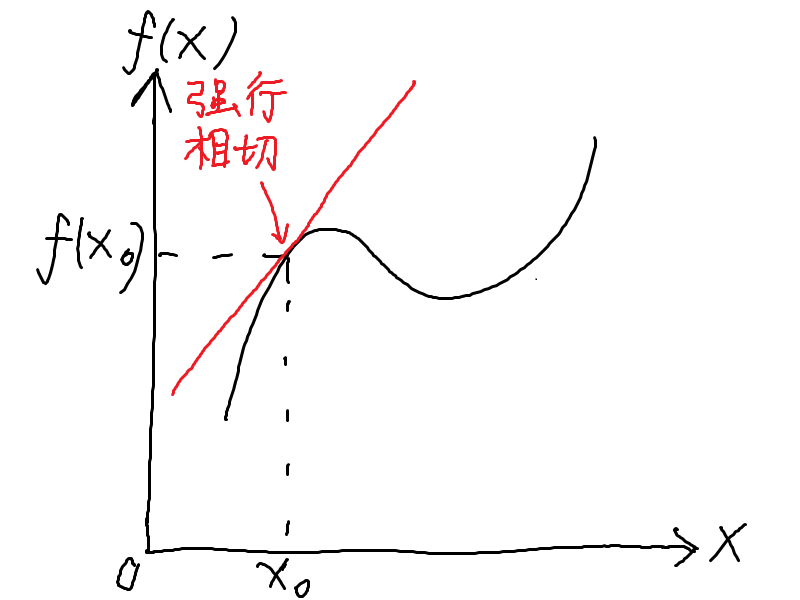
\includegraphics[scale=0.5]{fig/tangent.png}
\caption{一张灵魂插图}
\label{fig-tangent}
\end{figure}

但是怎么确定这条直线的斜率呢?如果真的只有$x_0$这一个点的话,这条直线是不能确定的,因为两个点才能确定一条直线。但是可以在它旁边再取一个点,然后画一条直线,如图\ref{fig-secant}。
\begin{figure}[htb]
\centering
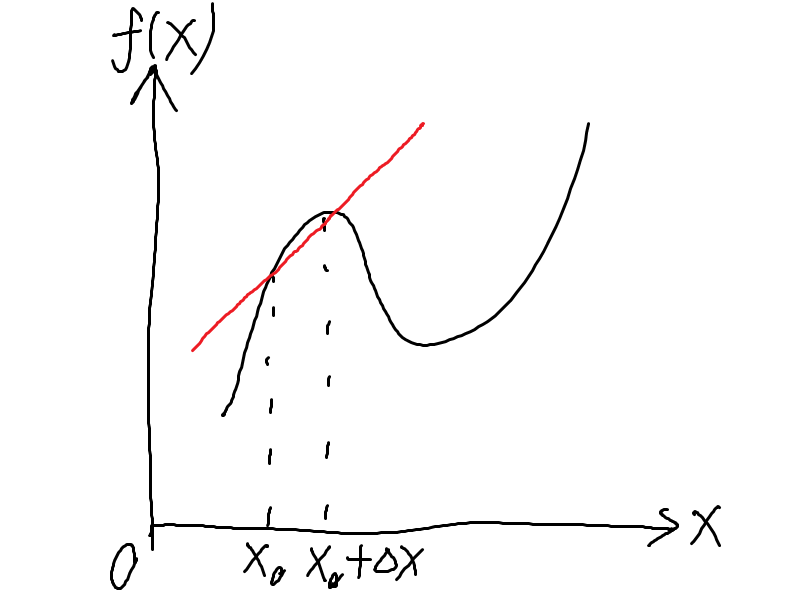
\includegraphics[scale=0.5]{fig/secant.png}
\caption{每张图下面都有标题是一个好习惯}
\label{fig-secant}
\end{figure}

这条直线的斜率就是$\frac{\Delta f}{\Delta x}=\frac{f(x_0+\Delta x)-f(x_0)}{\Delta x}$。$\Delta x$是一个无穷小的东西,但是它又不是$0$,因为它要出现在分母上。至于无穷小到底是什么意思,有兴趣的同学可以去看高数书上关于极限的内容。

举个栗子:如果$f(x)=x^2$,那么
\begin{align*}
&\mathrel{\phantom{=}}\frac{f(x_0+\Delta x)-f(x_0)}{\Delta x} \\
&=\frac{(x_0+\Delta x)^2-x_0^2}{\Delta x} \\
&=\frac{x_0^2+2 x_0 \Delta x+\Delta x^2-x_0^2}{\Delta x} \\
&=\frac{2 x_0 \Delta x+\Delta x^2}{\Delta x}
\end{align*}

上面这些都是初中就会的东西。然而这时候牛顿干了一件脑洞大开的事情,他说:既然$\Delta x$是一个无穷小的东西,那么$\Delta x^2$肯定比$\Delta x$还小,我们可以不管它。于是上面的式子变成了
\begin{align*}
&\mathrel{\phantom{=}}\frac{2 x_0 \Delta x+\Delta x^2}{\Delta x} \\
&=\frac{2 x_0 \Delta x}{\Delta x} \\
&=2 x_0
\end{align*}

也就是说$\ddx x^2=2 x$。这里$\ddx$表示对$x$求导,然而高中数学课本上把它写成$f'(x)$。

这里有几个名称上的问题需要注意:求导是一个把函数$f(x)$变成另一个函数$f'(x)$的操作,$f(x)$叫作原函数,$f'(x)$叫作导函数,简称导数。$x=x_0$时,$f(x)$的函数值为$f(x_0)$,导数为$f'(x_0)$,也可以写成$\ddx f(x)|_{x=x_0}$,比如$\ddx x^2|_{x=3}=6$。
\section{幂函数的导数}
再试一下$f(x)=x^3$的导数:
\begin{align*}
&\mathrel{\phantom{=}}\frac{(x_0+\Delta x)^3-x_0^3}{\Delta x} \\
&=\frac{x_0^3+3 x_0^2 \Delta x+3 x_0 \Delta x^2+\Delta x^3-x_0^3}{\Delta x} \\
&=\frac{3 x_0^2 \Delta x+3 x_0 \Delta x^2+\Delta x^3}{\Delta x} \\
&=\frac{3 x_0^2 \Delta x}{\Delta x} \\
&=3 x_0^2
\end{align*}

也就是说$\ddx x^3=3 x^2$。

再举一个平凡的例子:如果$f(x)=1$,那么$f(x)$的图像就是一条横线,显然$f'(x)=0$。(平凡的例子有时候很好用)

现在可以猜:对任何正整数$n$,$\ddx x^n=n x^{n-1}$。事实上对任何实数$n$(包括负数、分数甚至无理数),这句话都是对的,前提是$x^n$有定义,当然$-1^{\frac{1}{2}}$之类的东西在实数范围里是没有定义的。目前这句话是猜出来的,稍微严格一些的证明待会再讲。

但是!有一个特殊情况需要注意。$n=0$时,按照上式,$\ddx x^0=0 \cdot x^{-1}=0$。这么说有一定道理,但是严格来说$f'(x)=0$和$f'(x)=0 \cdot x^{-1}$ 的定义域是不一样的。

那么什么东西的导数是$1 \cdot x^{-1}$呢?高中课本告诉我们是$\ln x$,但是这件事情也要待会再讲。

【练习】求证$\ddx x^{-1}=-1 \cdot x^{-2}$,如果能算出来那么之前的东西应该都懂了。
\section{导数与加、减、乘法}
$\ddx(f+g)=\frac{\opd f}{\opd x}+\frac{\opd g}{\opd x}$,这应该很符合直觉。

既然我们知道负数,那么减法就是加法!减法就是加法!!减法就是加法!!!

在上式中令$f=g$,则$\ddx(2f)=\ddx(f+f)=2\frac{\opd f}{\opd x}$。仍然可以猜:$\ddx(c f)=c \frac{\opd f}{\opd x}$,$c$是任何实数。

(再次强调,把正整数改成实数就是为了包含负数、分数和无理数,而$0$经常成为一个特殊情况)(诶我这算是把实数理论讲完了吗)

这两个公式说明,求导这个操作是一个\emph{线性算符}。

(所谓算符就是一种操作,它把一个函数变成另外一个函数,有些地方翻译成算子。线性算符就是满足$L(a f+b g)=a L(f)+b L(g)$的算符,其中$a,b$是实数,$f,g$是函数)

举个栗子,$\ddx(2x^3+3x^2+4x+5)=6x^2+6x+4$,熟练之后这种多项式求导就可以口算了。

两个函数乘起来之后求导就会麻烦一些。可以想象一个长方形,它的一边长是$f(x)$,另一边长是$g(x)$,面积$S(x)=f(x) \cdot g(x)$。现在把两边分别增加$\Delta f$和$\Delta g$,如图\ref{fig-rect}。
\begin{figure}[htb]
\centering
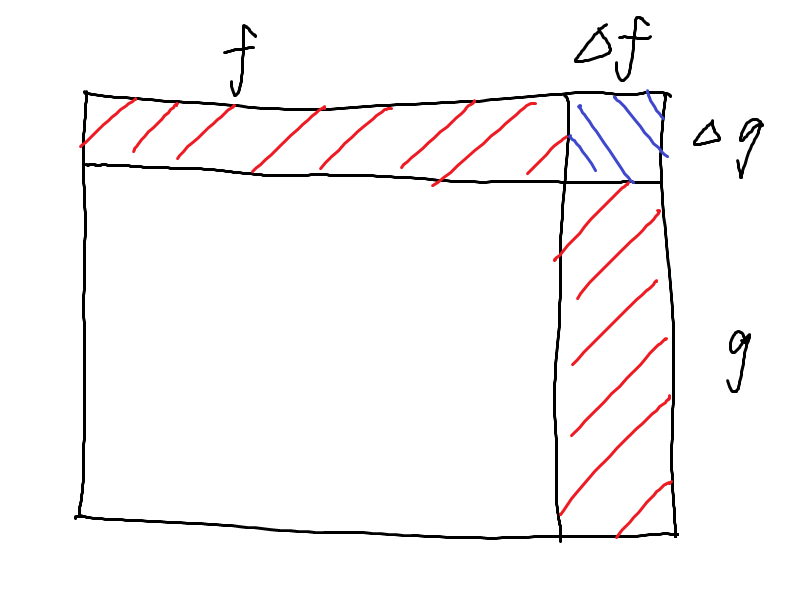
\includegraphics[scale=0.5]{fig/rect.png}
\caption{长方形的面积改变了多少呢?}
\label{fig-rect}
\end{figure}

$\Delta S=\Delta f \cdot g+f \cdot \Delta g+\Delta f \cdot \Delta g$,然而$\Delta f \cdot \Delta g$比$\Delta f \cdot g$和$f \cdot \Delta g$更小,所以就不管它了。

也就是说,$\ddx(f \cdot g)=\frac{\opd f}{\opd x} \cdot g+f \cdot \frac{\opd g}{\opd x}$。为了\emph{装逼},有些地方把这个公式叫作\emph{莱布尼兹律}。如果$g(x)$是常数$c$,这个公式就是上面乘$c$的公式。

同样我们知道,除法就是乘法!除法就是乘法!!除法就是乘法!!!但是两个函数相除的导数要待会再讲。
\section{$\rme^x$与它的导数;$\rme$到底是什么东西}
有没有一个函数的导数是它自己呢?常函数$f(x)=0$显然是这样的函数。幂函数不是这样的函数,因为求导之后幂指数要$-1$。但是把无穷多个幂函数加起来,就可以构造出这样的函数。

【练习】你可以自己先想一想怎么构造,跟无穷等比数列求和的方法差不多。

比如这个函数:($\exp$是函数的名字,表示exponent,跟$\sin$一样)
\begin{equation*}
\exp x=\sum_{n=0}^{\infty}\frac{x^n}{n!}
\end{equation*}

首先,看到求和号,不要怕,不要怕,不要怕。

这是无穷多个幂函数求和,但是结果并不是无穷大,而是一个有限的数。可以简单判断一下:每一项的分子是$x^n$,分母是$n!$,当$n$很大时,$n! \gg x^n$,每一项都趋于$0$,求和之后确实是一个有限的数。

(“$n$很大”指的是$n \gg x$,大家遇到“很大”“很小”的时候要想清楚谁远大于谁。)

如果把它一项一项写出来就是$1+x+\frac{1}{2}x^2+\frac{1}{6}x^3+\dots$,然后求导,可以发现导数真的跟原函数一样。

但是有一个问题:如果原函数$\times 2$,那么导数也会$\times 2$。如果一个函数满足“导数是它自己”这个要求,那么$\times 2$之后的函数也满足。上面这个$\exp x$的方便之处就在于$\exp 0=1$,所以大家都喜欢用它。可以证明,满足导数是它自己且$f(0)=1$这两个要求的函数有且只有这一个。(这是微分方程的事情,更严格的证明要等到函数空间)

$\exp 1$是一个数学中经常会遇到的数,我们把它叫作$\rme$,这就是高中课本中的$\rme \approx 2.718 \dots$。

有兴趣的同学可以用二项式的一些性质证明$\exp x \cdot \exp y=\exp(x+y)$。以后还可以证明,对任何实数$c$,$(\exp x)^c=\exp(c x)$。这就是指数函数满足的两条性质,所以对任何实数$x$,$\exp x=\rme^x$,它就是大家都知道的以$\rme$为底的指数函数。

有些地方会用另一个极限来定义$\rme$,而这里的定义是从“导数是它自己”这个要求出发的,看起来比较有道理。
\section{多元函数求导;复合函数求导;导数与除法;指数函数的导数}
如果函数$f(x,y)$与自变量$x$和$y$有关(注意现在$x$与$y$无关,或者说我们故意不管$x$与$y$的关系),可以单独对$x$或者$y$求导,只要把其他自变量当作常数就行了。比如$\ddx x^2 y^3=2 x y^3$,而$\ddy x^2 y^3=3 x^2 y^2$。

$\ddx f(x,y)$有时候会写成$\ppx f(x,y)$,来强调这是对多元函数求导。$\partial$称为偏微分算符,其实它和微分算符$\opd$没有什么区别。

($\partial$读作partial,但是很多中国人也会读作偏)

如果对$f(g(x))$这样的复合函数求导,可以把$\frac{\opd f}{\opd x}$拆开来变成$\frac{\opd f}{\opd g} \cdot \frac{\opd g}{\opd x}$。比如:

(诶为什么$f$一会在$\ddx$上面一会在$\ddx$右边呢?这只是书写的习惯问题,意思是一样的)
\begin{align*}
&\mathrel{\phantom{=}}\ddx \ln \frac{1}{x} \\
&=\frac{\opd \ln \frac{1}{x}}{\opd \frac{1}{x}} \cdot \frac{\opd \frac{1}{x}}{\opd x}
\internote{(把$\ln \frac{1}{x}$对“$\frac{1}{x}$”求导,而不是对$x$求导)}
&=\frac{1}{\frac{1}{x}} \cdot -\frac{1}{x^2} \\
&=-\frac{1}{x}
\end{align*}

刚才说过,除法就是乘法。先推导$\ddx \frac{1}{g(x)}=\frac{\opd \frac{1}{g(x)}}{\opd g(x)} \cdot \frac{\opd g(x)}{\opd x}=-\frac{\ddx g(x)}{g^2(x)}$,然后就能得到导数的除法公式$\ddx \frac{f(x)}{g(x)}=\ddx (f(x) \cdot \frac{1}{g(x)})=\frac{\frac{\opd f}{\opd x} \cdot g-f \cdot \frac{\opd g}{\opd x}}{g^2(x)}$。(注意哪个正哪个负!)

按照复合函数求导公式,与$x$相乘的系数在求导的时候可以提到前面,比如$\ddx \rme^{k x}=\frac{\opd \rme^{k x}}{\opd k x} \cdot \frac{\opd k x}{\opd x}=k \rme^{k x}$。

如果是一般的指数函数,$\ddx a^x=\ddx (\rme^{\ln a})^x=\ddx \rme^{\ln a \cdot x}=\ln a \cdot a^x$。
\section{反函数求导;对数函数的导数;填上幂函数的坑}
如果知道$y=f(x)$以及它的导数$\frac{\opd y}{\opd x}=\ddx f(x)$,而$x$可以用反函数$x=g(y)$表示出来,那么$\frac{\opd x}{\opd y}$可以直接用$\frac{1}{\frac{\opd y}{\opd x}}$表示出来。(我不喜欢$f^{-1}(y)$这种写法,会与$f^2(y)$的意思搞混)

比如$y=\exp x$,$x=\ln y$,我们已经知道$\frac{\opd y}{\opd x}=exp x$,那么
\begin{align*}
\frac{\opd x}{\opd y}&=\frac{1}{\frac{\opd y}{\opd x}} \\
&=\frac{1}{\exp x} \\
&=\frac{1}{y}
\end{align*}

也就是说$\ddy \ln y=\frac{1}{y}$。

如果是一般的对数函数,$\ddx \log_a x=\ddx \frac{\ln x}{\ln a}=\frac{1}{\ln a} \cdot \frac{1}{x}=\frac{1}{x \ln a}$。

刚才猜出来,对任何实数$n$,$\ddx x^n=n x^{n-1}$。现在证明:$\ddx x^n=\ddx (\rme^{\ln x})^n=\ddx \rme^{n \ln x}=n \rme^{n \ln x} \cdot \frac{1}{x}=n x^{n-1}$。

\section{三角函数、反三角函数的导数}

首先高中物理课本有这样一句话:$x$(弧度)很小的时候,$\sin x=x$。

(高中里定义三角函数用的是几何方法:如果直角三角形斜边长为$1$,一个角为$x$,那么对边为$\sin x$。和差化积之类的公式也是用几何方法证明的,所以现在看起来不够严谨。刚才用级数定义了指数函数,以后还可以用$\exp \rmi x=\cos x+\rmi \sin x$来定义三角函数。)

我们来看$\sin x$的导数:
\begin{align*}
&\mathrel{\phantom{=}}\sin(x_0+\Delta x)-\sin x_0 \\
&=2 \cos \frac{2x_0+\Delta x}{2} \sin \frac{\Delta x}{2} \\
&=2 \cos \frac{2x_0}{2} \cdot \frac{\Delta x}{2} \\
&=\cos x_0 \cdot \Delta x
\end{align*}

所以$\ddx \sin x=\cos x$。

【练习】证明$\ddx \cos x=-\sin x$,$\ddx \tan x=\frac{1}{\cos^2 x}$(用导数的除法公式)。

三角函数有很方便的性质:$\frac{\mathrm{d^2}}{\opd x^2}\sin x=-\sin x$,$\frac{\mathrm{d^2}}{\opd x^2}\cos x=-\cos x$。($\frac{\mathrm{d^2}}{\opd x^2}$表示对$x$求两次导)

设$y=\sin x$,$x=\arcsin y$,然后来看$\arcsin y$的导数:
\begin{align*}
\frac{\opd x}{\opd y}&=\frac{1}{\frac{\opd y}{\opd x}} \\
&=\frac{1}{\cos x} \\
&=\frac{1}{\sqrt{1-y^2}}
\end{align*}

所以$\ddx \arcsin y=\frac{1}{\sqrt{1-y^2}}$。

【练习】证明$\ddx \arccos x=-\frac{1}{\sqrt{1-x^2}}$,$\ddx \arctan x=\frac{1}{1+x^2}$(需要一些三角变形)。
\section{对方程求导;曲线的切线}
如果把方程的两边对同一个自变量求导,方程仍然成立。

举个栗子:求$x^x$的导数。诶这个东西不是幂函数也不是指数函数,怎么办?可以解方程:
\begin{align*}
y&=x^x
\internote{(既然有指数,可以两边取对数试试看)}
\ln y&=x \ln x \\
\frac{1}{y} \cdot \frac{\opd y}{\opd x}&=\ln x+1
\internote{(注意两边都是对$x$求导,如果左边对$y$求导右边对$x$求导就错了)}
\frac{\opd y}{\opd x}&=y(\ln x+1) \\
&=x^x (\ln x+1)
\end{align*}

这个方法可以求平面内任意曲线(不一定是函数图像)的切线。比如有一个椭圆$\frac{x^2}{a^2}+\frac{y^2}{b^2}=1$,上面有一个点$(x_0,y_0)$,容易算出$y_0=\pm b \cdot \sqrt{1-\frac{x^2}{a^2}}$。可以用黑科技求出过这个点的切线斜率,而不用设直线算$\Delta$之类的:

\begin{align*}
\frac{x^2}{a^2}+\frac{y^2}{b^2}&=1 \\
\frac{2x}{a^2}+\frac{2y}{b^2} \cdot \frac{\opd y}{\opd x}&=0
\internote{(注意$y$与$x$有关,而$a$和$b$是常数)}
\frac{\opd y}{\opd x}&=-\frac{b^2 x}{a^2 y} \\
&=\pm \frac{b x_0}{a \sqrt{a^2-x_0^2}}
\end{align*}

这个斜率前面有$\pm$,因为现在把它表示成$x_0$的函数,而一个$x_0$对应椭圆上的两个点,所以有两条切线,到底是哪一条要看情况判断。
\section{什么样的函数是可以求导的}
到这里为止我们已经可以动手算很多导数了,但是有的函数在某些点根本就不能求导,这种情况在高中是大家都不关心的,但是我们要留个心眼。

常见的人畜无害的函数有幂函数、指数函数、对数函数、三角函数、反三角函数,以及它们经过有限次加、乘、复合构成的函数,它们叫作\emph{初等函数}。初等函数在它们的定义域内都是可以求导的。(无限次复合就会出现奇怪的事情,现在不去管它)

一个函数要求导,首先要求它的图像是连续的,在断掉(比如某些高中数学老师拍脑袋想出来恶心别人的分段函数)的点是不行的,爆掉(趋于$+\infty$或$-\infty$,英文就是blow up)的点也是不行的,如图\ref{fig-bad-deri}。
\begin{figure}[htb]
\centering
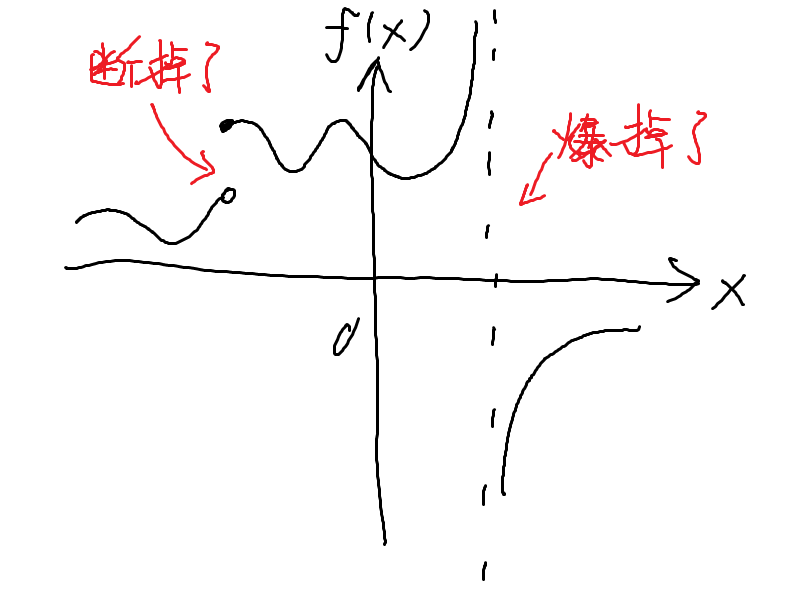
\includegraphics[scale=0.5]{fig/bad-deri.png}
\caption{画图记得原点和坐标轴的名字}
\label{fig-bad-deri}
\end{figure}

如果分段函数的图像没有断掉,可以算一下两边的导数,如果不同,那么在分割点就不能求导;如果相同,那么分割点的导数就是它了。

比如绝对值函数$f(x)=|x|$,左边的导数是$-1$,右边的导数是$+1$,两边不同,那么$x=0$时就不能求导。而两边导数相同的函数比如(灵魂画师表示懒得画图了,大家自己画吧)
\begin{equation*}
f(x)=
\begin{cases}
2x, &x \le 1 \\
x^2+1, &x>1
\end{cases}
\end{equation*}

那么$\ddx f(x)|_{x=1}=2$。

狄利克雷曾经构造出了处处不连续的函数,而魏尔斯特拉斯构造出了更加丧心病狂的处处连续但不可导的函数。
\section{积分就是导数的逆运算}
把这节的标题读一遍,然后就讲完了。各种奇怪的换元等到要用的时候再讲。如果你对微积分还不熟悉,要注意不定积分和定积分的关系、积分常数,还可以去高数书上看看分部积分法。

悲剧的是,不是所有初等函数的积分都可以算出来(用初等函数表示),比如$\rme^{-x^2}$、$\frac{\sin x}{x}$的积分都是算不出来的。

【练习】自己写一遍幂函数、指数函数、对数函数、三角函数、反三角函数的导数和积分表。
\section{睡前小故事:$\sqrt{-1}$与$\frac{1}{0}$}
在实数范围内,$\sqrt{-1}$是不存在的。然而我们硬要定义$\rmi=\sqrt{-1}$(的一个值),于是就有了复数。那么能不能定义一个$\rmj=\frac{1}{0}$呢?硬要定义的话确实可以,但是这样一来世界上就只剩下一个实数了,我们觉得这样做很不好。

诶这是什么情况?首先来整理一下,实数满足这样几条公理(这里列出的不全,但是够用了):
\begin{enumerate}
\item 存在一种运算叫加法,它把两个实数变成一个实数。(不要小看关于存在性的公理!迟早有一天我们会被存在性坑一发!)
\item $(a+b)+c=a+(b+c)$。(加法结合律)
\item $a+b=b+a$。(加法交换律,以后会发现很多时候结合律比交换律更重要)
\item 存在一个实数叫$0$,使得对任何实数$a$,$a+0=a$。
\item 存在一种运算叫减法,它是加法的逆运算,也就是说对任何实数$a$,$a-a=0$。
\item 存在一种运算叫乘法,它把两个实数变成一个实数。
\item $(a \cdot b) \cdot c=a \cdot (b \cdot c)$。(乘法结合律)
\item $a \cdot b=b \cdot a$。(乘法交换律)
\item 存在一个实数叫$1$,使得对任何实数$a$,$a \cdot 1=a$。
\item 存在一种运算叫除法,它是乘法的逆运算,也就是说对任何不为$0$的实数$a$,$\frac{a}{a}=1$。(“不为$0$”意味着$0$和$1$的地位不一样,加法和乘法的地位也不一样)
\item 乘法分配律。(这是加法和乘法另一个不一样的地方)
\end{enumerate}

而等号满足这样几条公理:
\begin{enumerate}
\item $a=a$。
\item 如果$a=b$,那么$b=a$。
\item 如果$a=b$,$b=c$,那么$a=c$。
\end{enumerate}

诶你怎么还没睡着?所谓公理就是这些看起来像废话的东西,但是所有的证明必须严格按照它们来推导。比如证明任何一个实数乘$0$等于$0$:
\begin{align*}
a \cdot b&=a \cdot b \\
a \cdot (b+0)&=a \cdot b \\
a \cdot b+a \cdot 0&=a \cdot b \\
a \cdot 0&=0
\end{align*}

这件事情符合我们的直觉,而公理也保证了这件事情的严谨性。如果定义一个$\rmi$,这几条公理仍然是满足的,所以大家觉得这件事情很好。

但是!如果定义一个$\rmj$,这几条公理就会出问题,因为它在直接挑战$0$和$1$的地位。

既然定义了$\rmj$,那么除法的定义里的“不为$0$”应该去掉。然后按上面的公理来推导:
\begin{align*}
0 \cdot \rmj&=1 \\
a \cdot (0 \cdot \rmj)&=a \cdot 1 \\
(a \cdot 0) \cdot \rmj&=a \cdot 1 \\
0 \cdot \rmj&=a
\end{align*}

同理可得$0 \cdot \rmj=b$,所以$a=b$。也就是说,世界上只剩下一个实数了。如果硬要让$a \neq b$,那么乘法结合律、乘法分配律或者等号满足的公理就会出问题,那就更不好了。

\chapter{复变函数与级数}
\rightline{\it 学习复变函数之前要大喊三声:变变变!}
\section{用级数定义一些函数}
什么是复数应该不用我说了。但是你能说清楚$2$的$\rmi$次方是什么意思吗?如果说$\rmi$个$2$相乘就很难理解。现在重新定义一下以前学过的函数,让它们在复数范围内也能用,这些工作叫作\emph{解析延拓}。

前面用级数定义了$\exp x=\sum_{n=0}^{\infty}\frac{1}{n!}x^n=1+x+\frac{1}{2}x^2+\frac{1}{6}x^3+\dots$。不管$x$是实数还是复数,这样的定义都能用。

借助欧拉公式$\exp \rmi x=\cos x+\rmi \sin x$就能定义$\sin x$和$\cos x$。把$\exp \rmi x$打开得到$1+\rmi x-\frac{1}{2}x^2-\frac{1}{6} \rmi x^3+\frac{1}{24} x^4+\frac{1}{120} \rmi x^5-\dots$,然后把实部和虚部分开,得到
\begin{align*}
\sin x&=\sum_{n=0}^{\infty}\frac{1}{(2n+1)!}x^{2n+1}=x-\frac{1}{6}x^3+\frac{1}{120}x^5+\dots \\
\cos x&=\sum_{n=0}^{\infty}\frac{1}{(2n)!}x^{2n}=1-\frac{1}{2}x^2+\frac{1}{24}x^4+\dots
\end{align*}

可以看出$\sin x$是奇函数,$\cos x$是偶函数。为了产生波浪的形状,它们的各项系数是一正一负的。直接求导会发现$\ddx \sin x=\cos x$,$\ddx \cos x=-\sin x$。有兴趣的同学经过一通暴算还会发现$\sin^2 x+\cos^2 x=1$。

但是用级数定义三角函数也有不方便的地方,比如一眼看不出来$\sin \pi=0$(这件事情的证明要等到傅立叶级数),所以有时候我们也会用到几何定义。如果$x$是复数,$\sin x$和$\cos x$的几何意义比较难理解,现在我们只要知道它们是级数就行了。

然后可以定义$\ln x$:如果$\exp x=y$,那么$\ln y=x$。但是奇怪的事情出现了:我们已经知道$\exp 2 \pi \rmi=1$,那么$\ln \exp 2 \pi \rmi=\ln 1$,$2 \pi \rmi=0$?

事实上,不同的$x$可以有相同的$\exp x$,所以$\exp x$的反函数不是单值的,跟反三角函数会出现的问题一样。多值函数的事情以后再讲,现在可以定义:如果$\opIm x \in [0,2\pi)$ 且$\exp x=y$,那么$\ln y=x$。($\opIm x$表示$x$的虚部)

现在任何非零复数的对数都有定义,然后可以定义一般的幂运算:$(a+b \rmi)^{c+d \rmi}=(\rme^{\ln(a+b \rmi)})^{c+d \rmi}=\exp((c+d \rmi)\ln(a+b \rmi))$(要求$a+b \rmi \neq 0$)。这样一来,任何非零复数的复数次方都有了定义,然而零仍然是一个麻烦的问题。

还要注意一下,前面讲的求导和积分都是在一维的情况下的,现在自变量可以在二维的复平面上移动,求导和积分的几何意义都有一些变化,但是之前的公式仍然可以套上去。
\section{三角函数的指数形式;双曲函数}
$\sin x$和$\cos x$可以用$\exp x$表示出来:
\begin{align*}
\sin x&=\frac{1}{2 \rmi}(\rme^{\rmi x}-\rme^{-\rmi x}) & \cos x&=\frac{1}{2}(\rme^{\rmi x}+\rme^{-\rmi x})
\end{align*}

虽然公式中出现了复数,但最后的结果一定是实数。如果把$\rmi$去掉,可以定义:
\begin{align*}
\sinh x&=\frac{1}{2}(\rme^x-\rme^{-x}) & \cosh x&=\frac{1}{2}(\rme^x+\rme^{-x})
\end{align*}

它们叫作双曲正弦和双曲余弦函数,多出来的h表示双曲(hyperbolic)。这就是传说中高中老师不讲,大学老师以为讲过的东西。容易证明以下的关系:(你应该可以口算)
\begin{align*}
\sinh x&=-\rmi \sin \rmi x & \cosh x&=\cos \rmi x \\
\sin x&=-\rmi \sinh \rmi x & \cos x&=\cosh \rmi x \\
\ddx \sinh x&=\cosh x & \ddx \cosh x&=\sinh x \\
& & \cosh^2 x-\sinh^2 x&=1
\end{align*}

还可以定义双曲正切函数$\tanh x=\frac{\sinh x}{\cosh x}=\frac{\rme^x-\rme^{-x}}{\rme^x+\rme^{-x}}$,可以写成$\frac{1}{2}\tanh\frac{x}{2}=\frac{1}{2}-\frac{1}{\rme^x+1}$。这是一个奇函数,高考数学里好像经常出现这个,以后讲统计力学的时候还会遇到它。
\section{关于三角函数的一些黑科技}
把三角函数表示成指数可以方便地推导积化和差公式:
\begin{align*}
&\pheq\cos a \cos b \\
&=\frac{1}{4}(\rme^{\rmi a}+\rme^{-\rmi a})(\rme^{\rmi b}+\rme^{-\rmi b}) \\
&=\frac{1}{4}(\rme^{\rmi (a+b)}+\rme^{\rmi (-a+b)}+\rme^{\rmi (a-b)}+\rme^{\rmi (-a-b)}) \\
&=\frac{1}{2}(\cos(a+b)+\cos(a-b))
\end{align*}

【练习】证明$\sin a \sin b=\frac{1}{2}(-\cos(a+b)+\cos(a-b))$。

还可以用来计算一些积分:
\begin{align*}
&\pheq\int \rme^{a x} \sin b x \opd x \\
&=\frac{1}{2 \rmi}\int \rme^{a x}(\rme^{\rmi b x}+\rme^{-\rmi b x})\opd x \\
&=\frac{1}{2 \rmi}\int (\rme^{(a+\rmi b)x}+\rme^{(a-\rmi b)x})\opd x \\
&=\frac{1}{2 \rmi}(\frac{\rme^{(a+\rmi b)x}}{(a+\rmi b)}+\frac{\rme^{(a-\rmi b)x}}{(a-\rmi b)})+C
\internote{(经过一坨暴算)}
&=\frac{\rme^{a x}(a \sin b x-b \cos b x)}{a^2+b^2}+C
\end{align*}

【练习】证明$\int \rme^{a x} \cos b x \opd x=\frac{\rme^{a x}(a \cos b x+b \sin b x)}{a^2+b^2}+C$。

$\phantom{\text{【练习】}}$证明$\int \cos a x \cos b x \opd x=\frac{\sin(a+b) x}{2 (a+b)}+\frac{\sin(a-b) x}{2 (a-b)}+C$,想一想需要讨论的特殊情况,以及它们的几何或者物理意义。

如果要对三角函数求和,可以先对指数函数求和,再把指数函数表示成三角函数:
\begin{align*}
\sum_{k=1}^{n}\rme^{\rmi k x}&=\rme^{\rmi x}+\rme^{2 \rmi x}+\rme^{3 \rmi x}+\dots+\rme^{n \rmi x} \\
&=\frac{\rme^{\rmi x}-\rme^{(n+1) \rmi x}}{1-\rme^{\rmi x}} \\
&=\frac{\cos x+\rmi \sin x-\cos(n+1)x-\rmi \sin(n+1)x}{1-\cos x-\rmi \sin x}
\internote{(经过一坨暴算)}
&=\frac{\sin \frac{n x}{2} \cos \frac{(n+1) x}{2}}{\sin \frac{x}{2}}+\rmi \frac{\sin \frac{n x}{2} \sin \frac{(n+1) x}{2}}{\sin \frac{x}{2}}
\end{align*}

把实部和虚部分开,得到
\begin{align*}
\sum_{k=1}^{n}\cos k x&=\frac{\sin \frac{n x}{2} \cos \frac{(n+1) x}{2}}{\sin \frac{x}{2}} \\
\sum_{k=1}^{n}\sin k x&=\frac{\sin \frac{n x}{2} \sin \frac{(n+1) x}{2}}{\sin \frac{x}{2}}
\end{align*}
\section{反双曲函数与反三角函数}
双曲函数的定义式可以化成关于$\rme^x$的二次方程,然后可以把它们的反函数解出来:
\begin{align*}
\arsinh x&=\ln(x+\sqrt{x^2+1}) & \arcosh x&=\pm \ln(x+\sqrt{x^2-1})
\end{align*}

这里的ar的意思不是弧(arc),而是面积(area)。$\sinh x$是奇函数,因此它的反函数也是奇函数,高考数学里好像也会出现这个。$\cosh x$是偶函数,因此它的反函数前面有$\pm$。

反三角函数可以表示成同样的形式(在合适的值域下):
\begin{align*}
\arcsin x&=-\rmi \ln(\rmi x+\sqrt{-x^2+1}) & \arccos x&=\pm \rmi \ln(\rmi x+\sqrt{-x^2-1})
\end{align*}

【练习】证明$\arcsin \frac{1}{2}=\frac{\pi}{6}$。
\section{泰勒级数}
前面把$\exp x$、$\sin x$和$\cos x$用(指数是正整数的)多项式表示了出来,但是$\ln x$不能用多项式表示出来,因为没有哪个多项式在$x=0$时爆掉。

在$x=1$附近$\ln x$ 就不会爆掉,而且可以求任意多次导,这样的性质跟多项式一样,因此可以用多项式近似地表示出$\ln(1+x)$。这里的“近似”指的是:找到这样一个多项式$T(x)=a_0+a_1 x+a_2 x^2+\dots$,使得它在$x=0$处的值和任意阶导数都与$\ln(1+x)$相等。
\begin{align*}
& & \ln(1+x)|_{x=0}&=0 \\
\ddx \ln(1+x)&=\frac{1}{1+x} & \ddx \ln(1+x)|_{x=0}&=1 \\
\ddxn{2} \ln(1+x)&=-\frac{1}{(1+x)^2} & \ddxn{2} \ln(1+x)|_{x=0}&=-1 \\
\ddxn{3} \ln(1+x)&=\frac{2}{(1+x)^3} & \ddxn{3} \ln(1+x)|_{x=0}&=2 \\
&\dots \\
\ddxn{n} \ln(1+x)&=(-1)^{n-1} \frac{(n-1)!}{(1+x)^n} & \ddxn{n} \ln(1+x)|_{x=0}&=(-1)^{n-1} (n-1)!
\end{align*}

(看起来计算量很大是不是?就是这样)

如果$T(x)=\sum_{n=1}^{\infty} (-1)^{n+1} \frac{1}{n} x^n=x-\frac{1}{2}x^2+\frac{1}{3}x^3-\dots$,对它求导就会发现它满足“$x=0$处的值和任意阶导数都与$\ln(1+x)$相等”这个条件。这样的多项式叫作泰勒级数。

函数$f(x)$的泰勒级数可以表示为$\sum_{n=1}^{\infty} \frac{1}{n!} f^{(n)}(0) x^n$,其中$f^{(n)}(x)$表示$f(x)$的$n$阶导数。当然泰勒级数存在的前提是这些导数都存在(也就是说$f(x)$是\emph{光滑}的)。

$\ln x$的增长速度比任何多项式都慢,所以各项系数是一正一负的。而$\exp x$的增长速度比任何多项式都快,所以各项系数都是正的。

但是!$\ln x$的泰勒级数的收敛性没有那么容易证明。$x=-1$时,$T(x)=1+\frac{1}{2}x^2+\frac{1}{3}x^3+\dots$,你应该听说过这个级数是发散的。而$x=-1$时,$\ln(1+x)$确实爆掉了。

对于初等函数,泰勒级数的收敛性可以这样判断:在复平面上画出所有爆掉的点,找到离原点最近的点,以它到原点的距离为半径画一个圆,在圆内泰勒级数一定收敛,并且等于原来的函数,在圆外一定发散,在圆上则不一定。

泰勒级数把任何函数表示成多项式,这样会对一些计算带来方便。除了泰勒级数,还有很多有用的级数,比如洛朗级数、傅立叶级数、勒让德级数等等,它们把原来的函数表示成不同的形式,以后会慢慢讲。

【练习】求$\frac{1}{1+x}$和$\frac{1}{(1+x)^2}$的泰勒级数。
\section{小量近似}
如果不关心泰勒级数前面的系数,可以直接写成$f(x)=\sum_{n=1}^{\infty} a_n x^n=a_0+a_1 x+a_2 x^2+\dots$。$|x| \ll 1$时,可以把$x^2$以及更高阶的项都忽略,只剩下$a_0+a_1 x$,或者写成$a_0(1+k x)$。所以我们经常用到$\sin x=x$,$\cos x=1- \frac{1}{2}x^2$等等。

研究物理问题时经常从最低阶近似开始研究,它往往就是问题中最重要的东西,“真空中的球形鸡”就是这么来的。但是一阶项为$0$时,就要研究二阶项,甚至更高阶的项。比如$\cos x$是偶函数,它的一阶项为$0$,而二阶项是$-\frac{1}{2} x^2$。

小量运算中最重要的公式就是$(1+x)^n=1+n x$。举个栗子:
\begin{align*}
\tanh x&=\frac{\rme^x-\rme^{-x}}{\rme^x+\rme^{-x}} \\
&=\frac{(1+x)-(1-x)}{(1+x)+(1-x)} \\
&=x
\end{align*}

所以$x$很小时$\tanh x=x$。还可以发现$x$很大时$\tanh x=1$。如果你做实验发现一个$y$在$x$很小时与$x$成正比,而$x$很大时趋于不变,那么$\tanh x$可以在中间作为一个平滑的过渡,这种方法称为内插法。当年普朗克发现黑体辐射的公式,就是对适用于短波的维恩公式和适用于长波的瑞利-金斯公式进行了内插,并且发现这样做的物理意义是能量的量子化。内插法以后应该会专门讲。

$\arctan x$具有类似的性质,在$x$很小时等于$x$,$x$很大时等于$\frac{\pi}{2}$。

把$\tanh x$展开到更高阶会怎么样呢?它是奇函数,所以二阶项为$0$,现在来算三阶项:
\begin{align*}
\tanh x&=\frac{\rme^x-\rme^{-x}}{\rme^x+\rme^{-x}} \\
&=\frac{(1+x+\frac{1}{2} x^2+\frac{1}{6} x^3)-(1-x+\frac{1}{2} x^2-\frac{1}{6} x^3)}{(1+x+\frac{1}{2} x^2+\frac{1}{6} x^3)+(1-x+\frac{1}{2} x^2-\frac{1}{6} x^3)} \\
&=\frac{x+\frac{1}{6} x^3}{1+\frac{1}{2} x^2}
\end{align*}

现在要把分母翻上来,因为要算的是$x$的三阶项,所以所有中间过程必须保留到$x$的三阶项。可以先算出$(1+t)^{-1}=1-t$($t^2$超过$x$的三阶,不用算了),然后代入$t=\frac{1}{2} x^2$,得到$(1+\frac{1}{2} x^2)^{-1}=1-\frac{1}{2} x^2$。
\begin{align*}
\tanh x&=(x+\frac{1}{6} x^3)(1-\frac{1}{2} x^2) \\
&=x+\frac{1}{6} x^3-\frac{1}{2} x^3 \\
&=x-\frac{1}{3} x^3
\end{align*}

这样就得到了比$\tanh x=x$更准确一些的近似。
\section{复合函数的泰勒级数}
如果要计算$f(g(x))$在$0$附近的泰勒级数,先把$g(x)$在$0$附近的泰勒级数算出来,再代入$f(y)$在$g(0)$附近的泰勒级数就行了。

比如计算$\exp \sin x$的泰勒级数,保留到三阶。在$0$附近,$\sin x=x-\frac{1}{6} x^3$。而$\sin 0$刚好是$0$,在$0$附近,$\exp y=1+y+\frac{1}{2} y^2+\frac{1}{6} y^3$,所以
\begin{align*}
\exp \sin x&=1+(x-\frac{1}{6} x^3)+\frac{1}{2}(x-\frac{1}{6} x^3)^2+\frac{1}{6}(x-\frac{1}{6} x^3)^3 \\
&=1+(x-\frac{1}{6} x^3)+\frac{1}{2} x^2+\frac{1}{6} x^3
\intertext{(括号里的东西只要保留到三阶)}
&=1+x+\frac{1}{2} x^2
\end{align*}

三阶项刚好消掉了。有兴趣的同学如果继续算,会发现下一项到八阶的时候才不为0。

要注意的是,如果$g(0) \ne 0$,$f(y)$在$g(0)$附近的泰勒级数就没有这么容易计算。

【练习】求$\exp \ln(1+x)$的泰勒级数,保留到三阶。结果当然是$1+x$。
\section{算符级数;位移算符$\rme^{a \ddx}$}
把一个函数表示成级数之后,可以把它的自变量换成一些奇怪的东西,比如$\ddx$之类的算符。

比如$\rme^{a \ddx}$的级数展开是
\begin{equation*}
\rme^{a \ddx}=\sum_{n=0}^{\infty} \frac{1}{n!} a^n \ddxn{n}=1+a \ddx+\frac{1}{2} a^2 \ddxn{2}+\frac{1}{6} a^3 \ddxn{3}+\dots
\end{equation*}

你可能看不出来$\ddx$放在指数上是什么意思,但是在它的右边“乘”上一个函数$f(x)$,它就可以把$f(x)$变成另一个函数:
\begin{equation*}
\rme^{a \ddx} f(x)=\sum_{n=0}^{\infty} \frac{1}{n!} a^n \ddxn{n} f(x)=1+a \ddx f(x)+\frac{1}{2} a^2 \ddxn{2} f(x)+\frac{1}{6} a^3 \ddxn{3} f(x)+\dots
\end{equation*}

事实上,如果$f(x)$(在某个定义域内)是光滑的,那么$\rme^{a \ddx} f(x)=f(x+a)$。

$\rme^{a \ddx}$是一个线性算符,把$f(x)$展开成$a_0+a_1 x+a_2 x^2+\dots$,可以分开来算$\rme^{a \ddx}$对它们的作用。比如算$x^2$这一项:
\begin{align*}
\rme^{a \ddx} x^2&=1+a \ddx x^2+\frac{1}{2} a^2 \ddxn{2} x^2 \\
&=1+2 a x+a^2 \\
&=(x+a)^2
\end{align*}

利用二项式的公式可以证明,对所有正整数$n$,$\rme^{a \ddx} x^n=(x+a)^n$,合起来就是$\rme^{a \ddx} f(x)=f(x+a)$,相当于把$f(x)$的图像向左移动距离$a$,所以它称为位移算符。
\section{睡前小故事:$n$次多项式有$n$个根}
这件事情就是传说中的代数基本定理,现在我们要用一种炫酷的方法证明它。首先要知道,证明$n$次多项式有$n$个根,只要证明有一个根就行了,然后把这个根通过因式分解分出来,剩下$n-1$次多项式,重复这个过程就可以找到$n$个根。

设多项式为$f(z)=a_0 +a_1 z+a_2 z^2+\dots+a_n z^n$,$z$和$f(z)$都可以是复数,$f(z)=0$就是要让$\opRe f(z)=0$且$\opIm f(z)=0$。

当$|z|$很大时,忽略低阶项,$f(z)=a_n z^n$。设$z=r \rme^{\rmi \theta}$,那么$f(z)=a_n r^n \rme^{\rmi n \theta}$,$\opRe f(z)=0$就是要让$n \theta=(k+\frac{1}{2})\pi$,$\theta=(\frac{k}{n}+\frac{1}{2n})\pi$。

$\theta \in [0,2\pi)$,那么$\opRe f(z)=0$对应的就是$2n$条射线,同理$\opIm f(z)=0$对应的是另外$2n$条射线,$n=3$时如图\ref{fig-poly-root-outer}。
\begin{figure}[htb]
\centering
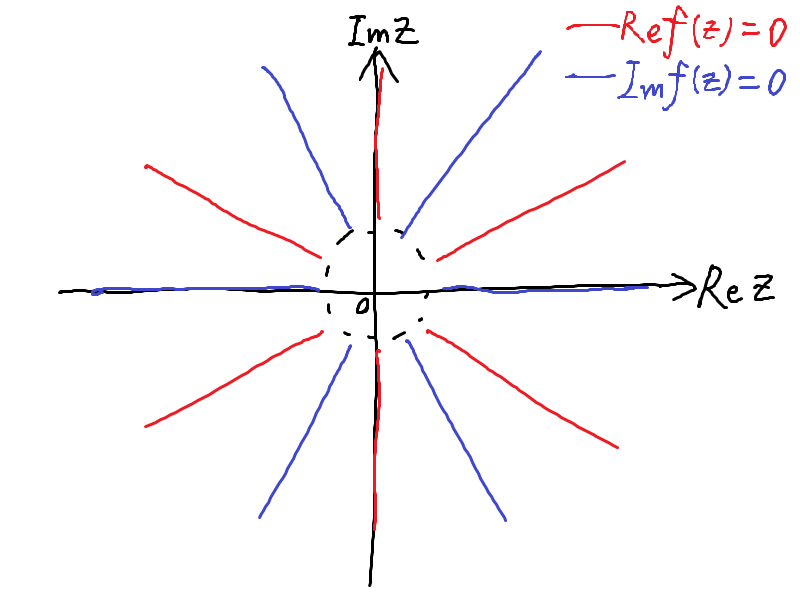
\includegraphics[width=0.33\linewidth]{fig/poly-root-outer.png}
\caption{$n=3$,$|z|$很大时$\opRe f(z)=0$和$\opIm f(z)=0$的图像}
\label{fig-poly-root-outer}
\end{figure}

其中红线为$\opRe f(z)=0$的图像,蓝线为$\opIm f(z)=0$的图像,黑圈里的情况现在还不知道,一种可能的情况如图\ref{fig-poly-root-inner},红线和蓝线的交点就是$f(z)=0$的根。
\begin{figure}[htb]
\centering
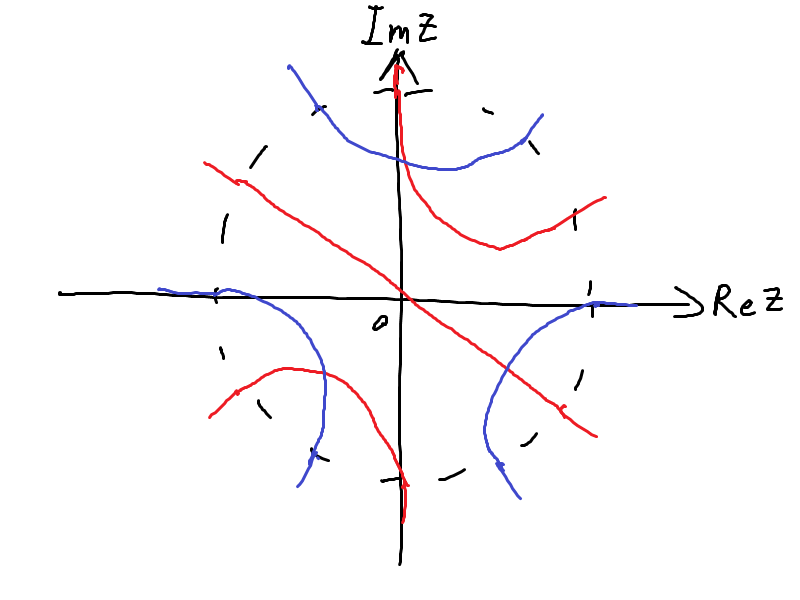
\includegraphics[width=0.33\linewidth]{fig/poly-root-inner.png}
\caption{$n=3$,$|z|$不太大时$\opRe f(z)=0$和$\opIm f(z)=0$可能的图像}
\label{fig-poly-root-inner}
\end{figure}

但是$f(z)$是一个光滑的函数,那么圈里的红线应该把圈外的红线两个一组相连,而且不会出现三条线交叉在同一点的情况,否则就不光滑了。如果四条线交叉在同一点,我们可以把交叉点分开,当作它们没有相交。蓝线也是这样。

于是“$n$次多项式有$n$个根”这个问题被我们转化为了一道炫酷的奥数题:圆周上相间排列着$2n$个红点和$2n$个蓝点,用不相交的红线把红点两个一组相连,不相交的蓝线把蓝点两个一组相连,求证红线和蓝线一定相交。用奇偶性很容易证明。

当然没有哪本高数书会讲这么炫酷的方法,我参考的是克莱因的《高观点下的初等数学》。

\chapter{微分方程}
\section{分离变量}
首先什么是微分方程呢?如果我们不知道一个函数$y(x)$的表达式,但是知道$\frac{\opd y}{\opd x}$与$x$、$y$的一些关系,然后就能把$y(x)$的表达式求出来,这样的方程就叫作微分方程。

举个栗子,一个地方的人口越多,人口增长得就越快。我们建立一个简单的模型,设人口为$y$,时间为$t$,那么$\frac{\opd y}{\opd t}=a y$,$a$是一个比例系数。可以这样解这个方程:
\begin{align*}
\frac{\opd y}{\opd t}&=a y \\
\frac{\opd y}{y}&=a \opd t
\internote{(现在$y$在方程的一边,$t$在方程的另一边,这种方法叫做\emph{分离变量})}
\ln y&=a t+C
\internote{(两边同时积分,本来都有积分常量,但是只要写一个$C$,另一个可以移到对面)}
y&=\exp(a t+C) \\
&=y_0 \exp a t
\end{align*}

其中$y_0=\exp C$,表示初始时的人口。如果初始时一个人都没有,以后当然不会有人出现。这就是高中生物课本上的J形增长曲线,所以生物学中很多图的纵坐标是数量的对数。

【练习】S形增长曲线满足$\frac{\opd y}{\opd t}=a y(K-y)$,先猜一猜这个方程是什么意思,然后把它解出来。

只有$\frac{\opd y}{\opd t}=a y$ 是无法确定$y_0$ 的,需要一个另外的条件才能确定,比如直接告诉你初始人口,也可以是一年后的人口。但是只要有一个条件,其他时候的人口就确定了,如果有更多的条件,就有可能自相矛盾(比如某些高中物理老师拍脑袋想出来的电磁感应题)。这种条件叫做\emph{边界条件}。(有些地方把边界条件叫作初始条件,我自己也分不清楚)

积分常量没有确定的时候,微分方程的解叫做\emph{通解},而积分常量确定之后,微分方程的解叫做\emph{特解}。上面这个方程中有$y$的一阶导数,所以叫做一阶微分方程。$n$阶微分方程需要$n$次积分才能解出来,通解有$n$个积分常量,需要$n$个边界条件才能确定特解。

话说有单位的东西叫作“量”,没有单位的东西叫作“数”,这件事情等到量纲分析再仔细讲。

悲剧的是,很多微分方程都是解不出来的(用初等函数表示)。就算能分离变量,接下来的积分也不一定能积出来。能用分离变量法解出来的都是一些最简单的微分方程,但是一般够用了,复杂的方法比如积分因子和花式换元法以后再讲。($\leftarrow$有生之年)
\section{线性常系数齐次微分方程;直接猜出解}
把待求函数设为$y(x)$,现在来看另一种简单的微分方程:
\begin{equation*}
a_0 y+a_1 y'+a_2 y''+\dots+a_n y^{(n)}=0
\end{equation*}

线性在数学的不同领域中有不同的意思,在这里是指方程中$y$和它的各阶导数最多只有一次项,而没有相乘的项,比如$y^2,y'^2,y \cdot y'$都不行。常系数指的是$y$和它的各阶导数不会和$x$相乘,也就是说$a_0,a_1,a_2\dots$都是常量。齐次指的是方程右边为零。这些名字现在记不住也没关系,以后会知道为什么这样的方程特别简单。

现在可以猜:$y=\rme^{\rmi k x}$。这样$y'=\rmi k \rme^{\rmi k x}=\rmi k y$,$y^{(n)}=(\rmi k)^n y$,这就是指数函数的好处。

代入方程得到$a_0 y+a_1 \rmi k y+a_2 (\rmi k)^2 y+\dots+a_n (\rmi k)^n y=0$,约掉$y$得到$a_0+a_1 \rmi k+a_2 (\rmi k)^2+\dots+a_n (\rmi k)^n=0$。这样就把关于$y$的微分方程转化为了关于$k$的代数方程。当然二次以上的代数方程我们还是不能手算,所以接下来只考虑二阶以下的微分方程。
\section{简谐振动;解的线性叠加}
把待求函数设为$x(t)$,然后来看这个方程:(有些地方用$\dot x$表示$\frac{\opd x}{\opd t}$,但是写到黑板上会看不清)
\begin{equation*}
x''+\omega_0^2 x=0
\end{equation*}

这就是简谐振动的微分方程。对于弹簧振子,$\omega_0^2=\frac{k}{m}$;对于单摆,$\omega_0^2=\frac{g}{l}$。

如果$x$是小球的位移,它应该是个实数,但是我们先允许它是复数,这样计算会方便一些。设$x=\rme^{\rmi \omega t}$,用刚才的方法得到$-\omega^2+\omega_0^2=0$,$\omega=\pm \omega_0$。$\omega$有正负两个解,这是什么意思呢?

$x=\rme^{\rmi \omega_0 t}$和$x=\rme^{-\rmi \omega_0 t}$确实都是方程的解,但是它们并不是通解。可以发现,如果两个函数$x_1(t)$和$x_2(t)$都是方程的解,而$A$和$B$是常量,那么$A x_1(t)+B x_2(t)$也是方程的解,你可以把它们代入方程去验证。前面说过,求导是一个线性的操作,也就是说$\opdt(A x_1+B x_2)=A \frac{\opd x_1}{\opd t}+B \frac{\opd x_2}{\opd t}$。

这个方程是二阶微分方程,因此通解应该有两个待定的常量。设$x=A \rme^{\rmi \omega_0 t}+B \rme^{-\rmi \omega_0 t}$,那么就有了两个常量,这就是通解。

但是!到现在为止我们认为$x$是复数,而$x$的物理意义是小球的位移,它应该是个实数。这样一看,$A$和$B$是两个复的常量,相当于四个实的常量,需要四个实的边界条件才能确定。而我们知道简谐振动的位移可以表示为$x=x_0 \sin(\omega t+\phi)$,只有$x_0$和$\phi_0$两个常量。

好在“$x$是实数”这一点本身就相当于两个限制条件。$A$和$B$必须是共轭的(实部相同,虚部相反),这样不管$\rme^{\rmi \omega_0 t}$是多少,$x$都是实数。因此可以设$A=x_0 \rme^{\rmi \phi_0}$,$B=x_0 \rme^{-\rmi \phi_0}$,于是我们得到了$x=x_0 \sin(\omega t+\phi)$。

$x_0$和$\phi_0$需要用边界条件来确定。比如初始时位移为$0$,速度为$v_0$,容易算出$x=\frac{v_0}{\omega} \sin(\omega t)$,$\phi_0=0$,$v=\frac{\opd x}{\opd t}=v_0 \cos(\omega t)$。
\section{阻尼振动}
如果在弹簧振子上加一个正比于速度的阻力$f=2 \beta m v$,运动方程就是
\begin{equation*}
x''+2 \beta x'+\omega_0^2 x=0
\end{equation*}

这就是阻尼振动的微分方程。一阶项的常量上有一个2是为了方便。大小恒定方向可变的摩擦力在数学上很难处理,但是正比于速度的阻力比较容易处理。

仍然猜$x=\rme^{\rmi \omega t}$,用刚才的方法得到$-\omega^2+2 \rmi \beta \omega+\omega_0^2=0$。这个方程的解根据$\Delta=\omega_0^2-\beta^2$的正负要分三种情况讨论:

$\beta$比较小时,$\Delta>0$,$\omega=\rmi \beta \pm \sqrt{\omega_0^2-\beta^2}$。根据解的线性叠加可以得到$x=A \rme^{\rmi (\rmi \beta+\sqrt{\omega_0^2-\beta^2}) t}+B \rme^{\rmi (\rmi \beta-\sqrt{\omega_0^2-\beta^2}) t}=x_0 \rme^{-\beta t} \sin(\sqrt{\omega_0^2-\beta^2}) t+\phi)$。这种情况叫作欠阻尼,小球会来回振荡,振幅呈指数衰减,如图\ref{fig-under-dump}。
\begin{figure}[htb]
\centering
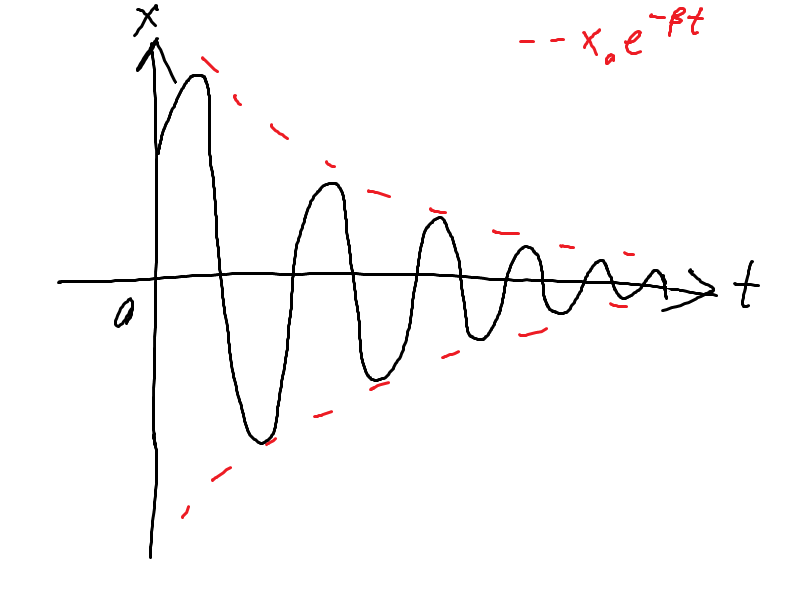
\includegraphics[width=0.33\linewidth]{fig/under-dump.png}
\caption{欠阻尼时的运动}
\label{fig-under-dump}
\end{figure}

$\beta$比较大时,$\Delta<0$,$\omega=\rmi \beta \pm \rmi \sqrt{\beta^2-\omega_0^2}$。根据解的线性叠加可以得到$x=A \rme^{\rmi (\rmi \beta+\rmi \sqrt{\beta^2-\omega_0^2}) t}+B \rme^{\rmi (\rmi \beta-\rmi \sqrt{\beta^2-\omega_0^2}) t}=A \rme^{-(\beta+\sqrt{\beta^2-\omega_0^2})t}+B \rme^{-(\beta-\sqrt{\beta^2-\omega_0^2})t}$。这种情况叫作过阻尼,小球的运动是两个指数衰减的叠加,而$A$和$B$要求都是实数。

$\beta$刚好不大不小时,$\Delta=0$,$\omega=\rmi \beta$,这种情况叫作临界阻尼。奇怪的事情出现了:二阶微分方程的通解必须有两个待定的常量,现在$\omega$只有一个解,怎么办?

我们要把猜解的形式换一下:$x=(A+B t)\rme^{-\beta t}$,代入微分方程,经过一坨求导和合并同类项得到$(A+B t)\rme^{-\beta t} (\omega_0^2-\beta^2)=0$,所以我们猜出来的这个解确实满足原方程,而且只有在临界阻尼的情况下才能这么猜解。到这里为止这个方程就解完了。

如果$\beta=0$,那么欠阻尼和过阻尼的运动都会变成简谐振动,而临界阻尼的运动会变成匀速直线运动。

要注意的是,指数衰减不能严格达到零,实际操作中一般认为小于一个很小的数(比如初始位移的1\%)就算运动停止,而且实际上的阻力也不严格与速度成正比。

【练习】自己把这个方程解一遍,如果能解出来那么之前的东西应该都懂了。
\section{受迫振动}
如果在弹簧振子上再加一个外力$f(t)=m a_0 \sin \omega t$,运动方程就是
\begin{equation*}
x''+2 \beta x'+\omega_0^2 x=a_0 \sin \omega t
\end{equation*}

这是一个非齐次方程,也就是说它的右边是有东西的。非齐次方程的困难之处就在于,没有一种通用的方法来猜解,需要根据方程右边的东西看着办。

通过物理实验我们已经知道,受迫振动的频率与外力相同,那么可以猜$x=A \sin \omega t+B \cos \omega t$,$A,B$都是实常量。代入方程得到
\begin{align*}
-\omega^2 A \sin \omega t-\omega^2 B \cos \omega t+2 \beta \omega (A \cos \omega t-B \sin \omega t)+\omega_0^2 (A \sin \omega t+B \cos \omega t)&=a_0 \sin \omega t \\
((\omega_0^2-\omega ^2)A-2 \beta \omega B)\sin \omega t +(2 \beta \omega A+(\omega ^2+\omega_0^2)B)\cos \omega t&=a_0 \sin \omega t
\end{align*}
\begin{equation*}
\begin{cases}
(\omega_0^2-\omega ^2)A-2 \beta \omega B=a_0 \\
2 \beta \omega A+(\omega ^2+\omega_0^2)B=0
\end{cases}
\end{equation*}

解得$A=\frac{(\omega_0^2-\omega ^2) a_0}{(\omega_0^2-\omega ^2)^2+(2 \beta \omega)^2}$,$B=\frac{2 \beta \omega a_0}{(\omega_0^2-\omega ^2)^2+(2 \beta \omega)^2}$,总振幅为$\sqrt{A^2+B^2}=\frac{a_0}{\sqrt{(\omega_0^2-\omega ^2)^2+(2 \beta \omega)^2}}$。根号里是$\omega$的二次函数,$\omega$略小于$\omega_0$时,振幅最大。相位的变化比较复杂,有(mei)兴(shi)趣(gan)的同学可以画个图。

但是!我们怎么把常量$A$和$B$解出来了?这里的$A$和$B$并不是待定常量,我们解出的只是一个特解,而不是通解。但是我们发现,如果$x_1(t)$是非齐次方程$x''+2 \beta x'+\omega_0^2 x=f(t)$的解,而$x_2(t)$是对应的齐次方程$x''+2 \beta x'+\omega_0^2 x=0$的解,那么$x_1(t)+x_2(t)$是这个非齐次方程的解。

所以把阻尼振动的通解加上去就是受迫振动的通解。阻尼振动的解会指数衰减,所以经过足够长的时间之后就只剩下受迫振动的特解。

【练习】解方程$x''+2 \beta x'+\omega_0^2 x=b_0 \rme^{-\lambda t}$,想一想应该猜什么样的解。

$\phantom{\text{【练习】}}$解方程$x''+2 \beta x'+\omega_0^2 x=a_0 \sin \omega t+b_0 \rme^{-\lambda t}$。真的要从头开始解一遍吗?
\section{小球、磁场与弹簧}
考虑这样一个问题:在平面内,一个小球质量为$m$,带电$q$,在一个匀强磁场$B$里,并且连着一根弹簧,劲度系数为$k$,忽略原长。把小球的坐标设为$(x,y)$,并且设$z=x+\rmi y$,小球的运动方程可以写成
\begin{equation*}
z''+2 \rmi \beta z'+\omega_0^2 z=0
\end{equation*}

其中$2 \beta=\frac{B q}{m}$,$\omega_0^2=\frac{k}{m}$。洛伦兹力的方向垂直于速度方向,所以$\beta$前面乘了一个$\rmi$。复数只要用乘法就可以表示旋转,所以二维问题经常要旋转某个东西就可以考虑用复数。

按照阻尼振动的解法,这个方程的解是$z=A \rme^{\rmi (-\beta+\sqrt{\beta^2+\omega_0^2}) t}+B \rme^{\rmi (-\beta-\sqrt{\beta^2+\omega_0^2}) t}$,其中$A$和$B$是复常量。也就是说,小球的运动是两个半径和角速度不同的圆周运动的叠加。

到现在为止讲的你可以当作全是扯蛋,至少没有哪个学校的自主招生会直接让你算微积分,但是微积分作为一种处理问题的思想是需要掌握的,这样就不需要苦逼的微元法了。
\section{睡前小故事:解方程有多复杂}
二元一次方程组解起来很简单,三元一次方程组就比较困难了,四元以上的方程组如果暴算的话一般是没有希望的,需要观察方程的特点才能解出来。我们可以想办法描述一下解方程的复杂程度。考虑一个$n$元一次方程组:
\begin{align*}
a_{1 1} x_1+a_{1 2} x_2+\dots+a_{1 n} x_n&=c_1 \\
a_{2 1} x_1+a_{2 2} x_2+\dots+a_{2 n} x_n&=c_2 \\
&\dots \\
a_{n 1} x_1+a_{n 2} x_2+\dots+a_{n n} x_n&=c_n
\end{align*}

假设你用一台很慢的电脑来解方程,它每秒可以算一次加法、减法、乘法或者除法。

首先用第一个方程表示出$x_1$:$x_1=\frac{c_1}{a_1}-\frac{a_2}{a_1} x_2-\frac{a_3}{a_1} x_3-\dots-\frac{a_n}{a_1} x_n$。每算一次$\frac{c_1}{a_1}$之类的系数要1秒,总共要$n$秒。

然后把$x_1$代入到第二个方程,这样$x_2$的系数就变成了$-a_{2 1} \frac{a_2}{a_1}+a_{2 2}$,算一次乘法一次加法要2秒,算$n-1$个$x$的系数要$2n-2$秒。

把$x_1$代入到后面的$n-1$个方程里总共要$(2n-2)(n-1)=2n^2-4n+2$秒,加上前面的$n$秒是$2n^2-3n+2$秒。这样$x_1$就从整个方程组里消掉了,剩下$n-1$元一次方程组。

这样的步骤要进行$n$次,总共需要$\sum_{i=1}^n(2i^2-3i+2)=\frac{2}{3} n^3-\frac{1}{2} n^2+\frac{5}{6} n$秒。现在终于解出了一个$x_n$,然后要把它代到上面的式子里解出其他$x$,但是先不管这个。

现在的电脑可以解成千上万个方程联立的方程组。当$n$很大的时候,可以不管一次和二次项,甚至不管三次项的系数$\frac{2}{3}$,所以说$\frac{2}{3} n^3-\frac{1}{2} n^2+\frac{5}{6} n$是一个复杂度为$O(n^3)$的函数。

举几个栗子,$x^3+2x^2+3x$和$4x^3+\frac{5}{x}+6 \sin x$都是$O(x^3)$的函数。当$x$很大的时候,$O(x^3)$的增长速度远大于$O(n^2)$。

$\exp x$的增长速度比任何$x^a$($a$为正数)都大,而$\ln x$的增长速度比任何$x^a$都小。$x^x$的增长速度比$\exp x$还大。

复杂度理论可以帮我们优化做一些事情的方法。比如计算多项式$P(x)=a_0+a_1 x+a_2 x^2+\dots+a_n x^n$,如果一项一项算,第一项是常数,第二项需要一次乘法,第三项需要两次乘法……最后一项需要$n$次乘法,加起来需要$n$次加法,总共需要$\frac{1}{2} n^2+\frac{3}{2} n$秒,复杂度为$O(n^2)$。

但是如果这样算:$P(x)=a_0+x (a_1+x (a^2+\dots))$,那么只需要$2 n$秒,复杂度为$O(n)$。也就是说,把$x^a$记下来,下次要算$x^{a+1}$只要乘一次$x$,而不用从头开始乘。这种方法叫作\emph{秦九韶算法},在国外则叫\emph{霍纳算法}。

一件事情的复杂度是对给定的基本操作而言的,如果你有一台牛逼的电脑可以在一秒钟内算一个多项式,那当我没说。

\chapter{线性代数}
\section{矩阵;矩阵的加法、减法、数乘}
矩阵就是把一些东西排成方形,这些东西可以是实数,也可以是复数或者函数之类的。比如矩阵$\mathbf{A}=\begin{bmatrix}
1 & 2 & 3 \\
4 & 5 & 6
\end{bmatrix}$,它有$2$行$3$列。我们用黑体字母表示矩阵。$A_{i j}$表示$i$行$j$列的元素,比如$A_{1 3}=3$,$A_{2 2}=5$。有时候下标未知的$A_{i j}$也可以表示整个矩阵。

行数与列数各自相同的矩阵可以加减,只要把对应的元素加减就行了。比如$\mathbf{B}=\begin{bmatrix}
2 & 3 & 3 \\
6 & 6 & 6
\end{bmatrix}$,那么$\mathbf{A}+\mathbf{B}=\begin{bmatrix}
3 & 5 & 6 \\
10 & 11 & 12
\end{bmatrix}$。

矩阵还可以与一个数(实数或复数)相乘,叫作数乘,只要把对应的元素与这个数相乘就行了。比如$2 \mathbf{A}=\begin{bmatrix}
2 & 4 & 6 \\
8 & 10 & 12
\end{bmatrix}$。一般把数写在矩阵的前面,中间不写$\cdot$或$\times$等符号。

矩阵还有一种运算叫作转置,就是把它沿着对角线翻过来,行变成列,列变成行。矩阵$\mathbf{A}$的转置用$\mathbf{A}^\opT$表示,$A^\opT_{i, j}=A_{j, i}$。比如上面的$\mathbf{A}=\begin{bmatrix}
1 & 2 & 3 \\
4 & 5 & 6
\end{bmatrix}$,那么$\mathbf{A}^\opT=\begin{bmatrix}
1 & 4 \\
2 & 5 \\
3 & 6
\end{bmatrix}$。

矢量也是一种矩阵,它只有一行或者一列,一般用一列来表示,需要的时候可以转置。$A_i$表示矢量$A$的第$i$个元素。标量也是一种矩阵,它只有一行和一列。
\section{矩阵乘法;坐标变换;爱因斯坦求和约定}
矩阵和矩阵也可以相乘,但是要复杂一些。我们定义:如果$\mathbf{A} \mathbf{B}=\mathbf{C}$,那么$C_{i k}=\sum_j A_{i j} B_{j k}$。只有$\mathbf{A}$的列数与$\mathbf{B}$的行数相同才能相乘,求和的时候$j$的取值范围是$\mathbf{A}$的列数,也是$\mathbf{B}$的行数。

比如$\mathbf{A}=\begin{bmatrix}
1 & 2 \\
3 & 4
\end{bmatrix}$,$\mathbf{B}=\begin{bmatrix}
5 & 6 \\
7 & 8
\end{bmatrix}$,那么$\mathbf{A} \mathbf{B}=\begin{bmatrix}
1 \times 5+2 \times 7 & 1 \times 6+2 \times 8 \\
3 \times 5+4 \times 7 & 3 \times 6+4 \times 8
\end{bmatrix}=\begin{bmatrix}
19 & 22 \\
43 & 50
\end{bmatrix}$。

一般情况下矩阵乘法不满足交换律。比如$\mathbf{B} \mathbf{A}=\begin{bmatrix}
5 \times 1+6 \times 3 & 5 \times 2+6 \times 4 \\
7 \times 1+8 \times 3 & 7 \times 2+8 \times 4
\end{bmatrix}=\begin{bmatrix}
23 & 34 \\
31 & 46
\end{bmatrix} \neq \mathbf{A} \mathbf{B}$。如果行数和列数不合适,交换之后的矩阵乘法甚至可能没有意义。但是矩阵乘法满足结合律,你可以自己验证这一点。

为什么会有这么奇怪的定义呢?先来看一个例子:如图\ref{fig-rotate},在平面直角坐标系$O-x-y$中,点$P$的坐标是$(x_P, y_P)$。现在把点$P$(注意不是坐标轴)绕$O$逆时针旋转角度$\theta$,得到点$P'$。容易算出$x_{P'}=x_P \cos \theta-y_P \sin \theta$,$y_{P'}=x_P \sin \theta+y_P \cos \theta$。
\begin{figure}[htb]
\centering
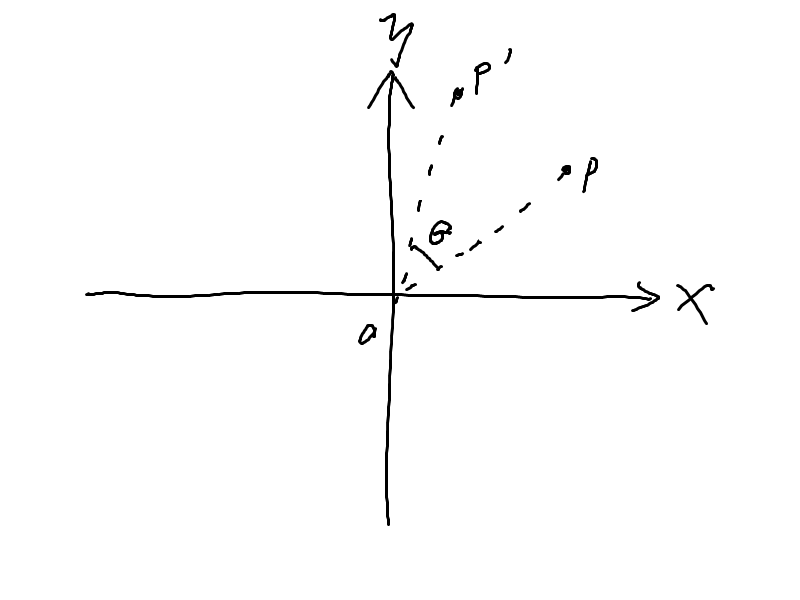
\includegraphics[width=0.33\linewidth]{fig/rotate.png}
\caption{把$OP$转过去}
\label{fig-rotate}
\end{figure}

如果用矢量$\mathbf{P}=\begin{bmatrix} x_p \\ y_p \end{bmatrix}$表示$P$的坐标,矩阵$\mathbf{R}(\theta)=\begin{bmatrix}
\cos \theta & -\sin \theta \\
\sin \theta & \cos \theta
\end{bmatrix}$表示旋转操作(它的元素是$\theta$的函数),那么$P$的坐标$\mathbf{P'}=\mathbf{R}(\theta) \mathbf{P}$,这样看起来就比较厉害。

【练习】证明$\mathbf{R}(\alpha) \mathbf{R}(\beta)=\mathbf{R}(\alpha+\beta)$。

矩阵不但可以表示旋转,还可以表示缩放。比如$\mathbf{S}=\begin{bmatrix}
2 & 0 \\
0 & 1
\end{bmatrix}$就表示把$x$坐标放大到原来的$2$倍,而$y$坐标不变。

如果把$P$旋转$\theta$角,再把$x$坐标放大到$2$倍,然后旋转$\phi$角得到$P'$,只要依次把矩阵从右到左乘起来就行了,也就是$\mathbf{P'}=\mathbf{R}(\phi) \mathbf{S} \mathbf{R}(\theta) \mathbf{P}$。这样就能直观地看出矩阵乘法不满足交换律。(从右到左写的习惯和我们熟悉的函数一样,比如$f_2(f_1(x))$表示对$x$先进行$f_1$这个操作,再进行$f_2$这个操作)

日常生活中有许多东西不满足交换律,比如你爸爸的妈妈和你妈妈的爸爸不是同一个人,再比如三维空间中先向左转$90$度,再向上转$90$度与先向上转$90$度,再向左转$90$度是不一样的。这样的东西在数学上称为\emph{非阿贝尔群}。

【练习】$\mathbf{A}=\begin{bmatrix}
0 & 1 & 0 & 0 \\
1 & 0 & 0 & 0 \\
0 & 0 & 1 & 0 \\
0 & 0 & 0 & 1
\end{bmatrix}$,$\mathbf{B}=\begin{bmatrix}
1 & 2 & 3 & 4 \\
5 & 6 & 7 & 8 \\
9 & 10 & 11 & 12 \\
13 & 14 & 15 & 16
\end{bmatrix}$,求$\mathbf{A} \mathbf{B}$和$\mathbf{B} \mathbf{A}$。$\mathbf{A}$乘在左边和右边分别表示什么操作?

在计算矩阵乘法时经常出现求和号。有一天爱因斯坦说:两个矩阵相乘,如果有相同的下标就表示求和,求和号可以不写。比如$C_{i k}=\sum_j A_{i j} B_{j k}$可以写成$C_{i k}=A_{i j} B_{j k}$,而$\mathbf{P'}=\mathbf{R}(\phi) \mathbf{S} \mathbf{R}(\theta) \mathbf{P}$可以写成$P'_i=R_{i j}(\phi) S_{j k} R_{k l}(\theta) P_l$。如果没有相同的指标就不表示求和,比如$A_i$是一个$m$列的矢量,$B_i$是一个$n$列的矢量,$C_{i j}=A_i B_j$,那么$C_{i j}$就是一个$m$行$n$列的矩阵。

(用什么字母作为下标不会影响矩阵的内容,比如$A_{i j}$和$A_{k l}$表示的是同一个矩阵)
\section{对矩阵求导}
在平面上的一个静止的参考系$S$中,有一个矢量$\mathbf{A}$,它可以随着时间变化。在以角速度$\omega$顺时针旋转的参考系$S'$中看,得到$\mathbf{A'}=\mathbf{R} \mathbf{A}$,其中$\mathbf{R}=\begin{bmatrix}
\cos \omega t & -\sin \omega t \\
\sin \omega t & \cos \omega t
\end{bmatrix}$,它也是时间$t$的函数。

现在来看$S'$系中$\mathbf{A'}$的速度:$\frac{\opd \mathbf{A'}}{\opd t}=\frac{\opd \mathbf{R}}{\opd t} \mathbf{A}+\mathbf{R} \frac{\opd \mathbf{A}}{\opd t}$。

对两个矩阵的乘积求导,跟对两个数的乘积求导是一样的,因为计算导数的时候没有用到乘法交换律。容易理解,$\mathbf{R} \frac{\opd \mathbf{A}}{\opd t}$就是把$S$系中$\mathbf{A}$的速度用$\mathbf{R}$旋转一下。但是$\frac{\opd \mathbf{R}}{\opd t} \mathbf{A}$是什么意思呢?

我们直接计算$\frac{\opd \mathbf{R}}{\opd t}=\begin{bmatrix}
-\sin \omega & -\cos \omega \\
\cos \omega & -\sin \omega
\end{bmatrix}$,也就是对矩阵中的每个元素分别求导。然后计算$\frac{\opd \mathbf{R}}{\opd t} \mathbf{A}$就会发现,它是一个矢量,大小为$\omega A$,方向为$\mathbf{A}$逆时针转$90$度,相当于旋转引起的线速度。

也可以用直观的几何方法来理解,如图\ref{fig-rotate-deri},$\frac{\opd \mathbf{R}}{\opd t} \mathbf{A}=\frac{1}{\opd t}(\mathbf{R}(t+\opd t) \mathbf{A}-\mathbf{R}(t) \mathbf{A})$,当$\opd t$无限小时,它的方向垂直于$\mathbf{A}$。
\begin{figure}[htb]
\centering
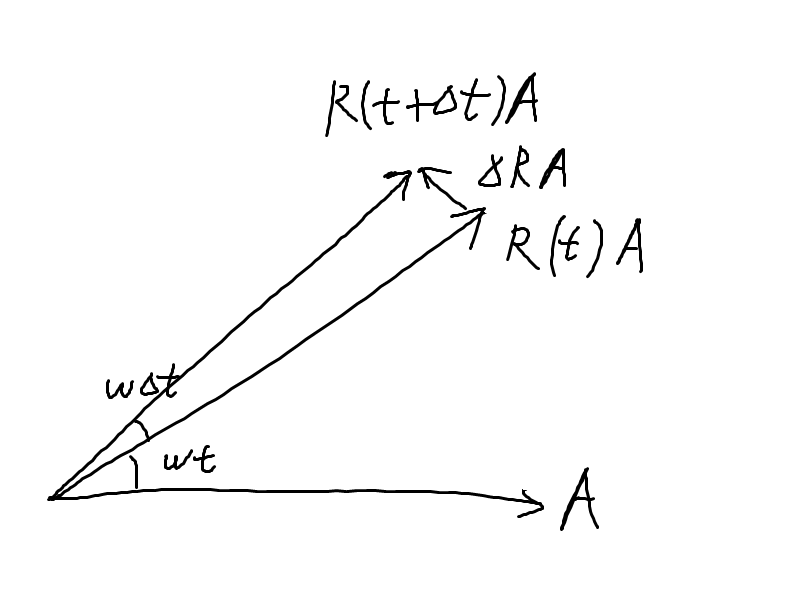
\includegraphics[width=0.33\linewidth]{fig/rotate-deri.png}
\caption{把$\mathbf{A}$转过去}
\label{fig-rotate-deri}
\end{figure}

(用类似的方法可以求$A'$的加速度,但是理解起来比较麻烦,以后再讲)
\section{零矩阵;单位矩阵;逆矩阵}
零矩阵$\mathbf{0}$就是$\begin{bmatrix}
0 & 0 & \dots & 0 \\
0 & 0 & \dots & 0 \\
\vdots & \vdots & \ddots & \vdots \\
0 & 0 & \dots & 0
\end{bmatrix}$这样的矩阵。它的行数与列数是多少可以根据上下文判断。一个矩阵跟(大小合适的)$\mathbf{0}$相加,得到的矩阵与原来一样;跟$\mathbf{0}$相乘(不管在左边还是右边),得到$\mathbf{0}$。

单位矩阵$\mathbf{I}$就是$\begin{bmatrix}
1 & 0 & \dots & 0 \\
0 & 1 & \dots & 0 \\
\vdots & \vdots & \ddots & \vdots \\
0 & 0 & \dots & 1
\end{bmatrix}$这样的矩阵。一般认为它的行数与列数相同,具体是多少也要根据上下文判断。一个矩阵跟$\mathbf{I}$相乘,得到的矩阵与原来一样。

如果两个矩阵$\mathbf{A}$和$\mathbf{A'}$相乘得到$\mathbf{I}$,那么$\mathbf{A}$和$\mathbf{A'}$互为逆矩阵。如果$\mathbf{A'} \mathbf{B}=\mathbf{C}$,那么在$\mathbf{C}$前面再乘一个$\mathbf{A}$又得到了$\mathbf{B}$(别忘了矩阵乘法满足结合律),就像是除以$\mathbf{A'}$一样。

然而不是每个矩阵都存在逆矩阵,即使逆矩阵存在,从$\mathbf{A}$算出$\mathbf{A'}$也比较麻烦。一种容易理解但是不容易算的方法是待定系数法,更好的方法需要利用行列式的性质,我们以后再讲。逆矩阵有许多实际应用,在各种实际情况下快速计算逆矩阵是一个热门的问题。

【练习】证明$\begin{bmatrix}
1 & 2 \\
3 & 4
\end{bmatrix}$的逆矩阵是$\begin{bmatrix}
-2 & 1 \\
\frac{3}{2} & -\frac{1}{2}
\end{bmatrix}$。
\section{行列式;坐标系的手性}
行数和列数相同的矩阵叫作方阵,它的行数或者列数也可以叫作阶数。行列式是一个把方阵变成实数的操作,矩阵$\mathbf{A}$的行列式用$\det \mathbf{A}$或者$|\mathbf{A}|$表示。(行列式的绝对值用$||\mathbf{A}||$表示)

二阶行列式$\begin{vmatrix}
a & b \\
c & d
\end{vmatrix}=a d-b c$,三阶行列式$\begin{vmatrix}
a & b & c \\
d & e & f \\
g & h & i
\end{vmatrix}=a e i+b f g+c d h-c e g-a f h-b d i$(找一找这个式子的规律)。更高阶的行列式计算比较麻烦,而且不常用,我们待会再讲。

这个东西有什么用呢?在二维平面内,如果点$P(x_P, y_P), Q(x_Q, y_Q)$,那么$S_{\triangle O P Q}=\frac{1}{2}\begin{vmatrix}
x_P & y_P \\
x_Q & y_Q
\end{vmatrix}$。你可以用解析几何验证一下。这就是传说中的叉积$\mathbf{P} \times \mathbf{Q}$的二维形式。

(顺便说一句,二维矢量的叉积是一个标量,三维矢量的叉积是一个矢量,更高维度的叉积以后再讲。)

这个“面积”算出来有可能是负的,因为$P$和$Q$在行列式中的位置不一样。可以用右手螺旋来判断:把右手四指指向$O P$方向,然后转向$O Q$方向。如果大拇指朝上,那么就是正的,否则就是负的。高考范围内一般只要取绝对值就行了。算三角形面积别忘了乘$\frac{1}{2}$。

在三维空间内,如果点$P(x_P, y_P, z_P), Q(x_Q, y_Q, z_Q), R(x_R, y_R, z_R)$,那么三棱锥$O-P Q R$的体积$V=\frac{1}{6}\begin{vmatrix}
x_P & y_P & z_P \\
x_Q & y_Q & z_Q \\
x_R & y_R & z_R
\end{vmatrix}$。这样可以秒杀一些立体几何题。这个“体积”也有可能是负的,记得取绝对值。

如果把矩阵看作一个坐标变换,那么行列式就是坐标变换之后和之前的图形的体积(不管几维都叫体积好了)之比。比如二维情况下,设矩阵$\mathbf{A}=\begin{bmatrix}
a & b \\
c & d
\end{bmatrix}$是一个坐标变换,点$\mathbf{P}=\begin{bmatrix} 1 \\ 0 \end{bmatrix}$,$\mathbf{Q}=\begin{bmatrix} 0 \\ 1 \end{bmatrix}$,$\mathbf{P'}=\mathbf{A} \mathbf{P}=\begin{bmatrix} a \\ c \end{bmatrix}$(这里不严格区分点和它对应的矢量),$\mathbf{Q'}=\mathbf{A} \mathbf{Q}=\begin{bmatrix} b \\ d \end{bmatrix}$,那么$S_{\triangle O P Q}=\frac{1}{2}(a d-b c)$。只要对单位三角形$\triangle O P Q$验证了这一点,由面积的可加性,这一点对任意图形都是成立的。

如果这个“体积”之比是负的,说明这个坐标变换改变了坐标系的\emph{手性}。不管在几维空间内,都存在着两种手性的坐标系,我们一般习惯用右手系。比如二维情况下,坐标变换$\begin{bmatrix}
-1 & 0 \\
0 & 1
\end{bmatrix}$把$x$轴反过来(专业一点叫\emph{空间反演变换}),$y$轴不变,那么坐标系的手性就改变了。同时反转$x$轴和$y$轴不会改变坐标系的手性,旋转变换也不会。

如果$\mathbf{A}$是$n$维矩阵,$c$是实数,那么$|c \mathbf{A}|=c^n |\mathbf{A}|$。矩阵乘法可以表示两次连续的坐标变换,所以$|\mathbf{A} \mathbf{B}|=|\mathbf{A}| |\mathbf{B}|$。如果方阵的一行或者一列全是$0$,那么行列式就是$0$。

行列式只是一种数学工具,图形的体积和变换的体积之比是它的两种应用,在其他地方还会遇到类似的式子。
\section{用行列式解线性方程组}
现在用看起来很厉害的方法解二元一次方程组
\begin{equation*}
\begin{cases}
a_{1 1} x_1+a_{1 2} x_2=b_1 \\
a_{2 1} x_1+a_{2 2} x_2=b_2 \\
\end{cases}
\end{equation*}

如果$b_1, b_2$不全为$0$,先设$D=\begin{vmatrix}
a_{1 1} & a_{1 2} \\
a_{2 1} & a_{2 2}
\end{vmatrix}$。如果$D \neq 0$,我们说这两个方程线性无关(也就是独立),可以解出$x_1=\frac{1}{D}\begin{vmatrix}
a_{1 1} & b_1 \\
a_{2 1} & b_2
\end{vmatrix}$,$x_2=\frac{1}{D}\begin{vmatrix}
a_{1 2} & b_1 \\
a_{2 2} & b_2
\end{vmatrix}$。你可以用消元法暴算出方程的解,然后比较一下。如果两种方法都很熟悉,运算量是差不多的。

如果$D=0$,说明方程组无解或者有无穷多个解,具体是哪种情况要解解看才知道。我们说这两个方程线性相关,也就是说它们乘一个倍数可以变成同一个方程。

如果$b_1=b_2=0$,也就是说这是一个齐次方程组。如果$D \neq 0$,用上面的方法算出$x_1=x_2=0$,这确实是一个解,但是没有非零解,也就是说矢量$(a_{1 1}, a_{2 1})$和$(a_{1 2}, a_{2 2})$不共线。如果$D=0$,有无穷多个解。

类似的方法可以解三元或者更多元的线性方程组,以及判断三维空间中矢量的共面情况。这些事情的严格证明一般是先证明二阶的情况,再用归纳法证明更高阶的情况。
\section{高阶行列式}
(这部分内容看不懂可以先跳过,有兴趣的同学可以去看线性代数的书)

首先定义$P_i$是自然数$1, 2, 3, \dots, n$的一个排列,称为$n$阶排列。比如$(2, 1, 3, 4, 5), (5, 4, 3, 2, 1)$都是$5$阶排列。不同的下标$i$表示不同的排列,而不是排列中的第$i$个元素。

然后定义一个操作叫置换,就是把排列里的两个数换一下。比如$5$阶排列$(1, 2, 3, 4, 5)$经过置换可以得到$(2, 1, 3, 4, 5)$,再置换一次可以得到$(2, 3, 1, 4, 5)$等等。任何一个$n$阶排列都可以从$(1, 2, 3, \dots, n)$经过置换得到。

我们要把所有排列分成两类:奇排列和偶排列。设$(1, 2, 3, \dots, n)$至少经过$m$次置换才能得到$P_i$,如果$m$是奇数,$P_i$就是奇排列,否则是偶排列。

接着定义一个正负号函数$sgn(P_i)$:如果$P_i$是奇排列,那么$sgn(P_i)=+1$,否则$sgn(P_i)=-1$。

现在可以定义$n$阶方阵$\mathbf{A}$的行列式
\begin{equation*}
|\mathbf{A}|=\sum_{P_i} sgn(P_i) \prod_{k=1}^n A_{k P_k}
\end{equation*}

其中求和是对所有$n$阶排列$P_i$求和,$\prod$表示连乘。比如$n=5$时,共有$120$个排列,其中有一个是$P_i=(2, 3, 1, 4, 5)$,它是偶排列,那么求和号里就有一项$-A_{1 2} A_{2 3} A_{3 1} A_{4 4} A_{5 5}$。把$120$项加起来就得到了行列式的值。你可以验证一下前面说的二阶和三阶行列式符合这样的定义。

这是行列式的一种定义,但是真的用这种方法计算是很麻烦的。$n$阶排列共有$n!$个,所以这种方法的复杂度是$O(n!)$。我们已经知道可以用行列式解线性方程组,而解线性方程组有$O(n^3)$的方法,那么算行列式肯定也有$O(n^3)$的方法,称为\emph{高斯消元法}。行列式还有许多运算技巧,我们以后再讲。
\section{矩阵的幂;矩阵级数}
定义了矩阵乘法之后就可以定义幂运算。比如$\mathbf{A}^2=\mathbf{A} \mathbf{A}$。但是矩阵的幂运算并不常用,只有矩阵是方阵,并且指数是整数的时候才有意义。矩阵乘法不满足交换律,所以$(\mathbf{A} \mathbf{B})^2=\mathbf{A}^2 \mathbf{B}^2$这样的公式也不成立。

如果把一个函数表示成级数,它的定义域和值域可以都是矩阵。比如
\begin{equation*}
\rme^\mathbf{A}=\sum_{n=0}^{\infty}\frac{1}{n!}\mathbf{A}^n=1+\mathbf{A}+\frac{1}{2}\mathbf{A}^2+\frac{1}{6}\mathbf{A}^3+\dots
\end{equation*}

这样一来,线性微分方程组
\begin{align*}
\opdt x_1 &=a_{1 1} x_1+a_{1 2} x_2+\dots+a_{1 n} x_n \\
\opdt x_2 &=a_{2 1} x_1+a_{2 2} x_2+\dots+a_{2 n} x_n \\
&\dots \\
\opdt x_2 &=a_{n 1} x_1+a_{n 2} x_2+\dots+a_{n n} x_n
\end{align*}

可以直接写成$\opdt \mathbf{x}=\mathbf{a} \mathbf{x}$,它的解就是$\mathbf{x}=\rme^{t \mathbf{a}} \mathbf{x_0}$。(注意字母相乘的顺序,解微分方程的时候并没有用到乘法交换律)

$\mathbf{x_0}$表示初始条件,而$\rme^{t \mathbf{a}}$表示系统随着时间演化的规律。不管初始条件是什么,演化的规律总是相同的。然而要计算出矩阵函数的值,并不是一件容易的事情。
\section{线性空间}
实数、复数、矢量和矩阵有一些共同点,比如都能进行加法和数乘运算,这样的集合叫作线性空间。

严格来说,线性空间的定义是这样的:设$V$是一个集合,$a, b, c$是它的元素,$\lambda, \mu$是数。定义一种加法运算把两个元素变成一个元素,数乘运算把一个数和一个元素变成一个元素,它们满足:
\begin{enumerate}
\item $(a+b)+c=a+(b+c)$。
\item $a+b=b+a$。
\item 存在一个元素$0$,对任何元素$a$,$a+0=a$。(其实这句话中的“一个”不是必须的)
\item 对任何元素$a$,存在一个元素$-a$,$a+(-a)=0$。
\item $1 a=a$。
\item $(\lambda \mu) a=\lambda (\mu a)$。
\item $(\lambda+\mu) a=\lambda a +\mu a$。
\item $\lambda (a+b)=\lambda a +\lambda b$。
\end{enumerate}

(更抽象的定义中$\lambda$不一定是数,可以是其他奇怪的东西,关于数域的事情以后再讲。)

实数集$R$和复数集$C$都是线性空间。行数为$m$,列数为$n$的所有矩阵组成的集合$M(m, n)$也是线性空间。如果一个公式里只出现加法和数乘运算,那么不管里面的字母属于什么线性空间,都可以把公式套上去用。比如$F=m a$中的$F$和$a$有时候理解成实数,有时候理解成矢量。

以后讲量子力学的时候会用到这些东西,讲傅立叶变换的时候还会用到。

\chapter{矢量分析}
\section{nabla算符$\nabla$;梯度;散度;旋度;张量积}
这一章与矢量和微积分有关,以后讲电动力学的时候会用到。你可以想一想电磁学中的例子,还可以用软件画一些矢量场试试看。

首先要讲一个符号$\nabla$读作nabla。(也有人会读成del,还有些地方叫作哈密顿算符,但是这样会跟量子力学中的哈密顿算符搞混)它既是矢量,又是算符。在三维直角坐标系中,$\nabla=(\ppx,\ppy,\ppz)$。简单起见,接下来遇到的大多是二维的情况。

$\nabla$可以作用到标量或者矢量上面。把它作用到标量$f$上面,会变成一个矢量:$\nabla f=(\frac{\partial f}{\partial x},\frac{\partial f}{\partial y},\frac{\partial f}{\partial z})$,称为$f$的梯度。

如果$f$是$x,y,z$的函数,相当于在空间中的每个点都有一个$f$的值,我们说$f$是一个标量场。同样,空间中的每个点都有一个矢量$\nabla f$,我们说$\nabla f$是一个矢量场。

举个栗子:$f=x^2+y$,$\nabla f=(2x,1,0)$,如图\ref{fig-vec-grad},越白的地方$f$越大。
\begin{figure}[htb]
\centering
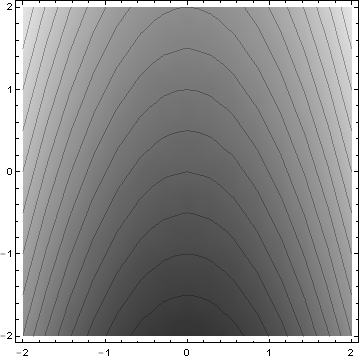
\includegraphics[width=0.33\linewidth]{fig/vec-grad.png}
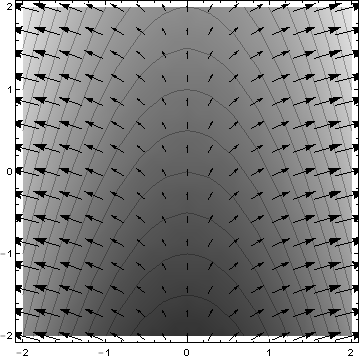
\includegraphics[width=0.33\linewidth]{fig/vec-grad-2.png}
\caption{沿着箭头爬上去}
\label{fig-vec-grad}
\end{figure}

$\nabla f$表示$f$变化的快慢和方向。比如$f$是电势,$-\nabla f$就是电场。

如果把$\nabla$作用到矢量上面,一般有三种方法:点积,叉积,张量积。$\nabla$与矢量$\mathbf{A}$点积,会变成一个标量:$\nabla \cdot \mathbf{A}=\frac{\partial A_x}{\partial x}+\frac{\partial A_y}{\partial y}+\frac{\partial A_z}{\partial z}$,称为$\mathbf{A}$的散度。

举个栗子:$\mathbf{A}=(1-x^2,y,0)$,$\nabla \cdot \mathbf{A}=1-2x$,如图\ref{fig-vec-div},越白的地方$\nabla \cdot \mathbf{A}$越大。
\begin{figure}[htb]
\centering
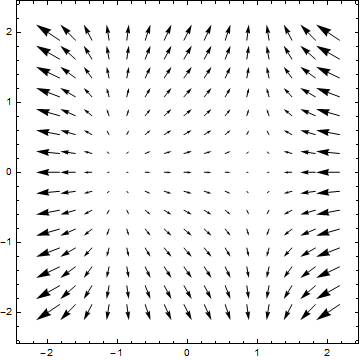
\includegraphics[width=0.33\linewidth]{fig/vec-div.png}
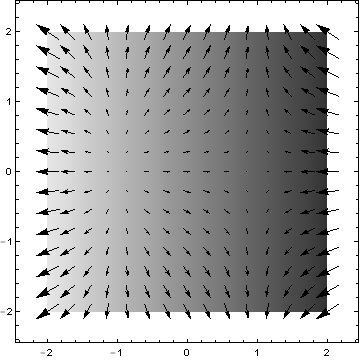
\includegraphics[width=0.33\linewidth]{fig/vec-div-2.png}
\caption{箭头出来了又进去了}
\label{fig-vec-div}
\end{figure}

$\nabla \cdot \mathbf{A}$表示$\mathbf{A}$在某个点上变多的程度,负数则表示变少。图\ref{fig-vec-div}的左边比较白,$\nabla \cdot \mathbf{A}>0$,可以看到从某个点出来的箭头比进去的大;右边比较黑,$\nabla \cdot \mathbf{A}<0$,进去的箭头比出来的大。

比如正的点电荷上面的$\nabla \cdot \mathbf{E}>0$,没有电荷的地方$\nabla \cdot \mathbf{E}=0$。如果一条河里的水流速度为$\mathbf{v}$,即使我们不知道水是怎么流的,但是任何一个点进去和出来的水肯定一样多,所以$\nabla \cdot \mathbf{v}=0$。

$\nabla$与矢量$\mathbf{A}$叉积,仍然是一个矢量(背一遍叉积的公式):$\nabla \times \mathbf{A}=(\frac{\partial A_z}{\partial y}-\frac{\partial A_y}{\partial z},\frac{\partial A_x}{\partial z}-\frac{\partial A_z}{\partial x},\frac{\partial A_y}{\partial x}-\frac{\partial A_x}{\partial y})$,称为$\mathbf{A}$的旋度。

举个栗子:$\mathbf{A}=(-\frac{y}{x^2+y^2+1},\frac{x}{x^2+y^2+1},0)$,$\nabla \times \mathbf{A}=(0,0,\frac{2}{(x^2+y^2+1)^2})$。因为$\mathbf{A}$只有$x,y$分量,所以$\nabla \times \mathbf{A}$只有$z$分量。如图\ref{fig-vec-curl},越白的地方$(\nabla \cdot \mathbf{A})_z$越大。
\begin{figure}[htb]
\centering
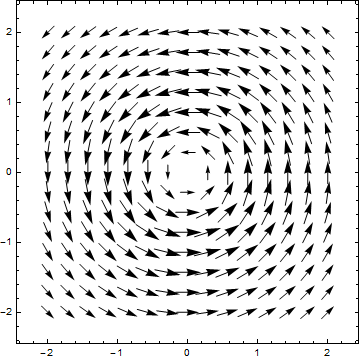
\includegraphics[width=0.33\linewidth]{fig/vec-curl.png}
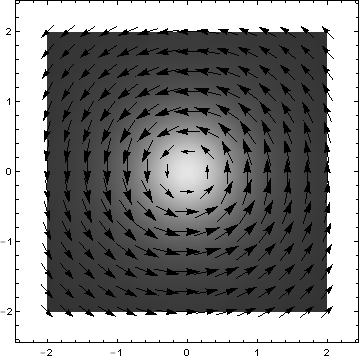
\includegraphics[width=0.33\linewidth]{fig/vec-curl-2.png}
\caption{高速旋转!面对疾风吧!!!!}
\label{fig-vec-curl}
\end{figure}

$\nabla \times \mathbf{A}$表示$\mathbf{A}$在某个点上旋转的程度,以及旋转的方向(用右手螺旋表示)。图\ref{fig-vec-curl}中的箭头全都在逆时针转,所以$\nabla \times \mathbf{A}$指向$+z$方向。比如电流$I$周围会形成一圈圈磁场,$\nabla \times \mathbf{B}$指向电流方向。

如果$\mathbf{A}$是匀强场,那么$\nabla \cdot \mathbf{A}=0$,$\nabla \times \mathbf{A}=\mathbf{0}$。

如果知道(空间中每个点的)$\nabla f$,通过积分就能确定$f$,最多相差一个积分常量。知道$\nabla \cdot \mathbf{A}$和$\nabla \times \mathbf{A}$,通过更复杂的积分也能确定$\mathbf{A}$,最多相差一个常矢量。

最后是$\nabla$与$\mathbf{A}$的张量积,一般写成$\nabla \mathbf{A}$,中间没有$\cdot$也没有$\times$。(虽然有些人会用各种奇怪的写法)它一般出现在运算的中间过程,至于物理意义就很难讲。它是一个$3 \times 3$的张量:
\begin{equation}
\nabla \mathbf{A}=\partial_i A_j=\begin{bmatrix}
\frac{\partial A_x}{\partial x} & \frac{\partial A_y}{\partial x} & \frac{\partial A_z}{\partial x} \\
\frac{\partial A_x}{\partial y} & \frac{\partial A_y}{\partial y} & \frac{\partial A_z}{\partial y} \\
\frac{\partial A_x}{\partial z} & \frac{\partial A_y}{\partial z} & \frac{\partial A_z}{\partial z}
\end{bmatrix}
\end{equation}

还要注意,在不同的坐标系中,$\nabla$的分量是不同的,不一定只有偏导数。简单起见,接下来遇到的都是直角坐标系。
\section{高斯定理;斯托克斯定理}
在三维空间中随便画一个闭合曲面$S$,可以计算矢量场$\mathbf{A}$在$S$上的通量$\Phi=\oint_S \mathbf{A} \cdot \opd \mathbf{S}$。

($\oint_S$表示对$S$上的每个小面元进行积分,圆圈表示闭合曲面,这只是书写的一些习惯。有些地方会写成$\oiint$,表示小面元是二维的。矢量$\opd \mathbf{S}$表示一个有方向的小面元,它的大小是小面元的面积,方向垂直于小面元向外)

把$S$里面的区域记为$V$,计算$\int_V \nabla \cdot \mathbf{A} \opd V$。既然$\nabla \cdot \mathbf{A}$表示$\mathbf{A}$在某个点上变多了多少,把它对$V$积分就是$\mathbf{A}$在$S$里面总共多了多少。这些多出来的$\mathbf{A}$会从$S$上出去,就是$\Phi$。这个公式称为高斯定理:
\begin{equation*}
\oint_S \mathbf{A} \cdot \opd \mathbf{S}=\int_V \nabla \cdot \mathbf{A} \opd V
\end{equation*}

举个栗子:如图\ref{fig-gauss-flux},$\mathbf{A}=(1-x^2,y,0)$,画一个三角形$\triangle ABC$,$A(0,0,0),B(1,0,0),C(0,1,0)$。验证一下高斯定理:

(简单起见,我们把三维问题变成二维问题,现在$S$是三角形的边,$V$是三角形里面的面积)
\begin{figure}[htb]
\centering
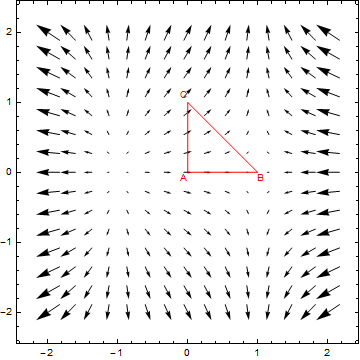
\includegraphics[width=0.33\linewidth]{fig/gauss-flux.png}
\caption{验证高斯定理}
\label{fig-gauss-flux}
\end{figure}
\begin{align*}
\nabla \cdot \mathbf{A}&=1-2 x \\
\int_V \nabla \cdot \mathbf{A} \opd V&=\int_{x=0}^1 \int_{y=0}^{1-x} (1-2 x) \opd x \opd y
\internote{(对面积积分可以对$x$和$y$分别积分。这里$y$的积分上限与$x$有关,所以要先对$y$积分,再对$x$积分)}
&=\int_0^1 \left( \int_0^{1-x} (1-2 x) \opd y \right) \opd x \\
&=\int_0^1 (1-x)(1-2 x) \opd x \\
&=\frac{1}{6}
\end{align*}

$\oint_S \mathbf{A} \cdot \opd \mathbf{S}$要在三条边上分开算。$AB$边上的$\mathbf{A}$平行于$AB$边,通量$\oint_{AB} \mathbf{A} \cdot \opd \mathbf{S}$显然是0。

$AC$边的单位法向量$\mathbf{n}_{AC}=(-1,0)$(注意要向外),$\mathbf{A} \cdot \mathbf{n}_{BC}|_{x=0}=-1$。$AC$边平行于$y$轴,$\opd \mathbf{S}$的大小就是$\opd y$。$\oint_{AC} \mathbf{A} \cdot \opd \mathbf{S}=\int_0^1 (-1) \opd y=-1$。

$BC$边是斜着的,所以会复杂一些。我们可以把它\emph{参数化}:定义一个参数$t$,它既表示$x$的变化,又表示$y$的变化。令$0<t<1$,$x=t$,$y=1-t$,$\opd S=\sqrt{(\opd x)^2+(\opd y)^2}=\sqrt{2} \opd t$。

$BC$边的单位法向量$\mathbf{n}_{BC}=(\frac{\sqrt{2}}{2},\frac{\sqrt{2}}{2})$,$\mathbf{A} \cdot \mathbf{n}_{BC}=\frac{\sqrt{2}}{2}(1-x^2+y)=\frac{\sqrt{2}}{2}(-t^2-t+2)$,$\oint_{BC} \mathbf{A} \cdot \opd \mathbf{S}=\int_0^1 \frac{\sqrt{2}}{2}(-t^2-t+2) \cdot \sqrt{2} \opd t=\frac{7}{6}$。

三条边上的通量加起来刚好是$\frac{1}{6}$,与散度的积分相等,跟高斯定理说的一样。

在三维空间中随便画一条闭合曲线$L$,还可以计算$\mathbf{A}$在$L$上的环量$C=\oint_L \mathbf{A} \cdot \opd \mathbf{L}$。

($\opd \mathbf{L}$沿着$L$的右手螺旋方向,左边是$L$的里面。里面和外面的严格定义很复杂,这里我们先用肉眼判断)

把$L$里面的区域记为$S$,计算$\int_S (\nabla \times \mathbf{A}) \cdot \opd \mathbf{S}$。如图\ref{fig-stokes-prove},每个$(\nabla \times \mathbf{A}) \cdot \opd \mathbf{S}$都表示一块小面元上$\mathbf{A}$的旋转程度,相邻两块小面元的公共边上$\mathbf{A}$会抵消,剩下最外面一圈就是$C$。这个公式称为斯托克斯定理:
\begin{equation*}
\oint_L \mathbf{A} \cdot \opd \mathbf{L}=\int_S (\nabla \times \mathbf{A}) \cdot \opd \mathbf{S}
\end{equation*}
\begin{figure}[htb]
\centering
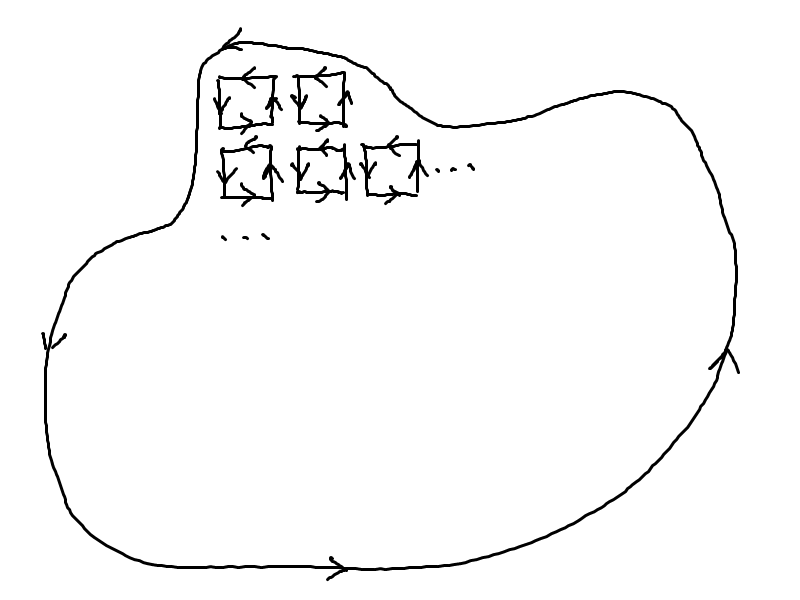
\includegraphics[width=0.33\linewidth]{fig/stokes-prove.png}
\caption{大家一起高速旋转}
\label{fig-stokes-prove}
\end{figure}

高斯定理和斯托克斯定理在二维情况下也成立,一维情况就是微积分中的牛顿-莱布尼兹定理:$F(b)-F(a)=\int_a^b F'(x) \opd x$。它们都把区域的边界和内部联系了起来。
\section{克罗内克张量$\delta_{i j}$;列维-奇维塔张量$\epsilon_{i j k}$;一些矢量公式}
方便起见,这一节用$1,2,3$表示$x,y,z$坐标,$\partial_i$表示$\frac{\partial}{\partial i}$。在三维直角坐标系中,$1 \le i,j \le 3$,$\mathbf{A}$就是$A_i$,$\nabla$就是$\partial_i$。

矢量$A_i$是有一个下标的量,张量则是有很多下标的量。矢量也是一种张量,前面的张量积$\nabla \mathbf{A}$则是有两个下标的张量。接下来我们用张量来表示一些矢量运算的公式,还会发现前面说的爱因斯坦求和约定非常方便。

(其实张量必须满足一些变换的规律,这里先不讲了。这里也不区分自由指标和哑指标)

矢量的点积$\mathbf{A} \cdot \mathbf{B}=\sum_{i=1}^3 A_i B_i$。按照爱因斯坦求和约定,下标相同就表示求和,求和号可以不写。也就是说,$\mathbf{A} \cdot \mathbf{B}=A_i B_i$。这样求和一次,式子中的下标就会减少两个,称为下标缩并。

克罗内克张量$\delta_{i j}=\begin{cases} 1, &i=j \\ 0, &i \neq j \end{cases}$。在三维情况下,$\delta_{i j}=\begin{bmatrix}
1 & 0 & 0 \\
0 & 1 & 0 \\
0 & 0 & 1
\end{bmatrix}$。如果把$\delta_{i j}$与$A_j$缩并,$\delta_{i j} A_j=A_i$,相当于给$A$换一个下标。

接下来讲一个复杂一些的张量:列维-奇维塔张量$\epsilon_{i j k}$,又叫排序张量。如果$ijk$分别是$123$,$231$或者$312$,那么$\epsilon_{i j k}=1$;如果$ijk$分别是$321$,$213$或者$132$,那么$\epsilon_{i j k}=-1$;否则$ijk$中至少有两个相同,$\epsilon_{i j k}=0$。它的分量形式这里就不写了,因为我懒。

矢量的叉积$\mathbf{A} \times \mathbf{B}=\epsilon_{i j k} A_j B_k$。它的左边是矢量,右边有一个自由指标$i$没有被求和,所以也是矢量。任何公式两边的自由指标必须是相同的(左边的矢量可以脑补下标$i$),而被求和的指标(哑指标,这里是$j,k$)可以不同。通过枚举可以发现:
\begin{align*}
(\mathbf{A} \times \mathbf{B})_1&=A_2 B_3-A_3 B_2 \\
(\mathbf{A} \times \mathbf{B})_2&=A_3 B_1-A_1 B_3 \\
(\mathbf{A} \times \mathbf{B})_3&=A_1 B_2-A_2 B_1
\end{align*}

容易发现,$\delta_{i j}=\delta_{j i}$,$\epsilon_{i j k}=\epsilon_{j k i}=-\epsilon_{j i k}$。还有一个公式:$\epsilon_{i j k} \epsilon_{k l m}=\delta_{i l} \delta_{j m}-\delta_{i m} \delta_{j l}$。这个公式也可以通过枚举来证明(虽然很麻烦):两边各有四个自由指标$i,j,l,m$,分别代进去$1,2,3$,共有81种情况,然后会发现它确实是对的。

接下来可以推导更复杂的公式:$(\mathbf{A} \times \mathbf{B}) \times \mathbf{C}=(\mathbf{A} \cdot \mathbf{C})\mathbf{B}-(\mathbf{B} \cdot \mathbf{C})\mathbf{A}$。
\begin{align*}
(\mathbf{A} \times \mathbf{B}) \times \mathbf{C}&=\epsilon_{i j k} (\epsilon_{j l m} A_l B_m) C_k \\
&=\epsilon_{i j k} \epsilon_{j l m} A_l B_m C_k
\internote{($\delta_{i j},\epsilon_{i j k},A_i$的指标缩并满足交换律和结合律)}
&=\epsilon_{k i j} \epsilon_{j l m} A_l B_m C_k \\
&=(\delta_{k l} \delta_{i m}-\delta_{k m} \delta_{i l}) A_l B_m C_k \\
&=\delta_{k l} \delta_{i m} A_l B_m C_k-\delta_{k m} \delta_{i l} A_l B_m C_k \\
&=A_k B_i C_k-A_i B_k C_k \\
&=(\mathbf{A} \cdot \mathbf{C})\mathbf{B}-(\mathbf{B} \cdot \mathbf{C})\mathbf{A}
\end{align*}

可以看出,如果在$(\mathbf{A} \times \mathbf{B}) \times \mathbf{C}$中交换$\mathbf{A}$和$\mathbf{B}$,结果会变成相反数。但是如果交换$\mathbf{A}$和$\mathbf{C}$,结果会完全不一样。

【练习】证明$\mathbf{A} \times (\mathbf{B} \times \mathbf{C})=(\mathbf{A} \cdot \mathbf{C})\mathbf{B}-(\mathbf{A} \cdot \mathbf{B})\mathbf{C}$。

把这个式子中的$\mathbf{A}$和$\mathbf{B}$换成$\nabla$,$\mathbf{C}$换成$\mathbf{A}$,还可以证明$\nabla \times (\nabla \times \mathbf{A})=\nabla(\nabla \cdot \mathbf{A})-(\nabla \cdot \nabla) \mathbf{A}$。

$(\nabla \cdot \nabla)$可以写成$\nabla^2$,称为拉普拉斯算符。在三维直角坐标系里,它就是$\ppxn{2}+\ppyn{2}+\ppzn{2}$。它没有下标,$\nabla^2 f$仍然是标量,$\nabla^2 \mathbf{A}$仍然是矢量。

但是要注意,$\partial_i$与$A_i$不满足交换律,因为$\partial_i$是对右边的东西求导,而$\partial_i$与$\partial_j,\delta_{i j},\epsilon_{i j k}$仍然满足交换律。比如要证明$\nabla \cdot (\mathbf{A} \times \mathbf{B})=\mathbf{B} \cdot (\nabla \times \mathbf{A})-\mathbf{A} \cdot (\nabla \times \mathbf{B})$:
\begin{align*}
\nabla \cdot (\mathbf{A} \times \mathbf{B})&=\partial_i (\epsilon_{i j k} A_j B_k) \\
&=\epsilon_{i j k} \partial_i(A_j B_k) \\
&=\epsilon_{i j k} (B_k \partial_i A_j+A_j \partial_i B_k) \\
&=B_k \epsilon_{k i j} \partial_i A_j+A_j \epsilon_{j k i} \partial_i B_k \\
&=B_k \epsilon_{k i j} \partial_i A_j-A_j \epsilon_{j i k} \partial_i B_k \\
&=\mathbf{B} \cdot (\nabla \times \mathbf{A})-\mathbf{A} \cdot (\nabla \times \mathbf{B})
\end{align*}

矢量分析当中常用的公式就是这么多,以后用到的时候可以翻回来看看。

\chapter{理论力学}
\section{广义坐标;拉格朗日量}
高中里我们学的是牛顿力学,但是世界上除了牛顿力学,还有别的力学体系,拉格朗日力学是其中常用的一种。要学习拉格朗日力学,首先要忘掉牛顿力学的世界观。假设我们不知道什么叫力,什么叫能量,什么叫速度,也不知道牛顿定律之类的东西。

我们要研究一个力学系统,就要用一些坐标来描述它。比如平面上的一个点可以用直角坐标$x$、$y$来描述,也可以用极坐标$r$、$\theta$来描述。如图\ref{fig-double-pend},平面内的双摆可以用坐标$\theta$、$\phi$来描述。
\begin{figure}[htb]
\centering
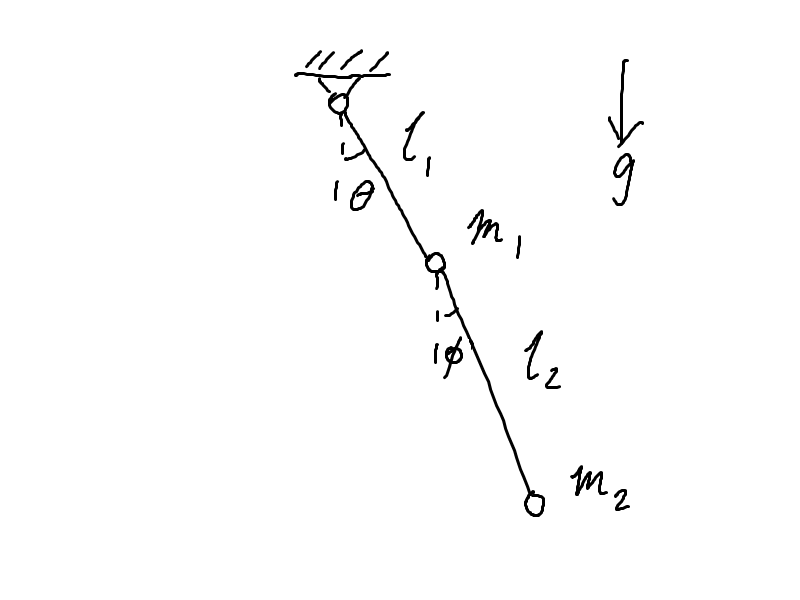
\includegraphics[width=0.33\linewidth]{fig/double-pend.png}
\caption{双摆}
\label{fig-double-pend}
\end{figure}

这里的坐标一般是位置或者角度,也可以是电量、温度等等。牛顿力学中的速度有时候也可以作为这里的坐标,但是现在先不考虑这件事情。

坐标对时间的导数叫作速度。出于习惯,用$\dot x$表示$\frac{\opd x}{\opd t}$,$\dot x^2$表示$(\frac{\opd x}{\opd t})^2$,而不是$\frac{\opd x^2}{\opd t}$,$\ddot x$表示$\frac{\opd^2 x}{\opd t^2}$。

拉格朗日力学的第一个基本假设是:每个力学系统都有一个“拉格朗日量”。比如一个小球在竖直平面内,用坐标$x$、$y$描述它的位置,考虑沿$-y$方向的重力场,那么它的拉格朗日量是
\begin{equation*}
L=\frac{1}{2}m(\dot x^2+\dot y^2)-m g y
\end{equation*}

诶这个东西看起来很像牛顿力学中的能量,但是仔细看会发现势能的正负号反了一下。拉格朗日量一般是坐标和速度的函数,而不会出现坐标的二阶或更高阶导数,而坐标和速度又是时间的函数。如果出现随时间变化的电场之类的环境条件,那么拉格朗日量本身还是时间的函数,但是现在也不考虑这件事情。

这个基本假设并不能告诉我们拉格朗日量是什么,就像从牛顿第二定律不能推出万有引力定律$F=\frac{G M m}{r^2}$一样。它们需要用其他方法推导出来,并且经过实验验证。比如自由粒子的拉格朗日量为$\frac{1}{2}m \mathbf{v}^2$,有质量的粒子在$-y$方向的重力场里要增加一项$-m g y$,带电粒子在电场中要增加一项$-q \phi$,在磁场中要增加一项$q \mathbf{v} \cdot \mathbf{A}$(这个看不懂可以先不管)。

图\ref{fig-double-pend}中双摆的拉格朗日量是
\begin{equation*}
L=\frac{1}{2}m_1 l_1^2 \dot \theta^2+\frac{1}{2}m_2 l_2^2 \dot \phi^2+m_1 g l_1 \cos \theta+m_2 g (l_1 \cos \theta+l_2 \cos \phi)
\end{equation*}

这已经是很复杂的拉格朗日量了,接下来要遇到的东西没有这么复杂。
\section{变分;拉格朗日方程}
把拉格朗日量写出来之后,可以用它来算出物体的运动情况。简单起见,假设系统只有一个坐标$q$,速度为$\dot q$。如果已知物体在时间$t_1$的坐标为$q_1$,时间$t_2$的坐标为$q_2$,但是不知道$t_1$和$t_2$之间的坐标$q(t)$。现在定义一个\emph{作用量}
\begin{equation*}
S=\int_{t_1}^{t_2} L(q(t),\dot q(t)) \opd t
\end{equation*}

它表示物体在$t_1$和$t_2$之间的运动。物体可以做我们熟悉的斜抛之类的运动,也可以做各种奇怪的运动,如图\ref{fig-strange-move},只要保证$q(t_1)=q_1$,$q(t_2)=q_2$这两个边界条件就行。
\begin{figure}[htb]
\centering
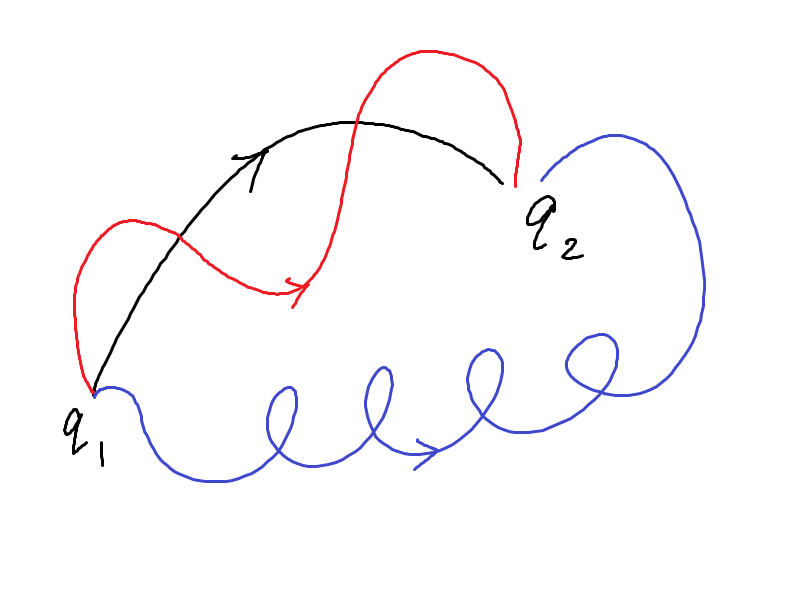
\includegraphics[width=0.33\linewidth]{fig/strange-move.png}
\caption{奇怪的运动}
\label{fig-strange-move}
\end{figure}

现在是拉格朗日力学的第二个基本假设:在这些奇怪的运动当中,真正的运动算出来的$S$是一个极小值。用数学语言来描述,就是
\begin{equation*}
\opvar S=0
\end{equation*}

这就是传说中的\emph{变分原理}!!是不是觉得拉格朗日的脑洞比牛顿还大?

(前方高能,看不懂可以先跳过)

$\opvar$表示变分,它的作用和求导差不多,而且目前我们认为它和积分、求导可以交换顺序。
\begin{align*}
\opvar S&=\opvar \int_{t_1}^{t_2} L(q(t),\dot q(t)) \opd t \\
&=\int_{t_1}^{t_2} \opvar L(q(t),\dot q(t)) \opd t \\
&=\int_{t_1}^{t_2}(\frac{\partial L}{\partial q} \opvar q+\frac{\partial L}{\partial \dot q} \opvar \dot q)\opd t \\
&=\int_{t_1}^{t_2}\frac{\partial L}{\partial q} \opvar q \opd t+\int_{t_1}^{t_2}\frac{\partial L}{\partial \dot q} (\opvar \frac{\opd q}{\opd t}) \opd t \\
&=\int_{t_1}^{t_2}\frac{\partial L}{\partial q} \opvar q \opd t+\int_{t_1}^{t_2}\frac{\partial L}{\partial \dot q} (\opdt \opvar q) \opd t
\end{align*}

对后面一项用分部积分:
\begin{align*}
\opdt(\frac{\partial L}{\partial \dot q} \opvar q)&=\opdt(\frac{\partial L}{\partial \dot q}) \opvar q+\frac{\partial L}{\partial \dot q} (\opdt \opvar q) \\
\frac{\partial L}{\partial \dot q} (\opdt \opvar q)&=\opdt(\frac{\partial L}{\partial \dot q} \opvar q)-\opdt(\frac{\partial L}{\partial \dot q}) \opvar q \\
\int_{t_1}^{t_2}\frac{\partial L}{\partial \dot q} (\opdt \opvar q) \opd t&=\int_{t_1}^{t_2} \opdt(\frac{\partial L}{\partial \dot q} \opvar q) \opd t-\int_{t_1}^{t_2}\opdt(\frac{\partial L}{\partial \dot q}) \opvar q \opd t\\
&=\left. \frac{\partial L}{\partial \dot q} \opvar q \right|_{t_1}^{t_2}-\int_{t_1}^{t_2}\opdt(\frac{\partial L}{\partial \dot q}) \opvar q \opd t
\end{align*}

$t_1$和$t_2$时的坐标是确定的,所以$\opvar q=0$,只剩下后面一项。继续算$\opvar S$:
\begin{align*}
\opvar S&=\int_{t_1}^{t_2}\frac{\partial L}{\partial q} \opvar q \opd t-\int_{t_1}^{t_2}\opdt(\frac{\partial L}{\partial \dot q}) \opvar q \opd t \\
&=\int_{t_1}^{t_2}(\frac{\partial L}{\partial q}-\opdt\frac{\partial L}{\partial \dot q}) \opvar q \opd t
\end{align*}

(高能部分结束)

要让$\opvar S=0$,那么$\frac{\partial L}{\partial q}-\opdt \frac{\partial L}{\partial \dot q}=0$。这就是拉格朗日力学中的运动方程。

有多个坐标的时候的推导也是类似的。比如有两个坐标$x$和$y$,那么就有两个方程$\frac{\partial L}{\partial x}-\opdt \frac{\partial L}{\partial \dot x}=0$,$\frac{\partial L}{\partial y}-\opdt \frac{\partial L}{\partial \dot y}=0$。

用掉下来的小球的例子试一试:$L=\frac{1}{2}m(\dot x^2+\dot y^2)-m g y$,$\frac{\partial L}{\partial y}=-m g$,$\frac{\partial L}{\partial \dot y}=m \dot y$,$\opdt \frac{\partial L}{\partial \dot y}=m \ddot y$,代入运动方程得到$-m g-m \ddot y=0$,也就是说$\ddot y=-g$,跟我们的常识一样。

(注意:对$q$求导时$\dot q$当作常数,对$\dot q$求导时$q$当作常数)

严格来说,变分为零只表示作用量达到极值或者稳定值,而不一定是极小值,跟导数的道理一样。但是物理问题里遇到的一般都是极小值,所以“作用量取极小值”成了一个约定俗成的说法。

在力学范围内,拉格朗日量是坐标和速度的函数,所以只要知道系统在某个时刻的坐标和速度,就能算出它在从前和将来任何时候的坐标、速度、加速度、能量等情况,这就是牛顿时代决定论的思想。但是热学范围内出现了一些不能这样描述,或者说不可逆的过程,比如粘滞阻力或者铁的磁化,怎样用力学原理来解释这些现象是至今还在研究的问题。

变分原理在物理学的其他领域也会出现,比如光学里的光程最短原理,只要定义作用量为$S=\int_{\mathbf{r}_1}^{\mathbf{r}_2} n(\mathbf{r}) \opd \mathbf{r}$,$\mathbf{r}$表示空间中的位置,$n(\mathbf{r})$表示这个位置的折射率,那么$\opvar S=0$就能给出光走的路线。
\section{对称性与守恒量;动量;能量}
还是看掉下来的小球的例子:$L=\frac{1}{2}m(\dot x^2+\dot y^2)-m g y$。如果对$x$坐标列运动方程会怎么样呢?拉格朗日量不含$x$,所以$\frac{\partial L}{\partial x}=0$,$x$坐标的运动方程就是$\ddot x=0$。

现在定义$\frac{\partial L}{\partial \dot q}$叫作坐标$q$对应的动量$p_q$。在上面的例子中,$x$坐标对应的动量就是$m \dot x$,跟牛顿力学一样。因为拉格朗日量不含$x$,所以$\opdt p_x=0$,这个动量是守恒的。

拉格朗日量不含$x$,也可以说系统具有空间平移对称性。所以就有了这样一句话:空间的平移对称性导致动量守恒。

刚才的数学推导看起来很厉害,现在用人话再解释一遍。如果一个小球在一片平地上跑,它向前跑了一段,前面还是一片平地,也就是说系统平移之后和原来一样,因此我们说系统具有平移对称性。在这样的系统中,小球没有理由改变它的动量,动量是守恒的。

(系统平移之后,小球的位置(或者说坐标)就变了,但是拉格朗日量的表达式不变,所以我们认为系统和原来一样。关于对称性的严格定义以后应该会单独讲)

如果小球向前跑,撞到一面墙弹回来,它的动量就不守恒了。这个系统没有平移对称性,如果把系统平移一下,墙的位置就变了。也就是说,平移对称性的破缺导致动量守恒的破缺。如果小球在斜坡上跑,它会越跑越快。虽然向前跑一段之后,斜坡的斜率还是和原来一样,但是高度变了(或者说重力势能与水平坐标的关系变了),所以这个系统没有平移对称性,动量也就不守恒。

如果拉格朗日量不含时间$t$,又会发生什么呢?
\begin{align*}
\opdt L&=\frac{\partial L}{\partial q} \frac{\opd q}{\opd t}+\frac{\partial L}{\partial \dot q} \frac{\opd \dot q}{\opd t} \\
&=(\opdt \frac{\partial L}{\partial \dot q}) \frac{\opd q}{\opd t}+\frac{\partial L}{\partial \dot q} \frac{\opd \dot q}{\opd t} \\
&=\opdt(\frac{\partial L}{\partial \dot q} \dot q) \\
&=\opdt(p \dot q)
\end{align*}

(注意:因为拉格朗日量不含$t$,所以不会出现$\frac{\partial L}{\partial t}$)

移项得到$\opdt(p \dot q-L)=0$,所以可以定义$p \dot q-L$叫作能量$E$。如果有多个坐标,那么能量$E=\sum_i p_i \dot q_i-L$。用掉下来的小球算一下会发现这个能量和牛顿力学里的能量其实是一样的。

也就是说,时间的平移对称性导致能量守恒。比如一个单摆挂在那里摆动,过了一段时间,系统还是和原来一样,所以单摆的能量是守恒的。如果过了一段时间,突然让单摆带电,并且在空间中加一个电场,这个系统就没有时间平移对称性,能量也就不守恒了。这里没有考虑摩擦力、空气阻力之类的,事实上这些力在拉格朗日力学当中不能用简单的方法处理,但是我们认为它们会破坏系统的时间平移对称性。

如果坐标是角度,那么对应的动量就是牛顿力学中的角动量。但是拉格朗日力学对角动量有另外的定义,空间的旋转对称性导致角动量守恒,这里先不讲了。对称与守恒在物理学当中非常重要,以后我们还会遇到更奇怪的对称性和它对应的守恒量。

总而言之,拉格朗日力学是一种与牛顿的基础完全不同的力学方法,它的优点在于不用做受力分析,而且容易处理守恒量。工程师用电脑计算桥梁之类的复杂结构用的就是这种方法,因为电脑很难做受力分析,但是适合算各种偏导数。现代的粒子物理当中,两个粒子之间“力”的概念也很难说清楚,所以也要用这种方法处理。如果我们发现了新的粒子,想办法确定它的拉格朗日量是一件很重要的事情。
\section{虚功原理}
拉格朗日力学只是扩大一下大家的眼界,现在我们回到牛顿力学。

一个掉下来的小球,它的能量是$E=\frac{1}{2}m(\dot x^2+\dot y^2)+m g y$。把能量对时间求导:
\begin{align*}
\opdt E&=m(\dot x \ddot x+\dot y \ddot y)+m g \dot y \\
&=m \ddot x \dot x+(m \ddot y+m g) \dot y
\end{align*}

又因为能量守恒,$\opdt E=0$。不管小球的速度是多少,这个式子都是成立的,而且$\dot x$和$\dot y$是无关的,所以它们前面的系数都要为$0$,于是我们得到了$\ddot x=0$,$\ddot y=-g$。

(这样推导应该比拉格朗日量之类的好理解一点,但是如果承认拉格朗日量就是动能减势能,通过一些分部积分,这种方法和拉格朗日力学的基本假设是可以互相推导的。为什么说$\dot x$和$\dot y$是无关的呢?这个待会再讲)

很多书都在静力学中用虚功原理,事实上在动力学中也是可以用的。
\begin{figure}[htb]
\centering
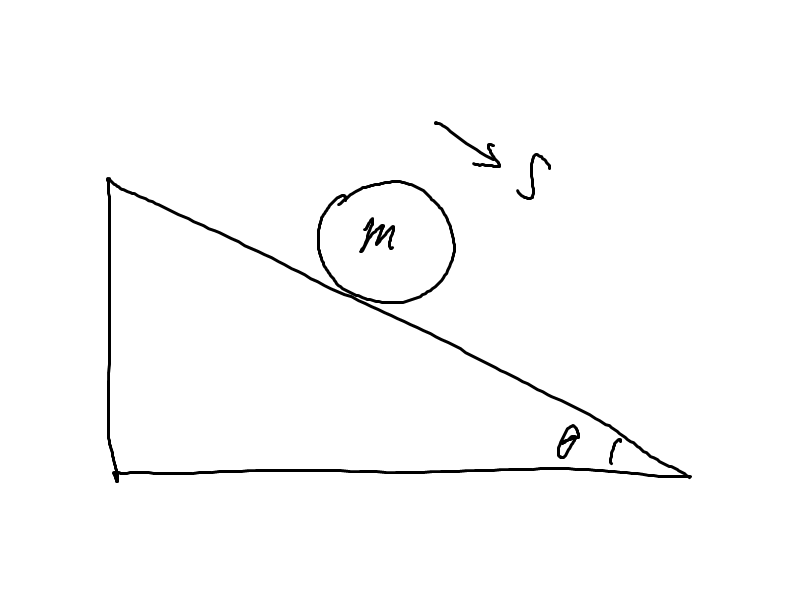
\includegraphics[width=0.33\linewidth]{fig/slope-ball.png}
\caption{卧槽,一个球滚下来了!}
\label{fig-slope-ball}
\end{figure}

现在来看一个复杂一点的例子:如图\ref{fig-slope-ball},一个固定粗糙斜面倾角为$\theta$,一个质量为$m$的均匀空心球壳无滑动地滚下来,设沿斜面的位移为$s$,球心的速度就是$\dot s$,但是考虑转动之后,它的动能不是$\frac{1}{2} m \dot s^2$,而是$\frac{5}{6} m \dot s^2$,现在要算它滚下来的加速度。正常的自招书上会用受力分析啊转动定律啊速度关联之类的来算,但是现在我们用虚功原理。

先写出系统的能量:$E=\frac{5}{6} m \dot s^2+m g s \sin \theta$,然后对时间求导:$(\frac{5}{3} m \ddot s+m g \sin \theta) \dot s=0$,所以$\ddot s=-\frac{3}{5} g \sin \theta$。

【练习】如果是均匀实心球,那么动能是$\frac{7}{10} m \dot s^2$。求它的加速度,然后算出速度和位移关于$t$的函数,并且验证能量确实是守恒的。
\section{约束;自由度}
再增加一点难度:假设斜面是会动的,质量为$M$。但是斜面是光滑的,这样球就不会转动,它的动能是$\frac{1}{2} m v^2$,否则太难了。
\begin{figure}[htb]
\centering
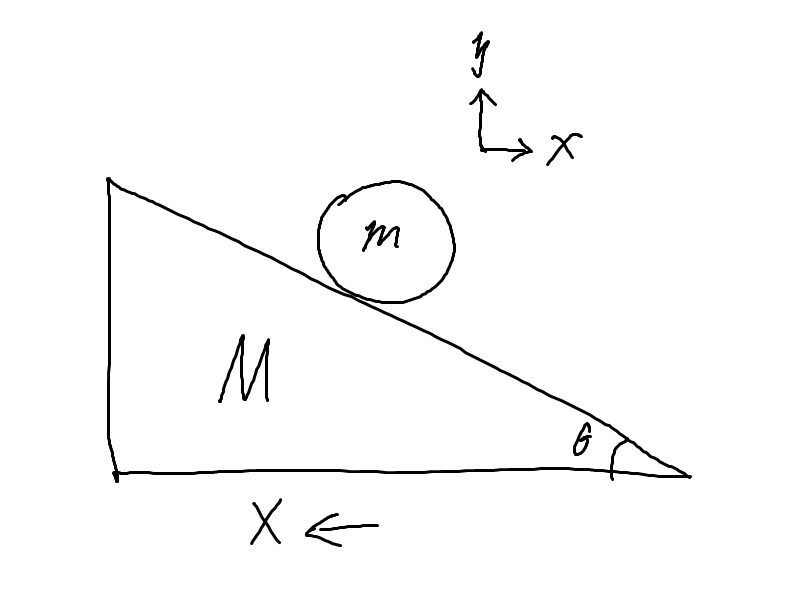
\includegraphics[width=0.33\linewidth]{fig/slope-ball-2.png}
\caption{卧槽,球和斜面都在动!}
\label{fig-slope-ball-2}
\end{figure}

现在把坐标设为$s$就不太方便了,如图\ref{fig-slope-ball-2},把$M$向左的位移设为$X$,把$m$的位移设为$x$和$y$。系统的能量是$E=\frac{1}{2} M \dot X^2+\frac{1}{2} m (\dot x^2+\dot y^2)+m g y$。

但是!坐标$X$、$x$和$y$并不是无关的。小球必须在斜面上,所以有一个约束条件$y=-(X+x) \tan \theta$。这个约束条件还可以求导得到$\dot y=-(\dot X+\dot x) \tan \theta$。

在$E$里把$y$消掉,得到$E=\frac{1}{2} M \dot X^2+\frac{1}{2} m (\dot x^2+(\dot X+\dot x)^2 \tan^2 \theta)-m g (X+x) \tan \theta$。

现在$X$和$x$是无关的,把能量对时间求导,经过各种化简得到$((M+m \tan^2 \theta) \ddot X+m \tan^2 \theta \ddot x-m g \tan \theta)\dot X+(m \tan^2 \theta \ddot X+m (1+\tan^2 \theta) \ddot x-m g \tan \theta)\dot x=0$。

要求$\dot X$和$\dot x$的系数都为零,解得$\ddot X=\frac{m \tan \theta}{M (1+\tan^2 \theta)+m \tan^2 \theta} g$,$\ddot x=\frac{M \tan \theta}{M (1+\tan^2 \theta)+m \tan^2 \theta} g$。代入$y$的式子得$\ddot y=-\frac{(M+m) \tan^2 \theta}{M (1+\tan^2 \theta)+m \tan^2 \theta} g$。

把题目做完之后,考虑几个特殊情况:如果$M \gg m$,那么跟斜面不动的时候一样,$\ddot y=-g \tan^2 \theta$;如果$M \ll m$,那么小球几乎是竖直掉下来,$\ddot y=-g$。

这个系统有$3$个坐标,$1$个约束,所以有$3-1=2$个独立的坐标,或者说有$2$个自由度。如果把斜面左右移动设为一个坐标,小球沿着斜面上下移动设为另一个坐标,那么就没有约束条件了,系统仍然有$2$个自由度。同一个系统,不管选择什么坐标,自由度的数量总是一样的。

比如三维空间中的质点有$3$个自由度,不管你用直角坐标、柱坐标还是球坐标。如果是一个会转的小球,要确定它的方向,就多了$3$个转动自由度,总共$6$个自由度。

(严格来说这里只考虑完整约束,也就是斜面与小球的位置关系,而与它们的速度无关。非完整约束这里先不讲)

我们发现$M \dot X=m \dot x$(注意$X$和$x$设的正方向),也就是水平方向动量守恒。动量守恒并不是一个约束条件,而且一般情况下能量守恒和动量守恒是不能互推的。但是如果把动量守恒当作一个已知条件,上面的计算可以简化一些。

【练习】把约束条件和动量守恒代到能量的式子里,这样就只剩下一个坐标了,然后算出各个加速度。
\section{拉格朗日乘子法}
有两个函数$f(x_1,x_2,\dots,x_n)$和$g(x_1,x_2,\dots,x_n)$,在$g=0$的条件下,求$f$的极值。

设$L=f+\lambda g$,$\lambda$是一个待定常数。解这样的方程组:
\begin{equation*}
\begin{cases}
\frac{\partial L}{\partial x_1}=0 \\
\frac{\partial L}{\partial x_2}=0 \\
\dots \\
\frac{\partial L}{\partial x_n}=0 \\
g=0
\end{cases}
\end{equation*}

共有$n+1$个方程,$n+1$个未知数($n$个$x$和一个$\lambda$),可以把各个$x$解出来,这些$x$代入$f$有可能取到极值。(但是也有可能不是极值,这只是一个必要条件,算出来的$x$需要检验)

举个栗子:$f=x+y$,$g=x^2+y^2-1$,很容易看出来$f_\text{max}=f(\frac{\sqrt{2}}{2},\frac{\sqrt{2}}{2})=\sqrt{2}$,$f_\text{min}=f(-\frac{\sqrt{2}}{2},-\frac{\sqrt{2}}{2})=-\sqrt{2}$。现在用这种方法来试一试。
\begin{gather*}
L=x+y+\lambda x^2+\lambda y^2-\lambda \\
\begin{cases}
\frac{\partial L}{\partial x}=1+2 \lambda x=0 \\
\frac{\partial L}{\partial y}=1+2 \lambda y=0 \\
x^2+y^2-1=0
\end{cases} \\
x=-\frac{1}{2 \lambda},y=-\frac{1}{2 \lambda} \\
\frac{1}{4 \lambda^2}+\frac{1}{4 \lambda^2}-1=0 \\
\lambda=\pm \frac{\sqrt{2}}{2} \\
\begin{cases}
x=\frac{\sqrt{2}}{2} \\
y=\frac{\sqrt{2}}{2}
\end{cases}\text{或{}}\begin{cases}
x=-\frac{\sqrt{2}}{2} \\
y=-\frac{\sqrt{2}}{2}
\end{cases}
\end{gather*}

这种方法的原理是什么呢?在上面的例子中,考虑矢量$\nabla g=(\frac{\partial g}{\partial x},\frac{\partial g}{\partial y})=(2x,2y)$,它是坐标的函数,可以认为平面上的每个点$(x_0,y_0)$上都放着一个矢量$(2x_0,2y_0)$,所以说$\nabla g$是一个矢量场。(觉得$\nabla g$这个符号奇怪吗?以后会习惯的)

$g=0$是平面上的一个圆,当点$(x_0,y_0)$在圆上时,$\nabla g$垂直于圆在这个点的切线。一般的约束条件$g(x,y)=0$表示二维平面上的一条曲线,$\nabla g$垂直于这条曲线的切线。

再考虑矢量场$\nabla f=(\frac{\partial f}{\partial x},\frac{\partial f}{\partial y})$,它的方向是$f$变化最快的方向。如果$\nabla f+\lambda \nabla g=0$,那么$\nabla f$与$\nabla g$平行,也就是说$f$变化最快的方向与曲线$g=0$的切线垂直,$f$有可能在这里取到极值。

【练习】已知$x^2+y^2+z^2=1$,求$2x y+y z+z x$的最大值。

如果$f$和$g$都是一到二次多项式,但是配方一下子配不出来,这种方法说不定可以救你一命。如果$f$和$g$的形式比较复杂,有分式或者根号,这种方法就需要比较大的计算量。

如果有多个约束条件$g_1=0,g_2=0,\dots,g_n=0$,那么就要设$L=f+\sum_{i=1}^n \lambda_i g_i$,然后用上面的方程组把各个$x$和各个$\lambda$解出来。

这是一个数学问题,但是拉格朗日给了它一个物理意义:假设一个小球串在细铁丝做的形状为曲线$g=0$的环上,然后放在势能为$f$的场里,小球会跑到势能极低的位置。环给小球的支持力的方向垂直于环的切线,大小就是$\lambda$。

\chapter{电动力学}
\rightline{\it 电动力学是电的动力学,而不是电动的力学。}
\section{麦克斯韦方程组}
我们先来看看传说中的麦克斯韦方程组:
\begin{align*}
\nabla \cdot \mathbf{E}&=\frac{\rho}{\epsilon_0} & \nabla \cdot \mathbf{B}&=0 \\
\nabla \times \mathbf{E}&=-\frac{\partial \mathbf{B}}{\partial t} & \nabla \times \mathbf{B}&=\mu_0 \mathbf{j}+\frac{1}{c^2} \frac{\partial \mathbf{E}}{\partial t}
\end{align*}

这是麦克斯韦方程组在真空中的形式,没有考虑电磁介质。这些方程可以解出所有与电和磁有关的现象(如果不考虑量子效应),包括高中学过的库仑定律、楞茨定律等等,也包括电磁介质的性质。如果你第一次看到这些方程的时候一脸懵逼,连里面的三角形是什么意思都不知道,那也不用害怕,这一章我们会慢慢搞懂这些方程的意思。
\section{前两个麦克斯韦方程}
高中学过了点电荷周围的电场$E=k \frac{q}{r^2}$,如果以电荷为中心画一个半径为$r$的球面,$\mathbf{E}$的通量$\Phi=E \cdot 4 \pi r^2=4 \pi k q$。因为电场线是连续的,不管在外面画什么样的闭合曲面,上面的$\Phi$都是$4 \pi k q$。

如图\ref{fig-elec-flux},如果有许多电荷,曲面上的$\Phi$是曲面内各个电荷产生的$\Phi$之和;而曲面外的电荷产生的电场线在进入曲面之后肯定要出来,对$\Phi$没有影响。
\begin{figure}[htb]
\centering
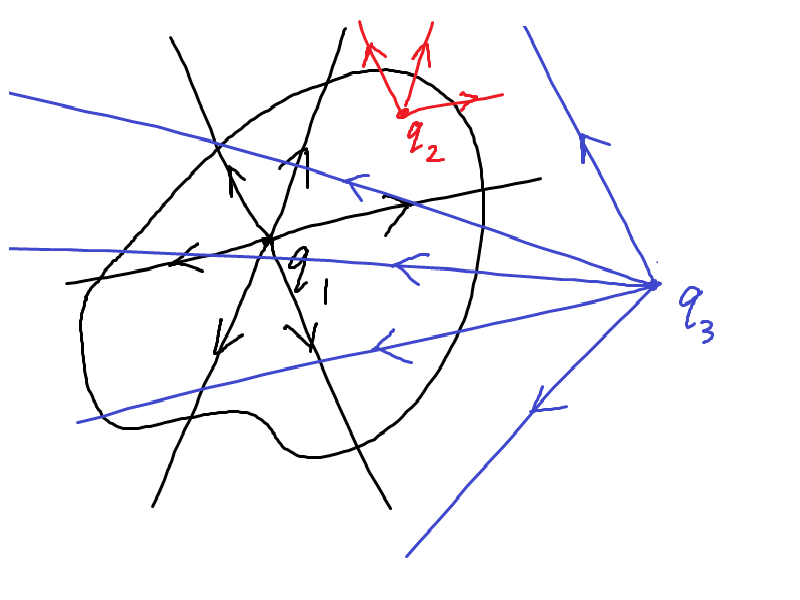
\includegraphics[scale=0.5]{fig/elec-flux.png}
\caption{里面和外面}
\label{fig-elec-flux}
\end{figure}

(这里分别画出了各个电荷产生的电场线,不用考虑它们的相互影响。电场线在某个点的方向就是这个点上$\mathbf{E}$的方向,我们经常看到两个电荷之间用弯曲的电场线连接,那是每个电荷产生的$\mathbf{E}$的矢量和。如果电场线从一个电荷开始,从另一个电荷终止,相当于这两个电荷的一条电场线相互抵消)

也就是说,$\Phi=4 \pi k \sum_V q_i$。在电动力学中会用另一个常量$\epsilon_0=\frac{1}{4 \pi k}$,称为真空介电常量,$\epsilon_0 \approx 8.85 \times 10^{-12} \unit{m^{-3} \cdot kg^{-1} \cdot s^4 \cdot A^2}$。如果把公式里的$k$换成$\epsilon_0$,就是$\Phi=\frac{1}{\epsilon_0} \sum_V q_i$。用$\epsilon_0$可以少写很多$4 \pi$。

按照高斯定理,$\Phi=\int_V \nabla \cdot \mathbf{E} \opd V$。这里有对$V$的积分,如果要把前面对$V$的求和改成积分,就要把电荷$q$改成电荷密度$\rho$:$\Phi=\frac{1}{\epsilon_0} \int_V \rho \opd V$。比较两个式子,可以发现$\nabla \cdot \mathbf{E}=\frac{\rho}{\epsilon_0}$。也就是说,第一个麦克斯韦方程对应着库仑定律或者电场的高斯定理。

(以后学了量纲分析之后,你可以检验一下它两边的量纲一样,注意$\nabla$的量纲是$[L]^{-1}$)

现在第二个麦克斯韦方程应该很好理解:$\nabla \cdot \mathbf{B}=0$表示磁感线是闭合的,不会变多变少,除非存在传说中的磁单极子。
\section{后两个麦克斯韦方程}
第三个麦克斯韦方程$\nabla \times \mathbf{E}=-\frac{\partial \mathbf{B}}{\partial t}$对应着法拉第电磁感应定律。按照斯托克斯定理,$\oint_L \mathbf{E} \cdot \opd \mathbf{L}=\int_S (\nabla \times \mathbf{E}) \cdot \opd \mathbf{S}$。而法拉第定律可以写成$\oint_L \mathbf{E} \cdot \opd \mathbf{L}=-\int_S \frac{\partial \mathbf{B}}{\partial t} \cdot \opd \mathbf{S}$,左边表示$L$上的感生电动势,右边表示$S$上磁通量的变化速率,负号表示感生电动势的方向按照楞茨定律确定。

第四个麦克斯韦方程的右边有两项。如果只有$\nabla \times \mathbf{B}=\mu_0 \mathbf{j}$,它表示电流在周围产生磁场。$\mathbf{j}$是电流密度,也就是单位面积上流过的电流,为了把面积上的求和改成积分,就要把$I$改成$\mathbf{j}$。$I$是标量,然而$\mathbf{j}$是矢量,$I$是$\mathbf{j}$的通量。你可以检验一下磁场方向与电流方向的关系确实是右手螺旋。

$\mu_0$是一个比例系数,叫作真空磁导率,$\mu_0=4 \pi \times 10^{-7} \unit{m \cdot kg \cdot s^{-2} \cdot A^{-2}}$。

第二项$\frac{1}{c^2} \frac{\partial \mathbf{E}}{\partial t}$又是什么意思呢?如图\ref{fig-disp-curr},有两根很粗的导线靠近但不接触,中间形成一个平行板电容器,两个极板分别是两根导线的末端。如果导线内没有电流,但是导线的末端积累着电荷,中间就有恒定的电场;如果导线内有电流,中间的电场就会变化。
\begin{figure}[htb]
\centering
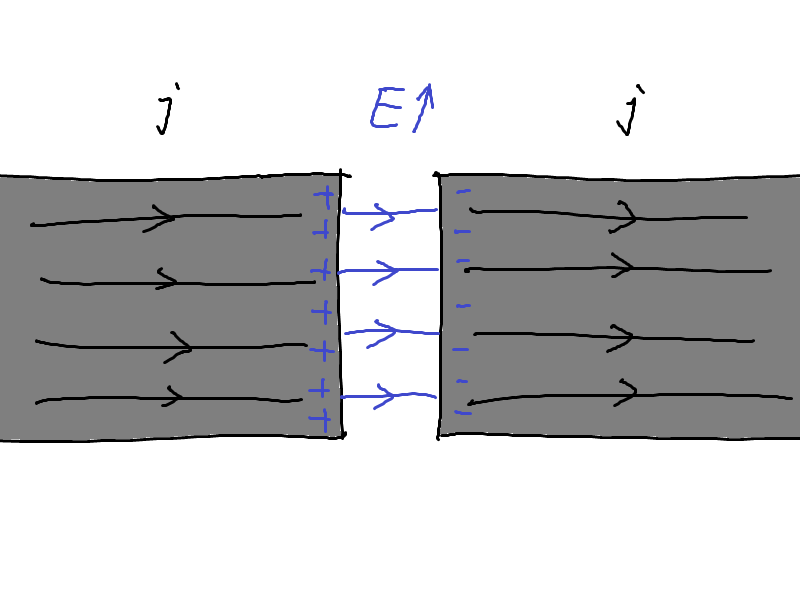
\includegraphics[scale=0.5]{fig/disp-curr.png}
\caption{位移电流}
\label{fig-disp-curr}
\end{figure}

电流会在周围产生磁场,所以麦克斯韦猜:变化的电场也会在周围产生磁场。所以他把变化变化的电流称为位移电流。准确地说,位移电流密度$\mathbf{j}_d=\epsilon_0 \frac{\partial \mathbf{E}}{\partial t}$,它的量纲与$\mathbf{j}$相同。

所以第四个麦克斯韦方程也可以写成$\nabla \times \mathbf{B}=\mu_0 (\mathbf{j}+\mathbf{j}_d)=\mu_0 \mathbf{j}+\epsilon_0 \mu_0 \frac{\partial \mathbf{E}}{\partial t}$。

我们可以定义另一个常数$c$,令$\epsilon_0 \mu_0=\frac{1}{c^2}$。$c$的量纲是速度,待会可以证明它是电磁波的速度。当时的人们用实验测出$\epsilon_0$和$\mu_0$,算出$c$,与其他方法测出的光速相同,所以麦克斯韦猜想光是一种电磁波。

$\frac{\partial \mathbf{E}}{\partial t}$前面的系数$\frac{1}{c^2}$非常小,所以从前一直没有被人们发现,直到麦克斯韦猜了出来,后来也得到了实验的证实。
\section{电磁波}
接下来我们用麦克斯韦方程组来算一些有意思的东西。既然变化的磁场在附近产生电场,变化的电场在附近产生磁场,那么它们可以不断产生并且向远处传播,即使在没有电荷和电流的\emph{自由空间}里也是一样。

在没有电流的情况下,$\nabla \times \mathbf{B}=\frac{1}{c^2} \frac{\partial \mathbf{E}}{\partial t}$。想办法让其他方程出现$\nabla \times \mathbf{B}$,可以对$\nabla \times \mathbf{E}=-\frac{\partial \mathbf{B}}{\partial t}$两边同时取旋度,得到$\nabla \times (\nabla \times \mathbf{E})=-\ppt(\nabla \times \mathbf{B})=-\frac{1}{c^2} \pptn{2} \mathbf{E}$。($\nabla \times$和$\ppt$可以交换顺序)

接着处理式子的左边,按照矢量分析的公式,$\nabla \times (\nabla \times \mathbf{E})=\nabla(\nabla \cdot \mathbf{E})-\nabla^2 \mathbf{E}$。在没有电荷的情况下,$\nabla \cdot \mathbf{E}=0$,剩下$-\nabla^2 \mathbf{E}$。

也就是说,$-\nabla^2 \mathbf{E}=-\frac{1}{c^2} \pptn{2} \mathbf{E}$,一般写成$\pptn{2} \mathbf{E}=c^2 \nabla^2 \mathbf{E}$,也就是$\pptn{2} \mathbf{E}=c^2 (\ppxn{2} \mathbf{E}+\ppyn{2} \mathbf{E}+\ppzn{2} \mathbf{E})$。简单起见,在一维情况下,$\pptn{2} \mathbf{E}=c^2 \ppxn{2} \mathbf{E}$,$\mathbf{E}$是$x,t$的函数。

如果把$\mathbf{E}$的某个分量记为$f$,它满足方程$\pptn{2} f=c^2 \ppxn{2} f$。只要解出这个标量方程,可以用相同的方法解矢量方程。

这就是传说中的\emph{波动方程},它是一个线性常系数齐次二阶偏微分方程。正常的电动力学课本会用分离变量之类的方法解这个方程,但是我们仍然只要猜:$f$可以是任何函数$f(x-c t)$,只要它只有一个自变量,而且就是$x-c t$。

$\ppt f=\frac{\partial f}{\partial(x-c t)}\frac{\partial(x-c t)}{\partial t}=-c \frac{\partial f}{\partial(x-c t)}$。同样,$\pptn{2} f=c^2 \frac{\partial^2 f}{\partial(x-c t)^2}$,$\ppxn{2} f=\frac{\partial^2 f}{\partial(x-c t)^2}$,所以$f$满足波动方程。

波动方程中只有$c$的二次项,如果把$c$换成$-c$,方程还是原来的方程,所以$f(x+c t)$也是方程的解。事实上,方程的通解是$f=f_1(x-c t)+f_2(x+c t)$,$f_1,f_2$可以是任何函数。

$f_1(x-c t)$表示沿$+x$方向传播的波,它的速度为$c$,形状可以是任意的,比如一个峰,而不一定是正弦波,而且在传播过程中不会改变形状。$f_2(x+c t)$则表示沿$-x$方向传播的波。

但是我们一般会研究(用复指数表示的)简谐波$f=C_1 \rme^{\rmi (k x-\omega t)}+C_2 \rme^{\rmi (k x+\omega t)}$,其中$k=\frac{\omega}{c}$。这样的波称为单色波,因为光的颜色是由频率决定的。以后学了傅立叶变换就会知道,即使$f$与时间的关系不是简谐振动,也可以分解成简谐振动的叠加。

电磁波里面有$\mathbf{E}$也有$\mathbf{B}$,现在解出了$\mathbf{E}$,然后利用$\nabla \times \mathbf{E}=-\frac{\partial \mathbf{B}}{\partial t}$可以算出$\mathbf{B}$。
\section{三维空间中的单色波}
虽然猜了这么多解,但是用正经的方法解偏微分方程还是要讲一下的。。

现在来看三维空间中的电磁波。仍然把$\mathbf{E}$或者$\mathbf{B}$的某个分量记为$f$,它满足波动方程
\begin{equation*}
\pptn{2} f=c^2 (\ppxn{2} f+\ppyn{2} f+\ppzn{2} f)
\end{equation*}

$f$是$x,y,z,t$的函数,上面的方程是偏微分方程,如果能把$x,y,z,t$分开,解起来就比较简单。

先把$t$与其他变量分开,仍然设$f$与时间的关系是简谐振动:$f=f_0(x,y,z) \rme^{-\rmi \omega t}$。

($f$与位置的关系也可以这样分解,比如$f=f_0(y,z,t) \rme^{\rmi k_x x}$。但是不能把位置和时间同时分解,因为接下来会看到,$k_x$与$\omega$是有关的。这里我们先固定$\omega$,然后求$f_0(x,y,z)$与$\omega$的关系)

这样一来,$\pptn{2} f=-\omega^2 f$。仍然令$k=\frac{\omega}{c}$,那么$\ppxn{2} f+\ppyn{2} f+\ppzn{2} f+k^2 f=0$。

再把$x,y,z$分开:令$f=X(x) Y(y) Z(z) \rme^{-\rmi \omega t}$,$X,Y,Z$都是只有一个自变量的函数。这样一来,$\ppxn{2} f=\frac{\partial^2 X(x)}{\partial x^2}  Y(y) Z(z) \rme^{-\rmi \omega t}=\frac{f}{X} \ppxn{2} X$。同样,$\ppy f=\frac{f}{Y} \ppyn{2} Y$,$\ppz f=\frac{f}{Z} \ppzn{2} Z$。

把它们代入波动方程,就得到了
\begin{align*}
\frac{f}{X} \ppxn{2} X+\frac{f}{Y} \ppyn{2} Y+\frac{f}{Z} \ppzn{2} Z+k^2 f&=0 \\
\frac{1}{X} \ppxn{2} X+\frac{1}{Y} \ppyn{2} Y+\frac{1}{Z} \ppzn{2} Z+k^2&=0
\end{align*}

再定义三个待定系数$k_x,k_y,k_z$,要求$k_x^2+k_y^2+k_z^2=k^2$,上面的式子可以分成三个常微分方程:
\begin{align*}
\frac{1}{X} \ppxn{2} X+k_x^2&=0 \\
\frac{1}{Y} \ppyn{2} Y+k_y^2&=0 \\
\frac{1}{Z} \ppzn{2} Z+k_z^2&=0
\end{align*}

这就是偏微分方程的分离变量,把关于多个自变量的偏微分方程变成关于各个自变量的常微分方程,然后分别解它们。

这三个方程都是我们熟悉的简谐振动方程,比如$\ppxn{2} X+k_x^2 X=0$,解得$X=C_1 \rme^{\rmi k_x x}+C_2 \rme^{-\rmi k_x x}$。最后$f$的解是($f$里面还有$\rme^{-\rmi \omega t}$,所以现在不用把指数形式改成三角形式)
\begin{equation*}
f=(C_1 \rme^{\rmi k_x x}+C_2 \rme^{-\rmi k_x x})(C_3 \rme^{\rmi k_y y}+C_4 \rme^{-\rmi k_y y})(C_5 \rme^{\rmi k_z z}+C_6 \rme^{-\rmi k_z z}) \rme^{-\rmi \omega t}
\end{equation*}

$k_x,k_y,k_z$称为波数,现在来看看它们的物理意义。$k_x$最直接的意义就是$x$方向上波峰的密集程度。$\omega$一定的条件下,$k$一定,$k_x$越大,$x$方向上的波峰就会越密集,$y,z$方向上的波峰则会越稀疏。如果$k_y=k_z=0$,那么只有$x$方向有波在传播。如果定义矢量$\mathbf{k}=(k_x,k_y,k_z)$,称为\emph{波矢},它的方向就是波传播的方向。
\section{谐振腔}
考虑这样一个问题:有一个导体做的长方体箱子,一个角在坐标原点,$x,y,z$方向上的长度分别是$L_x,L_y,L_z$,里面有电磁波不断传播和反射,这样的箱子称为谐振腔。现在来看看这些电磁波是什么样的。

先把$f$改成三角形式,同时去掉只有一个指数的时间部分:
\begin{equation*}
f=(C_1 \sin k_x x+C_2 \cos k_x x)(C_3 \sin k_y y+C_4 \cos k_y y)(C_5 \sin k_z z+C_6 \cos k_z z)
\end{equation*}

这个式子中的$k_x,k_y,k_z$对$E_x,E_y,E_z$来说必须相同,但是$C_1,C_2,\dots,C_6$可以不同。先考虑$E_x$,箱子会对它作出怎样的限制呢?因为箱壁是导体,上面没有平行于箱壁的电场。也就是说,$E_x|_{y=0}=0$,$E_x|_{y=L_y}=0$,所以$E_x$当中只能有$\sin k_y y$,而没有$\cos k_y y$,并且$k_y=\frac{n_y \pi}{L_y}, n_y=0,1,2 \dots$。

同样,$E_x$当中只能有$\sin k_z z$,而没有$\cos k_z z$,并且$k_z=\frac{n_z \pi}{L_z}, n_z=0,1,2 \dots$。

即使电场垂直于箱壁,还有一个高中物理课很少考虑到的条件:在非常靠近箱壁的地方,可以把箱壁看作无限大平面,附近的电场是匀强的。也就是说,$\left. \frac{\partial E_x}{\partial x} \right|_{x=0}=0$,$\left. \frac{\partial E_x}{\partial x} \right|_{x=L_x}=0$,所以$E_x$当中只能有$\cos k_x x$,而没有$\sin k_x x$,并且$k_x=\frac{n_x \pi}{L_x}, n_x=0,1,2 \dots$。

同样可以得到$E_y,E_z$的限制,最后的结果是
\begin{align*}
E_x&=E_{x 0} \cos k_x x \sin k_y y \sin k_z z \cos \omega t \\
E_y&=E_{y 0} \sin k_x x \cos k_y y \sin k_z z \cos \omega t \\
E_z&=E_{z 0} \sin k_x x \sin k_y y \cos k_z z \cos \omega t
\end{align*}

这些式子中把$\cos \omega t$放回去了。可以发现,箱子里的电磁波是驻波,这样上面的边界条件才能在任何时间都被满足。

【练习】用$\nabla \times \mathbf{E}=-\frac{\partial \mathbf{B}}{\partial t}$算出$\mathbf{B}$,想一想$\mathbf{B}$满足的边界条件。

$\omega=c \sqrt{(\frac{n_x \pi}{L_x})^2+(\frac{n_y \pi}{L_y})^2+(\frac{n_z \pi}{L_z})^2}$,而$n_x,n_y,n_z$都是整数,所以$\omega$只有在特定的频率才能产生电磁波,它与谐振腔的大小有关。设$L_x,L_y,L_z$中的最大值为$L_\text{max}$,那么$\omega_\text{min}=\frac{\pi c}{L_\text{max}}$。以后讲量子力学的时候会知道,这种情况下的能量是量子化的。
\section{导体达到静电平衡的速度}
我们知道,给导体加上一个电场,它会迅速达到静电平衡,内部没有电荷和电场(表面上可以有电荷)。这个过程中发生了什么呢?

如图\ref{fig-elec-equi},给导体加上电场$E$,在短暂的时间内,导体内会产生电流。按照欧姆定律,$j=\frac{E}{\rho}$,$\rho$是电阻率。
\begin{figure}[htb]
\centering
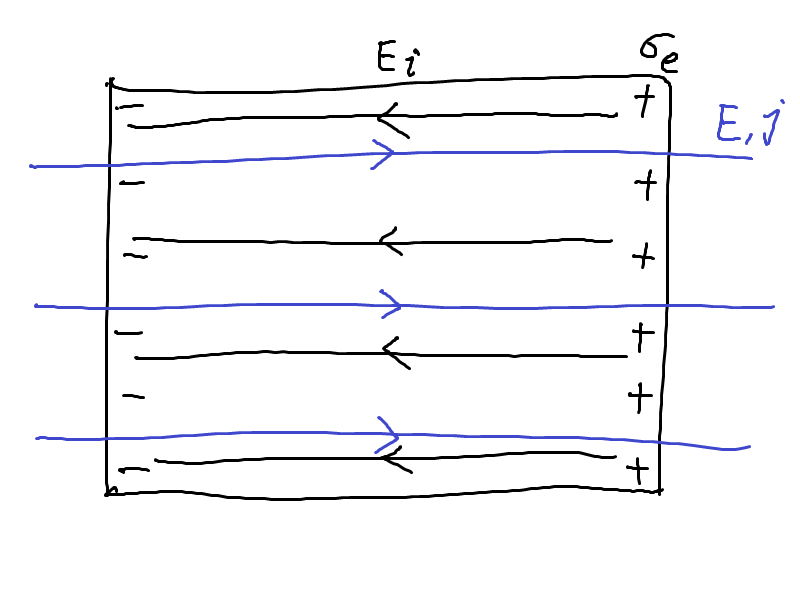
\includegraphics[scale=0.5]{fig/elec-equi.png}
\caption{吓得电荷都流过去了}
\label{fig-elec-equi}
\end{figure}

(高中学过的欧姆定律是$I=\frac{U}{R}$,而且$j=\frac{I}{S}$,$E=\frac{U}{l}$,$\rho=\frac{R S}{l}$,所以$j=\frac{E}{\rho}$,这是欧姆定律的微分形式)

导体的两边会积累电荷,电荷与电流的关系满足$\nabla \cdot \mathbf{j}=-\frac{\partial \rho_e}{\partial t}$,$\rho_e$是电荷密度。这就是电荷守恒定律的微分形式,表示某个点增加的电荷是从附近的电流流进来的。(你仍然可以检验一下两边量纲一样)

在导体的边界上,先看正电荷积累的一边,内侧有$j$流进去,而外侧没有,所以要把上面的方程改成$-j=-\frac{\opd \sigma_e}{\opd t}$,$\sigma_e$是电荷面密度。而负电荷积累的一边,内侧有$j$流出来,方程改成$j=-\frac{\opd (-\sigma_e)}{\opd t}$,跟正电荷那边一样。

这些电荷会产生反向的电场$E_i$,相当于一个平行板电容器,$E_i=\frac{\sigma_e}{\epsilon_0}$。

(高中学过电容器公式$C=\frac{S}{4 \pi k l}$,而且$\epsilon_0=\frac{1}{4 \pi k}$,$U=\frac{Q}{C}$,$E_i=\frac{U}{l}$,$\sigma_e=\frac{Q}{S}$,所以$E_i=\frac{\sigma_e}{\epsilon_0}$)

$E$和$E_i$都对电流有影响,刚才$j$的方程要改成$j=\frac{1}{\rho}(E-E_i)$。把上面的方程联立起来,得到$\sigma_e$满足的微分方程
\begin{equation*}
\frac{E}{\rho}-\frac{\sigma_e}{\epsilon_0 \rho}=\frac{\opd \sigma_e}{\opd t}
\end{equation*}

(如果你已经背出了它的解,可以跳过接下来的过程)令$x=\frac{E}{\rho}-\frac{\sigma_e}{\epsilon_0 \rho}$,$\opd x=-\frac{1}{\epsilon_0 \rho} \opd \sigma_e$,方程就变成了$x=-\epsilon_0 \rho \frac{\opd x}{\opd t}$,解得$x=x_0 \rme^{-\frac{t}{\epsilon_0 \rho}}$。

$t=0$时,$\sigma_e=0$,$x_0=\frac{E}{\rho}$,也就是$\frac{E}{\rho}-\frac{\sigma_e}{\epsilon_0 \rho}=\frac{E}{\rho} \rme^{-\frac{t}{\epsilon_0 \rho}}$,两边的电荷面密度$\sigma_e=\epsilon_0 E (1-\rme^{-\frac{t}{\epsilon_0 \rho}})$,总电场$E_s=E-E_i=E \rme^{-\frac{t}{\epsilon_0 \rho}}$。

可以看出,$t$很大时,$\sigma_e=\epsilon_0 E$,$E-E_i=0$,导体内没有电场。从数学上看,在有限的时间内,总电场只能无限接近零,而不可能严格为零。但是在一定的误差范围内,我们可以说它为零。

$\epsilon_0 \rho$的量纲是时间,所以把它称为特征时间$\tau$。每经过时间$\tau$,总电场就减小为$\frac{1}{e}$。

铜的电阻率$\rho=2 \times 10^{-8} \unit{\Omega \cdot m}$,所以$\tau=2 \times 10^{-19} \unit{s}$,电荷会迅速达到平衡。其他导体的$\tau$也差不多。
\section{磁单极子}
(这些东西只是为了好看放在这里)

假设磁单极子存在,用$q_m$表示它的磁荷。与电荷类比,它受到的洛伦兹力应该是$\mathbf{F}=q_m(\mathbf{B}-\frac{1}{c^2} \mathbf{v} \times \mathbf{E})$。$\frac{1}{c^2}$是为了凑量纲加上去的,负号则是为了让这个公式在洛伦兹变换下不变。可以看出,$q_m$的量纲是$[I] [T]$。

现在的麦克斯韦方程组是:
\begin{align*}
\nabla \cdot \mathbf{E}&=\frac{\rho_e}{\epsilon_0} & \nabla \cdot \mathbf{B}&=\mu_0 \rho_m \\
\nabla \times \mathbf{E}&=-\frac{1}{c^2} \frac{\mathbf{j}_m}{\epsilon_0}-\frac{\partial \mathbf{B}}{\partial t} & \nabla \times \mathbf{B}&=\mu_0 \mathbf{j}_e+\frac{1}{c^2} \frac{\partial \mathbf{E}}{\partial t}
\end{align*}

这样看起来就更有对称性了。正是从对称性考虑,许多理论都认为磁单极子应该存在,但是目前还没有实验能证明它存在。

(接下来我也不知道该讲什么了,可能要讲泊松方程和球坐标系下的分离变量,以及电磁场的能量、动量和角动量,还有辐射和天线的事情)

\chapter{统计力学}
\section{玻尔兹曼分布}
先考虑这样一个问题:假设空气的温度是均匀的,那么空气的密度和压强随高度怎么分布呢?

如图\ref{fig-air-block},在高度为$h$处取一小块底面积为$\Delta S$,高度为$\Delta h$的空气作为研究对象,设它的密度为$\rho$,那么它的质量就是$\rho \Delta S \Delta h$,上下受到的压强分别是$p(h+\Delta h)$和$p(h)$。
\begin{figure}[htb]
\centering
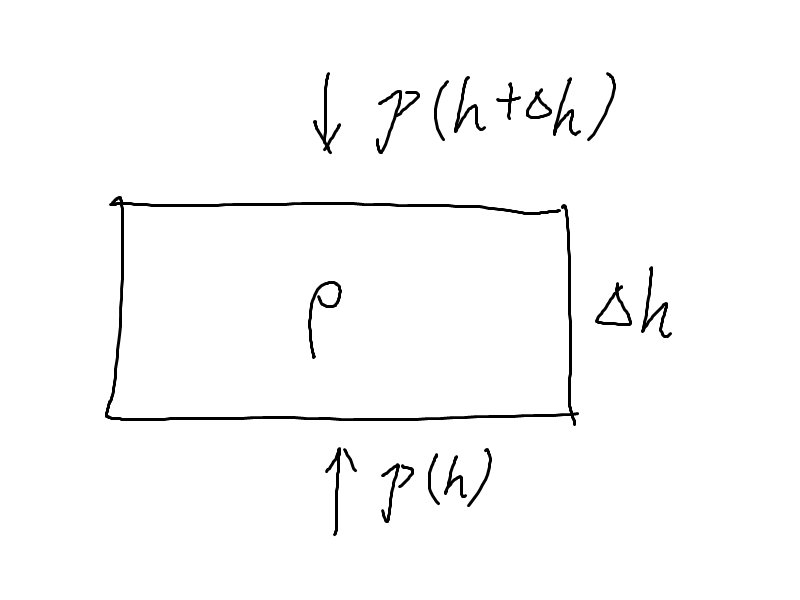
\includegraphics[scale=0.5]{fig/air-block.png}
\caption{一块空气}
\label{fig-air-block}
\end{figure}

这块空气受力平衡,$\rho \Delta S \Delta h g+p(h+\Delta h) \Delta S-p(h) \Delta S=0$,化简得$\rho g \Delta h+\Delta p=0$。

我们知道理想气体状态方程$p V=n R T$,另一种写法是$p \mu=\rho R T$,$\mu$是空气的平均相对分子质量,设它随高度是不变的。$R$叫作普适气体常量, $R \approx 8.31 \unit{J/(mol \cdot K)}$。两边微分得到$\Delta p \mu=\Delta \rho R T$。

(先不管差分算符$\Delta$和微分算符$\opd$的区别。$\rho(h)$和$p(h)$都是$h$的函数,有时候自变量省略不写)

合起来得到$\frac{\Delta \rho}{\rho}=-\frac{\mu g \Delta h}{R T}$,这是一个关于$\rho(h)$的微分方程,解得$\rho=\rho_0 \rme^{-\frac{\mu g h}{R T}}$。如果$h$是从地面开始算的,那么$\rho_0$就是地面处的空气密度。

温度$T$越高,比例系数$\frac{\mu g}{R T}$越小,指数衰减就越慢,也就是说分子(比温度低的时候)更容易出现在高的地方。(方便起见,这里把分子、原子之类的东西都叫作分子)

一个分子的质量$m=\frac{\mu}{N_A}$,玻尔兹曼常量$k=\frac{R}{N_A}$,所以上式也可以写成$\rho=\rho_0 \rme^{-\frac{m g h}{k T}}$。

代入$p$的式子得到$p=p_0 \rme^{-\frac{m g h}{k T}}$。同理可以得到分子数密度$\frac{\Delta N}{\Delta V}$也符合$\rme^{-\frac{m g h}{k T}}$的分布。也就是说,高度为$h$处出现一个分子的概率正比于$\rme^{-\frac{m g h}{k T}}$。设这个概率为$f_h(h)=A \rme^{-\frac{m g h}{k T}}$,$A$是一个比例系数,这就是分子高度的分布函数,叫作玻尔兹曼分布。

既然它是一个概率,那么各个地方出现分子的概率加起来必须等于$1$,也就是$\int_0^\infty f_h(h) \opd h=1$,所以$A=\frac{m g}{k T}$。这种乘上一个常数,让概率加起来等于$1$的方法叫作\emph{归一化}。
\section{麦克斯韦分布}
现在考虑分子速度的分布。速度有$x,y,z$三个分量,先考虑$z$分量。如果高度为$0$的地方有一个分子的$v_z$为$v_{z 0}$,那么它可以跑到高度为$\frac{v_{z 0}^2}{2 g}$的地方,并且$v_z$变为$0$。(只考虑重力作用,忽略分子之间的作用)

也就是说,$v_z$为$v_{z 0}$,高度为$0$的分子数等于$v_z$为$0$,高度为$\frac{v_{z 0}^2}{2 g}$的分子数。设分子的$v_z$和高度的分布函数为$f_{v_z,h}(v_z,h)$,那么$f_{v_z,h}(v_{z 0},0)=f_{v_z,h}(0,\frac{v_{z 0}^2}{2 g})$。

然后麦克斯韦做了一个假设:在不同的高度,分子的速率分布是相同的。如果高度为$1 \unit{m}$的分子中速度为$2 \unit{m/s}$的分子占了$10\%$,那么高度为$10 \unit{m}$的分子中速度为$2 \unit{m/s}$的分子也占$10\%$。因此分布函数可以表示为$f_{v_z,h}(v_z,h)=f_{v_z}(v_z) f_h(h)$,$f_{v_z}$和$f_h$是两个独立的分布函数,现在需要求出$f_{v_z}$。

$f_{v_z}(v_{z 0}) f_h(0)=f_{v_z}(0) f_h(\frac{v_{z 0}^2}{2 g})$,代入已知的$f_h$得到$f_{v_z}(v_{z 0})=f_{v_z}(0) \rme^{-\frac{m g}{k T} \frac{v_{z 0}^2}{2 g}}$,也就是说$f_{v_z}(v_z)=f_{v_z}(0) \rme^{-\frac{m v_z^2}{2 k T}}$。

现在$f_{v_z}(0)$相当于一个待定的比例系数,要让$\int_{-\infty}^\infty f_{v_z}(v_z) \opd v_z=1$。(刚才是从$0$积到$\infty$,因为分子的高度是从$0$开始算的;现在是从$-\infty$积到$\infty$,因为分子的$v_z$可正可负)

计算这个积分比较困难,这里直接给出结论:$\int_{-\infty}^\infty \rme^{-x^2} \opd x=\sqrt{\pi}$,所以$\int_{-\infty}^\infty f_{v_z}(0) \rme^{-\frac{m v_z^2}{2 k T}} \opd v_z=\sqrt{\pi} \sqrt{\frac{2 k T}{m}} f_{v_z}(0)$,$f_{v_z}(0)=\sqrt{\frac{m}{2 \pi k T}}$。

(现在这些奇怪的积分如果不会算没关系,也用不着背下来,会算一些最简单的积分就行了)

$f_{v_z}$只包含$v_z$的二次项,所以$+v_z$和$-v_z$对应的$f_{v_z}$是一样的。许多只与速度的大小有关,而与方向无关的东西可以用这一点来检查。

向各个方向运动的分子数是均匀的,所以$f_{v_x}$和$f_{v_y}$应该与$f_{v_z}$一样:$f_{v_x}(v_x)=\sqrt{\frac{m}{2 \pi k T}} \rme^{-\frac{m v_x^2}{2 k T}}$,$f_{v_y}(v_y)=\sqrt{\frac{m}{2 \pi k T}} \rme^{-\frac{m v_y^2}{2 k T}}$。

把它们乘起来得到$f_{v_x,v_y,v_z}(v_x,v_y,v_z)=(\frac{m}{2 \pi k T})^\frac{3}{2} \rme^{-\frac{1}{k T} \frac{1}{2} m (v_x^2+v_y^2+v_z^2)}$$=(\frac{m}{2 \pi k T})^\frac{3}{2} \rme^{-\frac{m v^2}{2 k T}}$,这就是分子速度(包括三个分量,或者说大小和方向)的分布函数。

前面的系数目前不是很重要,重要的是后面是一个指数衰减$\rme^{-\frac{m v^2}{2 k T}}$。

如果只考虑速度的大小(速率),可以取一个坐标轴为$v_x,v_y,v_z$的三维坐标系,把分子按照速度放在坐标系里。然后画一个以原点为中心,$v$为半径的球面,面积为$4 \pi v^2$。这个球面上的分子都满足速率为$v$,而球面上的每一点的分子数密度为$(\frac{m}{2 \pi k T})^\frac{3}{2} \rme^{-\frac{m v^2}{2 k T}}$,所以分子速率的分布函数$f_v(v)=4 \pi v^2 (\frac{m}{2 \pi k T})^\frac{3}{2} \rme^{-\frac{m v^2}{2 k T}}$。这就是麦克斯韦速率分布。

如果分子的坐标是$x,y,z$,对应的速度是$\dot x,\dot y,\dot z$,那么把坐标的分布函数和速度的分布函数乘起来就能得到“坐标和速度”的分布函数$f(x,y,z,\dot x,\dot y,\dot z)=\frac{m g}{k T} (\frac{m}{2 \pi k T})^\frac{3}{2} \rme^{-\frac{1}{k T} (\frac{1}{2} m (\dot x^2+\dot y^2+\dot z^2)+m g z)}$。
\section{分布函数}
可以发现,分子高度的分布函数有一项$\rme^{-\frac{m g h}{k T}}$,速度的分布函数有一项$\rme^{-\frac{m v^2}{2 k T}}$。现在可以猜:如果一个分子的坐标是$q$(多个坐标的情况类似),速度是$\dot q$,能量是$E(q,\dot q)$,那么分布函数就是$f(q,\dot q)=A \rme^{-\frac{E}{k T}}$,$A$是归一化系数。

如果一个系统(专业一点叫\emph{系综})里有很多一样的分子,忽略这些分子之间的相互作用,并且系统达到热平衡,那么从里面随便取一个分子,它的坐标为$q_0$,速度为$\dot q_0$的概率就是$f(q_0,\dot q_0)$。可以看出,温度越高,指数衰减越慢,分子越容易具有较高的能量。

(现在把这一点当作基本假设,但是严格的统计力学是用别的基本假设推出它的。而且它只对温度和分子数恒定的系统成立)

什么叫热平衡?这个问题现在先不仔细讲。在空气的例子中,热平衡就是各处的温度相同,而且随便取一小块空气都受力平衡。系统要达到热平衡,那么分子之间的相互作用不可能完全为零,否则热量就不能从一部分传到另一部分。分子之间的相互作用不可忽略,或者系统没有达到热平衡的情况比较复杂,我们也不仔细讲。
\section{统计平均值}
知道分布函数之后,可以算出分子微观性质的统计平均值,它就是物质的宏观性质。

比如空气的例子中,我们来计算分子的平均高度:$\overline{h}=\int_0^\infty h f_h(h) \opd h=\int_0^\infty h \frac{m g}{k T} \rme^{-\frac{m g h}{k T}} \opd h$。这个积分我们可以学一下:
\begin{align*}
\int_0^\infty x \rme^{-x} \opd x&=\int_0^\infty x \cdot (-\opd \rme^{-x}) \\
&=\left. -x \rme^{-x} \right|_0^\infty-\int_0^\infty (-\rme^{-x}) \opd x \\
&=\left. -x \rme^{-x} \right|_0^\infty-\left. \rme^{-x} \right|_0^\infty \\
&=1
\end{align*}

令$x=\frac{m g h}{k T}$,得到$\overline{h}=\frac{k T}{m g}$。还可以算出平均重力势能$\overline{E}=\int_0^\infty m g h f_h(h) \opd h=k T$。这是从地面到无穷高处的空气的平均重力势能,而且作了很多并不实际的简化。一般我们考虑一个小容器里的气体时,重力势能是忽略的。

只考虑分子在$x$方向上的运动,可以计算平均动能:$\overline{E_{k x}}=\int_{-\infty}^\infty \frac{1}{2} m v_x^2 f_{v_x}(v_x) \opd v_x$。计算这个积分也比较困难,这里直接给出结论:$\overline{E_{k x}}=\frac{1}{2} k T$。

类似地有$\overline{E_{k x}}=\overline{E_{k y}}=\frac{1}{2} k T$,三维空间中的平均动能$\overline{E_k}=\frac{3}{2} k T$。也就是说,每个平动自由度对应着$\frac{1}{2} k T$的平均动能。

一摩尔气体的能量$E_\text{mol}=N_A \overline{E_k}=\frac{3}{2} R T$。它的比热是升高单位温度需要的能量,所以比热$C_\text{mol}=\frac{\opd E_\text{mol}}{\opd T}=\frac{3}{2} R$。对于只能平动,不能转动的单原子分子,这个结果与实验基本符合,更精确的结果需要考虑量子效应。
\section{量子谐振子}
上面考虑的都是坐标和能量可以连续分布的情况,但是在量子力学中,能量是离散(不连续)分布的,这时把上面的积分改成求和就行了。

固体里的分子在平衡位置附近振动,它们的能量可以取$\hbar \omega,2 \hbar \omega,3 \hbar \omega,\dots$,$\hbar \omega$是一个单位的能量。分子的能量为$n \hbar \omega$的概率$f(n)=A \rme^{-\frac{n \hbar \omega}{k T}}$。

然后确定$A$:$\sum_{n=1}^\infty f(n)=A \frac{\rme^{-\frac{\hbar \omega}{k T}}}{1-\rme^{-\frac{\hbar \omega}{k T}}}$(高考范围内的等比数列求和),而$\sum_{n=1}^\infty f(n)=1$,所以$A=\rme^{\frac{\hbar \omega}{k T}}-1$。

计算一个振子的平均能量:
\begin{align*}
\overline{E}&=\sum_{n=1}^\infty n \hbar \omega f(n) \\
&=A k T \sum_{n=1}^\infty \frac{n \hbar \omega}{k T} \rme^{-\frac{n \hbar \omega}{k T}} \\
&=A k T \frac{\hbar \omega}{k T} \frac{\rme^{-\frac{\hbar \omega}{k T}}}{(1-\rme^{-\frac{\hbar \omega}{k T}})^2} \\
&=\frac{\hbar \omega}{1-\rme^{-\frac{\hbar \omega}{k T}}}
\end{align*}

($\sum n \rme^{-n}$这样的求和应该也是高考范围内的,但是它有一种黑科技的计算方法:先算出$\sum \rme^{-n x}$,然后发现$\sum n \rme^{-n}=-\left. \ddx \sum \rme^{-n x} \right|_{x=1}$。类似的黑科技在后面数列那一章会讲)

一个振子的比热
\begin{equation*}
C=\frac{\opd \overline{E}}{\opd T}=k (\frac{\hbar \omega}{k T})^2 \frac{\rme^{-\frac{\hbar \omega}{k T}}}{(1-e^{-\frac{\hbar \omega}{k T}})^2}
\end{equation*}

比热随温度的变化如图\ref{fig-quant-osc-c}:
\begin{figure}[htb]
\centering
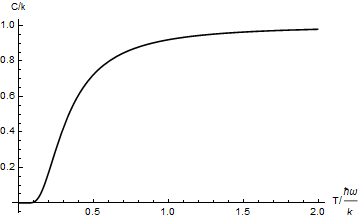
\includegraphics[scale=0.5]{fig/quant-osc-c.png}
\caption{越来越热的时候}
\label{fig-quant-osc-c}
\end{figure}

我们知道$\hbar$很小,而一般情况下$T$很大(物理学中的温度一般是开尔文而不是摄氏度),也就是说$\frac{\hbar \omega}{k T} \ll 1$,$\rme^{-\frac{\hbar \omega}{k T}}=1-\frac{\hbar \omega}{k T}$,做一些小量运算可以得到$\overline{E}=k T$,$C=k$,这与经典理论(比如刚才空气按高度分布)是一致的。如果温度很低,就要考虑量子效应。

总而言之,统计力学就是先想办法确定系统的分布函数,然后计算分子微观性质的统计平均值,得到物质的宏观性质。比如很多电荷定向移动形成电流,很多有磁性的分子有序排列形成磁铁。从力学观点来看,每个分子的运动决定了物质宏观的运动,但是分子太多了,不可能一个个去解它们的运动方程。然而正是因为分子数很多,可以用统计规律来处理它们。

\chapter{量子力学}
\rightline{\it 不要自学量子力学。}
\section{薛定谔方程}
我们先来看看传说中的薛定谔方程:
\begin{equation*}
\rmi \hbar \ppt \psi=H \psi
\end{equation*}

它是量子力学最基本的规律,表示系统随着时间的变化,就像牛顿力学中的$F=m a$一样。

$\psi$是系统的波函数,它可以是复数或者矩阵之类的。量子力学用波函数来描述系统的状态,就像牛顿力学用质点的位置之类的来描述系统的状态一样。

($\psi$的英文写法是psi,传说应该读作赛,p不发音,就像$\pi$读作派,$\phi$读作fài一样)

$H$叫作哈密顿算符。它并不是一个普通的数乘到$\psi$上面,$H \psi$其实是一个函数$H(\psi)$,但是出于习惯,直接用乘法来表示。$H$可以包含求导之类的操作,也可以是矩阵。薛定谔方程并不能告诉我们一个系统的$H$是什么,需要用其他方法推导出来。
\section{氨分子双态系统;定态}
氨分子有一个氮原子和三个氢原子,氮原子可以在氢原子的上面或者下面,称为状态$1$和状态$2$,如图\ref{fig-ammonia}。
\begin{figure}[htb]
\centering
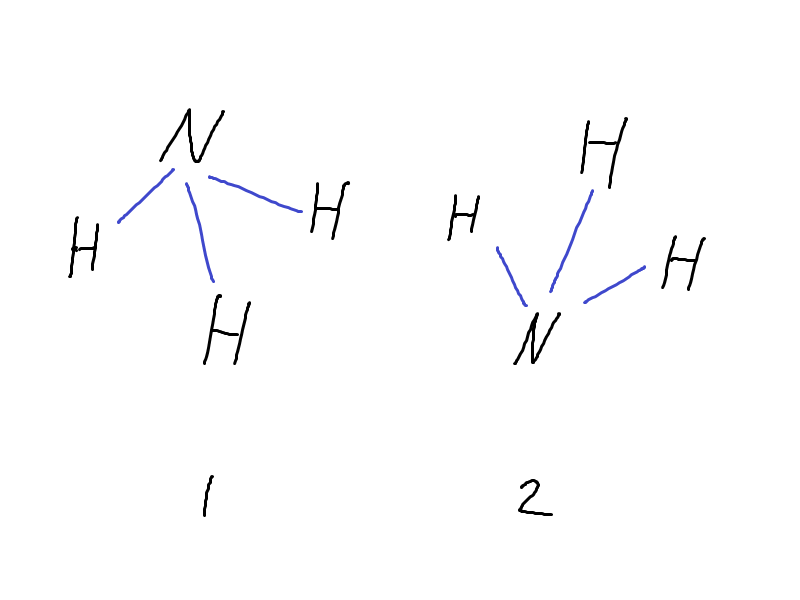
\includegraphics[scale=0.5]{fig/ammonia.png}
\caption{活泼可爱的氨分子}
\label{fig-ammonia}
\end{figure}

简单起见,假设氨分子不能移动或者转动,但是因为一些量子效应,它可以上下翻转。

氨分子的波函数是一个二维矢量:$\mathbf{\psi}=\begin{bmatrix} \psi_1 \\ \psi_2 \end{bmatrix}$。$\psi_1$和$\psi_2$分别表示它处于状态$1$和状态$2$的概率幅,它们都是复数。这里说的概率幅并不是概率,具体待会再讲。

而它的$H$是一个矩阵:$\mathbf{H}=\begin{bmatrix} E_0 & \Delta E \\ \Delta E & E_0 \end{bmatrix}$。$E_0$是氨分子的能量,就是把几根化学键的键能加起来得到的能量。$\Delta E$表示翻转所减少的能量,$\Delta E$越大,翻转就越容易。为什么$H$是这样,也要待会才能明白。

现在来看薛定谔方程:$\rmi \hbar \ppt \mathbf{\psi}=\mathbf{H} \psi$,前面已经知道它的解可以直接写成$\mathbf{\psi}=\rme^{-\rmi \frac{t}{\hbar} \mathbf{H}} \mathbf{\psi_0}$,但是这么写并没有什么用。我们要分别解出$\psi_1$和$\psi_2$关于时间的函数,因此把这个矩阵方程写成两个标量方程:
\begin{align*}
\rmi \hbar \ppt \psi_1&=E_0 \psi_1+\Delta E \psi_2 & \rmi \hbar \ppt \psi_2&=\Delta E \psi_1+E_0 \psi_2
\end{align*}

先把问题再简化一点,假设氨分子连上下翻转的量子效应都没有,也就是$\Delta E=0$,那么
\begin{align*}
\rmi \hbar \ppt \psi_1&=E_0 \psi_1 & \rmi \hbar \ppt \psi_2&=E_0 \psi_2
\end{align*}

可以直接解出$\psi_1=\psi_{1 0} \rme^{-\rmi \frac{E_0}{\hbar} t}$,$\psi_2=\psi_{2 0} \rme^{-\rmi \frac{E_0}{\hbar} t}$,$\psi_{1 0}$和$\psi_{2 0}$是待定的初始条件。

量子力学的另一条基本假设是:我们可以用实验测量一个氨分子在状态$1$还是状态$2$,在某个状态的概率为概率幅的模长的平方。比如在状态$1$的概率$P_1=|\psi_1|^2=\psi_1 \psi_1^*=\psi_{1 0}^2$。$\psi_1$的模长是不变的,所以$P_1$与时间无关,这样的波函数叫作定态。在状态$2$的概率则是$P_2=\psi_{2 0}^2$。既然它是一个概率,那么$P_1+P_2=1$,对初始条件的要求就是$\psi_{1 0}^2+\psi_{2 0}^2=1$。
\section{氨分子振荡;中微子振荡}
只有定态就太无聊了,现在来考虑氨分子的翻转。把上面的方程一加一减,得到
\begin{align*}
\rmi \hbar \ppt (\psi_1+\psi_2)&=(E_0+\Delta E)(\psi_1+\psi_2) & \rmi \hbar \ppt (\psi_1-\psi_2)&=(E_0-\Delta E)(\psi_1-\psi_2)
\end{align*}

可以直接解出$(\psi_1+\psi_2)=(\psi_{1 0}+\psi_{2 0}) \rme^{-\rmi \frac{E_0+\Delta E}{\hbar} t}$,$(\psi_1-\psi_2)=(\psi_{1 0}-\psi_{2 0}) \rme^{-\rmi \frac{E_0-\Delta E}{\hbar} t}$。

不妨设初始时氨分子一定在状态$1$,$\psi_1=1$,$\psi_2=0$。那么
\begin{align*}
\psi_1&=\frac{1}{2}((\psi_{1 0}+\psi_{2 0}) \rme^{-\rmi \frac{E_0+\Delta E}{\hbar} t}+(\psi_{1 0}-\psi_{2 0}) \rme^{-\rmi \frac{E_0-\Delta E}{\hbar} t}) \\
&=\frac{1}{2}(\rme^{-\rmi \frac{E_0+\Delta E}{\hbar} t}+\rme^{-\rmi \frac{E_0-\Delta E}{\hbar} t}) \\
&=\frac{1}{2}(\rme^{-\rmi \frac{\Delta E}{\hbar} t}+\rme^{+\rmi \frac{\Delta E}{\hbar} t}) \rme^{-\rmi \frac{E_0}{\hbar} t} \\
&=\cos (\frac{\Delta E}{\hbar} t) \rme^{-\rmi \frac{E_0}{\hbar} t}
\end{align*}
\begin{figure}[htb]
\centering
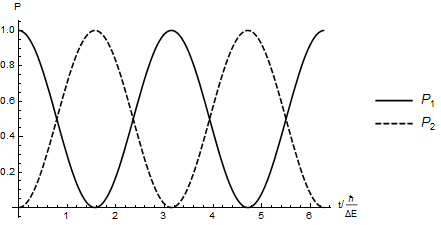
\includegraphics[scale=0.5]{fig/ammonia-osc.png}
\caption{氨分子转起来了}
\label{fig-ammonia-osc}
\end{figure}

同理可得$\psi_2=-\rmi \sin (\frac{\Delta E}{\hbar} t) \rme^{-\rmi \frac{E_0}{\hbar} t}$。$P_1=\cos^2 (\frac{\Delta E}{\hbar} t)$,$P_2=\sin^2 (\frac{\Delta E}{\hbar} t)$,如图\ref{fig-ammonia-osc}。可以看出,随着时间的推移,氨分子在不断翻转,而且始终满足$P_1+P_2=1$。恭喜你!你已经会用量子力学来解决问题了!

$\Delta E$越大,氨分子翻转得越快。翻转一次需要的时间$\tau=\frac{\hbar}{\Delta E}$,它有时间的量纲,至于$2 \pi$之类的系数在这里并不重要。

前几年有一个热门的东西叫中微子振荡。中微子分为三种:电子中微子、$\mu$子中微子、$\tau$子中微子,分别用$\nu_e$、$\nu_\mu$、$\nu_\tau$表示。它们可以互相转化,比如一个$\nu_e$飞着飞着就会变成$\nu_\mu$,原理和上面的氨分子振荡差不多。在$\nu_e$和$\nu_\mu$之间振荡的周期$T=\frac{\hbar}{E_{\nu_\mu}-E_{\nu_e}}$,$E_{\nu_e}$和$E_{\nu_\mu}$分别是$\nu_e$和$\nu_\mu$的能量。

中微子的质量很小,至今都不能确定它是否为零。我们可以测出振荡周期,然后算出中微子的能量,接着算出质量,这是测量中微子质量的方法之一。
\section{能级分裂}
在上面的例子中,如果设$\psi_+=\psi_1+\psi_2$,$\psi_-=\psi_1-\psi_2$,那么它们都是定态:$\psi_+=\psi_{+ 0} \rme^{-\rmi \frac{E_0+\Delta E}{\hbar} t}$,$\psi_-=\psi_{- 0} \rme^{-\rmi \frac{E_0-\Delta E}{\hbar} t}$。

我们可以用实验测量一个氨分子在状态$1$还是状态$2$,也可以用另外的实验测量一个氨分子在状态$+$还是状态$-$。知道了状态$1$和状态$2$的概率幅,就能确定系统的波函数;知道了状态$+$和状态$-$的概率幅,也能确定系统的波函数,相当于选取不同的坐标(专业一点叫\emph{表象})来描述这个系统。

但是状态$+$和状态$-$是什么东西呢?用氨分子的例子可能比较难理解,先看这样一个例子:有两个相同的单摆,用一根弹簧相连,如图\ref{fig-spring-pend}。我们可以让左边的摆单独摆动,也可以让右边的摆单独摆动,分别叫作状态$1$和状态$2$。
\begin{figure}[htb]
\centering
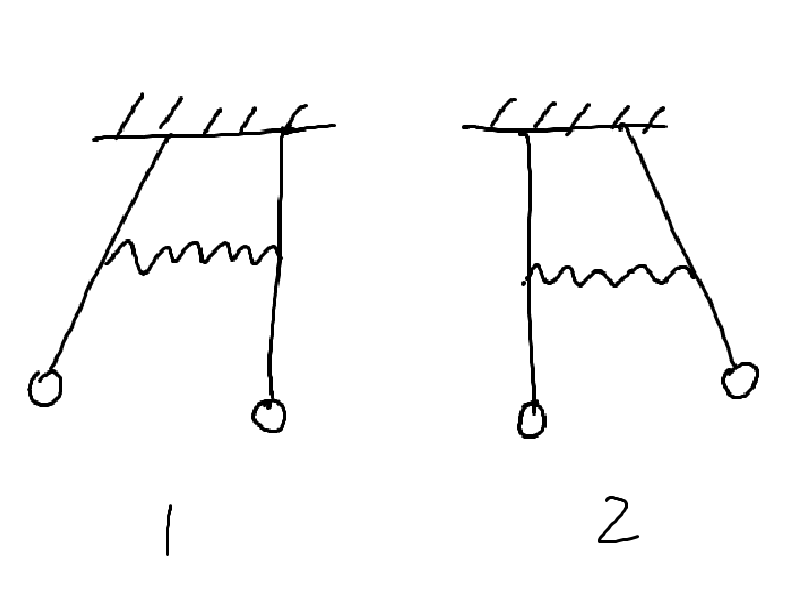
\includegraphics[scale=0.5]{fig/spring-pend.png}
\caption{活泼可爱的弹簧摆}
\label{fig-spring-pend}
\end{figure}

但是我们也可以让两个摆一起摆动,有两种不同的方式,如图\ref{fig-spring-pend-2},相当于刚才的状态$+$和状态$-$。系统的任何运动都可以看作状态$1$和状态$2$的叠加,也可以看作状态$+$和状态$-$的叠加。
\begin{figure}[htb]
\centering
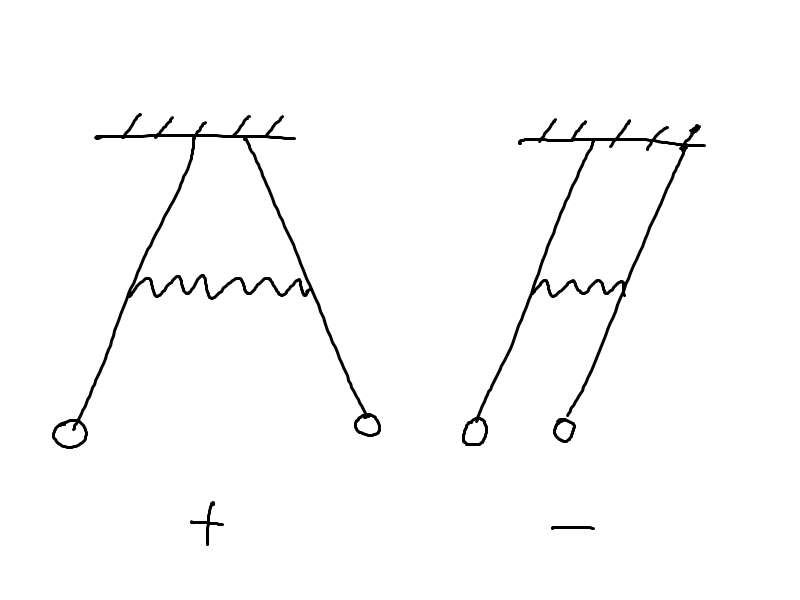
\includegraphics[scale=0.5]{fig/spring-pend-2.png}
\caption{弹簧摆在干奇怪的事情}
\label{fig-spring-pend-2}
\end{figure}

我们还可以选取更加奇怪的坐标来描述这个系统,但是状态$+$和状态$-$有一个好处:它们是定态,或者说它们的运动方程互相独立。学到后面就会发现定态会带来计算上的方便。

回到氨分子的例子,状态$+$的相位是$\rme^{-\rmi \frac{E_0+\Delta E}{\hbar} t}$,而不是$\rme^{-\rmi \frac{E_0}{\hbar} t}$。因此可以认为状态$+$的能量是$E_0+\Delta E$,同理状态$-$的能量是$E_0-\Delta E$。虽然状态$1$和状态$2$的能量是一样的,但是因为它们可以翻转,产生了一个能量较高的状态和一个能量较低的状态,这种现象称为\emph{能级分裂}。

如果考虑一些统计力学的知识,我们还会发现,如果很多氨分子相互作用达到热平衡,会有比较多的氨分子喜欢待在能量较低的状态$-$。(事实上$\frac{P_-}{P_+}=\rme^{\frac{2 \Delta E}{k T}}$,具体的计算非常困难,但是这个结论符合直觉)

高中化学课可能讲过,原子的电子云重叠的时候会出现一条高能量轨道和一条低能量轨道,原理和这个差不多。
\section{一维无限深方势阱}
现在我们把一个粒子装在箱子里。粒子的$\psi$是一个复数,在一维情况下,它是位置和时间的函数$\psi(x,t)$。这里的位置和时间都是连续分布的。(如果不是连续分布的就可以写成矩阵)

粒子的$H=-\frac{\hbar^2}{2 m} \ppxn{2}+V(x)$,其中$-\frac{\hbar^2}{2 m} \ppxn{2}$相当于动能,$V(x)$相当于势能。待会再讲它是怎么来的,现在先用它来算一些有意思的东西。

如果箱子的长度为$a$,$V(x)$可以表示为(分界点的等号不用在意)
\begin{equation*}
V(x)=\begin{cases}
0, &0<x<a \\
\infty, &x<0\text{或}x>a
\end{cases}
\end{equation*}

这样的势能叫作无限深方势阱。$0<x<a$范围内势能为$0$,外面的势能为$\infty$,所以说它是无限深的。从$0$过渡到$\infty$的图像是一条竖直线,所以说它是方的。注意它是一个一维的函数。

现在来解薛定谔方程:
\begin{equation*}
\rmi \hbar \ppt \psi=-\frac{\hbar^2}{2 m} \ppxn{2} \psi+V(x) \psi
\end{equation*}

在势阱里面,$V(x)=0$,这是一个齐次方程。正常的量子力学课本会用分离变量法解这个方程,但是我们只要猜解就行了。我们猜:$\psi=A \rme^{\rmi(k x-\omega t)}$。

($A$仍然是待定的常量。$k$叫作波数,它的量纲与$\frac{1}{x}$相同,不要和弹簧的劲度系数搞混。出于习惯,$\omega$前面有个负号,如果学了相对论会更清楚原因)

代入方程得到$\rmi \hbar \cdot -\rmi \omega \psi=-\frac{\hbar^2}{2 m} \cdot -k^2 \psi$,$\omega=\frac{\hbar k^2}{2 m}$。这就是$\omega$和$k$必须满足的关系。

在势阱外面,无穷大的势能与$\psi$相乘,所以$\psi$必须等于$0$。因此可以把$A$相等,$k$互为相反数的两个解叠加:$\psi=A (\rme^{\rmi(k x-\omega t)}-\rme^{\rmi(-k x-\omega t)})=2 \rmi A \sin(k x) \rme^{-\rmi \omega t}$。它满足边界条件:$x=0$时,$\psi=0$。(如果叠加的时候是$\rme^{\rmi(k x-\omega t)}+\rme^{\rmi(-k x-\omega t)}$,就不满足这个条件)

另一个边界条件是$x=a$时,$\psi=0$,因此$\sin(k a)=0$,$k=\frac{n \pi}{a}(n=1,2,3,\dots)$。(如果$n=0$,$\psi$就恒为$0$,没有物理意义。后面还会发现$n$为负数的情况是没用的)

所以,$\omega=\frac{n^2 \pi^2 \hbar}{2 a^2 m}$,$\psi=A' \sin(\frac{n \pi}{a} x) \rme^{-\rmi \frac{n^2 \pi^2 \hbar}{2 a^2 m} t}$,其中$A'=2 \rmi A$。

这是粒子在时间$t$出现在位置$x$的概率幅,别忘了概率是概率幅的模长的平方:$P=\psi \psi^*=A'^2 \sin^2 (\frac{n \pi}{a} x)=A'^2 \frac{1}{2} (1-\cos(\frac{2 n \pi}{a} x))$。

这个概率必须归一化:$\int_0^a P \opd x=1$(计算这个积分可以用倍角公式),所以$A'=\sqrt{\frac{2}{a}}$,$P=\frac{2}{a} \sin^2 (\frac{n \pi}{a} x)=\frac{1}{a} (1-\cos(\frac{2 n \pi}{a} x))$,这就是粒子位置的概率分布。$n=1,2,3$时,$P(x)$如图\ref{fig-square-well}。
\begin{figure}[htb]
\centering
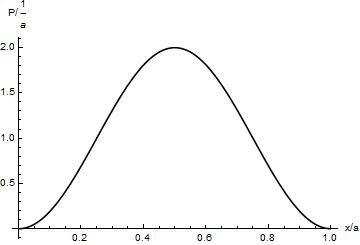
\includegraphics[scale=0.4]{fig/square-well.png}
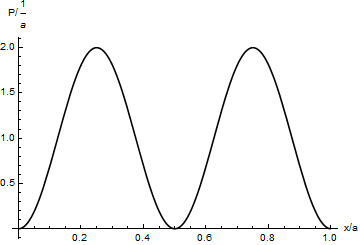
\includegraphics[scale=0.4]{fig/square-well-2.png}
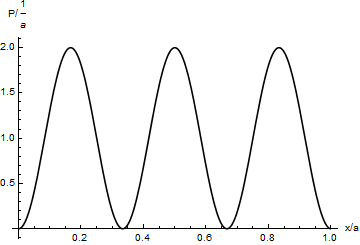
\includegraphics[scale=0.4]{fig/square-well-3.png}
\caption{粒子在方势阱里的位置分布}
\label{fig-square-well}
\end{figure}

前面说过$\rme^{-\rmi \omega t}$中的$\omega=\frac{E}{\hbar}$,所以粒子的能量$E=\hbar \omega=\frac{n^2 \pi^2 \hbar^2}{2 a^2 m}$。我们从小就知道,量子力学当中的能量不能连续变化,只能取不连续的值,这是微分方程的解所要求的。

可以看出,$n$越大,$E$就越大,粒子越容易跑到势阱中的各个地方,而$n$小的时候粒子不容易跑到势阱的边上。$\hbar$是一个很小的量,我们平常接触到的能量对应的$n$很大,所以没有明显的量子效应。

粒子位置的统计平均$\overline{x}=\int_0^a x P(x) \opd x=\frac{a}{2}$(先用倍角公式,然后拆成奇函数和偶函数),这个结果符合直觉。

$\psi$的量纲与$x^{-\frac{1}{2}}$相同,这样才能让$\int_{-\infty}^{\infty} \psi \psi^* \opd x=1$,右边是概率,是一个无量纲的数。现在你可以检查一下上面式子的量纲。在其他问题中,$\psi$的自变量不同,量纲也会不同。
\section{动量;动量算符}
粒子的平均位置$\overline{x}=\int_{-\infty}^{\infty} x \psi \psi^* \opd x$,但是我们一般写成$\int_{-\infty}^{\infty} \psi^* x \psi \opd x$。

粒子的平均速度是什么呢?在波函数中只有位置,没有速度,但是我们可以定义平均速度$\overline{v}=\frac{\opd \overline{x}}{\opd t}$。然后进行一些计算:(前方高能,看不懂可以先跳过)
\begin{align*}
\overline{v}&=\opdt \int_{-\infty}^{\infty} \psi^* x \psi \opd x \\
&=\int_{-\infty}^{\infty} \ppt(\psi^* x \psi) \opd x
\internote{(为什么要把$\opdt$变成$\ppt$呢?如果有一个函数$f(x,t)$,它的全微分$\opd f=\frac{\partial f}{\partial x} \opd x+\frac{\partial f}{\partial t} \opd t$,$\frac{\opd f}{\opd t}=\frac{\partial f}{\partial x} \frac{\opd x}{\opd t}+\frac{\partial f}{\partial t}$。这里$x$和$t$是独立的变量,$\frac{\opd x}{\opd t}=0$。如果$x$与$t$有关,就不能这样了。)}
&=\int_{-\infty}^{\infty} x \psi^* \ppt \psi+x \psi \ppt \psi^* \opd x
\end{align*}

我们要把$\psi^* \ppt \psi+\psi \ppt \psi^*$变成对$x$的微分,然后对$x$积分才方便。按照薛定谔方程:
\begin{align*}
\ppt \psi&=-\frac{\rmi}{\hbar} H \psi \\
&=-\frac{\rmi}{\hbar}(-\frac{\hbar^2}{2 m}\ppxn{2} \psi+V \psi) \\
&=\frac{\rmi \hbar}{2 m} \ppxn{2} \psi-\frac{\rmi}{\hbar} V \psi
\end{align*}

共轭项则是$\ppt \psi^*=-\frac{\rmi \hbar}{2 m} \ppxn{2} \psi^*+\frac{\rmi}{\hbar} V \psi^*$。

所以$\psi^* \ppt \psi+\psi \ppt \psi^*$中含有$V$的项会消掉,剩下$\frac{\rmi \hbar}{2 m}(\psi^* \ppxn{2} \psi-\psi \ppxn{2} \psi^*)$,它还可以写成$\frac{\rmi \hbar}{2 m} \ppx(\psi^* \ppx \psi-\psi \ppx \psi^*)$。

现在可以继续算$\overline{v}$,利用分部积分:
\begin{align*}
\overline{v}&=\frac{\rmi \hbar}{2 m} \int_{-\infty}^{\infty} x \ppx(\psi^* \ppx \psi-\psi \ppx \psi^*) \opd x \\
&=-\frac{\rmi \hbar}{2 m} \int_{-\infty}^{\infty} (\psi^* \ppx \psi-\psi \ppx \psi^*) \opd x \\
&=-\frac{\rmi \hbar}{2 m} \int_{-\infty}^{\infty} (\psi^* \ppx \psi+\psi^* \ppx \psi) \opd x \\
&=\int_{-\infty}^{\infty} \psi^* (-\frac{\rmi \hbar}{m} \ppx) \psi \opd x
\end{align*}

如果定义粒子的平均动量$\overline{p}=m \overline{v}$,那么$\overline{p}=\int_{-\infty}^{\infty} \psi^* (-\rmi \hbar \ppx) \psi \opd x$,就是把平均位置中的$x$换成了$-\rmi \hbar \ppx$。$-\rmi \hbar \ppx$称为动量算符,用$\hat{p}$表示。还可以定义位置算符$\hat{x}$就是$x$。

(量子力学经常研究动量,而不是速度。神奇的是,位置与动量的乘积的量纲与$\hbar$相同。)

如果粒子在位置$x$处的概率为$P(x)=\psi(x) \psi^*(x)$,动量为$p(x)$,那么(对位置的)平均动量就是$\overline{p}=\int_{-\infty}^{\infty} \psi^* p \psi$。然而在量子力学中,我们不能确定粒子在某个位置的动量$p(x)$。如果要计算平均动量,可以对$\hat{p}$“计算平均值”。接下来还会讲确定动量的概率分布的方法。

$\hat{p}$并不是一个函数,前面说过,它是一种把一个函数变成另一个函数的变换操作。只有在它的右边“乘”上一个函数,也就是对这个函数求导,才能得到另一个函数。

现在就知道粒子的$H=-\frac{\hbar^2}{2 m} \ppxn{2}+V$是怎么来的了:在牛顿力学中,动能为$\frac{1}{2} m v^2=\frac{p^2}{2 m}$,如果把$p$换成$\hat{p}$,就是$\frac{\hat{p}^2}{2 m}=-\frac{\hbar^2}{2 m} \ppxn{2}$,这一项代表动能。$V$则代表势能,加起来就是总能量。然而出于习惯,我们用$H$而不是$\hat{E}$表示能量,把它叫作哈密顿算符。

刚才算出了粒子在一维无限深方势阱中的定态波函数:
\begin{equation*}
\psi=\sqrt{\frac{2}{a}} \sin(\frac{n \pi}{a} x) \rme^{-\rmi \frac{n^2 \pi^2 \hbar}{2 a^2 m} t}, 0<x<a
\end{equation*}

现在我们假装认真地算一下它的平均动量:
\begin{align*}
\ppx \psi&=\frac{n \pi}{a} \sqrt{\frac{2}{a}} \cos(\frac{n \pi}{a} x) \rme^{-\rmi \frac{n^2 \pi^2 \hbar}{2 a^2 m} t} \\
\psi^* (-\rmi \hbar \ppx) \psi&=-\frac{2 \rmi n \pi \hbar}{a^2} \sin(\frac{n \pi}{a} x) \cos(\frac{n \pi}{a} x) \\
&=-\frac{\rmi n \pi \hbar}{a^2} \sin(\frac{2 n \pi}{a} x) \\
\overline{p}&=\int_{0}^{a} \psi^* (-\rmi \hbar \ppx) \psi \opd x \\
&=-\frac{\rmi \hbar}{2 a}(1-\cos(2 n \pi)) \\
&=0
\end{align*}

上面已经算过$\overline{x}=\frac{a}{2}$,与$x$无关,其实可以直接知道$\overline{p}=m \frac{\opd \overline{x}}{\opd t}=0$。

(这个定态的栗子好像举得很无聊,然而不是定态的话有很大的计算量)
\section{动量与傅立叶变换}
(因为章节安排的一些问题,这一节要看过后面的傅立叶变换才能看)

在讲氨分子的时候,可以用状态$1$和$2$描述氨分子的状态,也可以用状态$+$和$-$来描述,这两种方法相当于不同的坐标系,专业一点叫\emph{表象}。刚才用位置和时间描述粒子的状态,现在还可以用动量和时间来描述,也就是把位置表象下的波函数$\psi(x,t)$变换成动量表象下的波函数$\phi(p,t)$。($\psi$和$\phi$这两个字母容易搞混,但是很多人都在这么写)

$\psi(x,t)$可以分解为简谐波$\rme^{\rmi(k x-\omega t)}=\rme^{\rmi k x} \rme^{-\rmi \omega t}$(先不管振幅),$k$是波数,动量$p=\hbar k$。也就是说,动量表象就是位置表象的频谱,再乘上一些系数$\hbar$,而时间的部分不用变。

($p=\hbar k$和$E=\hbar \omega$这两个公式看起来很对称,高中学的应该是$p=\frac{h c}{\lambda}$和$E=h \nu$)

傅立叶变换的公式是:
\begin{align*}
g(k)&=\mathscr{F}_{x \rightarrow k} f(x)=\frac{1}{\sqrt{2 \pi}} \int_{-\infty}^{\infty} f(x) \rme^{-\rmi k x} \opd x &
f(x)&=\mathscr{F}^{-1}_{x \rightarrow k} g(k)=\frac{1}{\sqrt{2 \pi}} \int_{-\infty}^{\infty} g(k) \rme^{\rmi k x} \opd k
\end{align*}

乘上一些$\hbar$(可以通过换元,也可以凑量纲),就得到表象变换的公式:
\begin{align*}
\phi(p,t)&=\sqrt{\hbar} \mathscr{F}_{x \rightarrow \frac{p}{\hbar}} \psi(x,t) & \psi(x,t)&=\frac{1}{\sqrt{\hbar}} \mathscr{F}^{-1}_{x \rightarrow \frac{p}{\hbar}} \phi(p,t) \\
&=\frac{1}{\sqrt{2 \pi \hbar}} \int_{-\infty}^{\infty} \psi(x,t) \rme^{-\frac{\rmi}{\hbar} p x} \opd x & &=\frac{1}{\sqrt{2 \pi \hbar}} \int_{-\infty}^{\infty} \phi(p,t) \rme^{\frac{\rmi}{\hbar} p x} \opd p
\end{align*}

如果$\psi$已经归一化,那么$\phi$仍然是归一化的:$\int_{-\infty}^{\infty} \phi \phi^* \opd p=1$。粒子动量为$p$的概率$P=\phi \phi^*$。别忘了$\psi(x,t)$的量纲与$x^{-\frac{1}{2}}$相同,而$\phi(p,t)$的量纲与$p^{-\frac{1}{2}}$相同。

我们把这个公式凑出来了,然而具体的计算是很困难的。比如刚才的波函数:
\begin{equation*}
\psi=\sqrt{\frac{2}{a}} \sin(\frac{n \pi}{a} x) \rme^{-\rmi \frac{n^2 \pi^2 \hbar}{2 a^2 m} t}, 0<x<a
\end{equation*}

可以算出:(啊。。我想不出简单的栗子,只好硬着头皮讲下去了)
\begin{align*}
\phi=&\frac{1}{\sqrt{2 \pi \hbar}} \int_{-\infty}^{\infty} \psi \rme^{-\frac{\rmi}{\hbar} p x} \opd x \\
&=\sqrt{\frac{a}{2 \hbar}} \frac{n (1-(-1)^n \rme^{-\rmi \frac{a p}{\hbar}})}{(n \pi)^2-(\frac{a p}{\hbar})^2} \\
P&=\phi \phi^* \\
&=\frac{a}{\hbar} \frac{2 n^2 \cos^2 \frac{a p}{2 \hbar}}{((n \pi)^2-(\frac{a p}{\hbar})^2)^2}
\end{align*}

$n=1,4,7$时,$P(p)$如图\ref{fig-square-well-p}。可以看出,动量的概率是偶函数,平均值确实为$0$。如果$\psi$是简谐波,变换之后的$\phi$就是两个峰,而且是无限高、无限细的$\delta$函数;但是$\psi$有$0<x<a$的范围限制,所以$\phi$是两个有一定高度和宽度的峰($n=1$时合并为一个),旁边还有一些小峰。$n$越大,峰位置的绝对值越大,说明粒子动得越厉害。
\begin{figure}[htb]
\centering
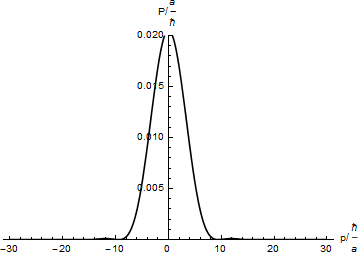
\includegraphics[scale=0.4]{fig/square-well-p.png}
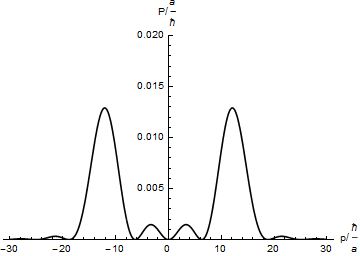
\includegraphics[scale=0.4]{fig/square-well-p-4.png}
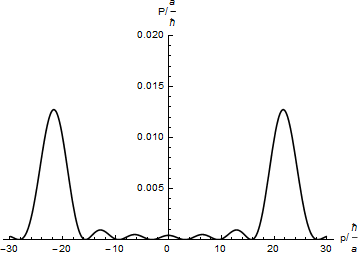
\includegraphics[scale=0.4]{fig/square-well-p-7.png}
\caption{粒子在方势阱里的动量分布}
\label{fig-square-well-p}
\end{figure}

算符在不同的表象下也有不同的样子。动量表象下的动量算符$\hat{p}$就是$p$,而位置算符$\hat{x}=\rmi \hbar \ppp$(注意这里没有负号,推导过程和刚才差不多)。想要在动量表象下计算平均位置,仍然可以对$\hat{x}$“计算平均值”:$\overline{x}=\int_{-\infty}^{\infty} \phi^* \hat{x} \phi \opd p$。

刚才推导位置表象下的动量算符用到了薛定谔方程。如果不知道薛定谔方程,利用傅立叶变换也可以推导:
\begin{align*}
\overline{p}&=\int_{-\infty}^{\infty} \phi^* p \phi \opd p \\
&=\frac{1}{\sqrt{2 \pi \hbar}} \int_{-\infty}^{\infty} \int_{-\infty}^{\infty} \psi^* \rme^{\frac{\rmi}{\hbar} p x} \opd x p \phi \opd p \\
&=\frac{1}{\sqrt{2 \pi \hbar}} \int_{-\infty}^{\infty} \int_{-\infty}^{\infty} \psi^* (-\rmi \hbar \ppx) \rme^{\frac{\rmi}{\hbar} p x} \opd x \phi \opd p \\
&=\int_{-\infty}^{\infty} \psi^* (-\rmi \hbar \ppx) \frac{1}{\sqrt{2 \pi \hbar}} \int_{-\infty}^{\infty} \phi \rme^{\frac{\rmi}{\hbar} p x} \opd p \opd x \\
&=\int_{-\infty}^{\infty} \psi^* (-\rmi \hbar \ppx) \psi \opd x
\end{align*}

在简谐波的表达式$\rme^{\rmi(k x-\omega t)}$中,位置和时间看起来是对称的(相差一个负号),动量和能量也是对称的。既然$\hat{p}=-\rmi \hbar \ppx$,那么$\hat{E}=\rmi \hbar \ppt$(相差一个负号),这就是薛定谔方程。

\chapter{波动光学}
\section{光波;光屏上的波函数}
在波动光学中,几束光射到同一个地方,光强不是简单的相加,而是光波的叠加,可能增强也可能减弱。(这一章里光强指的是能量通量密度,也就是单位时间、单位面积通过的能量,而眼睛感受到的光强测量起来更加复杂)

三维空间中的一个光源发出球面电磁波,波函数$\psi(r,t)=\frac{A_0}{r} \rme^{\rmi(k r-\omega t)}$,电磁场的每个分量都可以这样表示。(啊。。这不是量子力学里的波函数,如果是机械波的话$\psi$就是某个点在某个时刻的位移,电磁波的话就叫波函数好了)

跟前面一样,为了加减的运算方便,把它表示成复指数,但是乘除之前要先取实部。$\frac{A_0}{r}$是与光源距离为$r$的某个点上波的振幅,$\rme^{\rmi(k r-\omega t)}$则是相位。$A_0$表示光源的强度,同一个光源的$A_0$是相同的,这一章里先不管它。而且只考虑同一时刻的波,因此也不管$\rme^{-\rmi \omega t}$。$k=\frac{2 \pi}{\lambda}$,$\lambda$是波长。在同一时刻,距离每增加$\lambda$,相位就增加$2 \pi$。

振幅与$r$成反比,而光强是振幅的平方,与$r^2$成反比,这样才能保证任何一个球面上的能量通量$\Phi=(\frac{A_0}{r})^2 \cdot 4 \pi r^2$与$r$无关,能量是守恒的。

如图\ref{fig-wave-amp},在空间中有一个光屏和主光轴,交点为$O$。光源$S$在主光轴上,到光屏的距离为$z$,光屏上一点$P$到$O$的距离为$x$(以后还会把光屏看作$x-y$平面),那么$r=\sqrt{z^2+x^2}$。
\begin{figure}[htb]
\centering
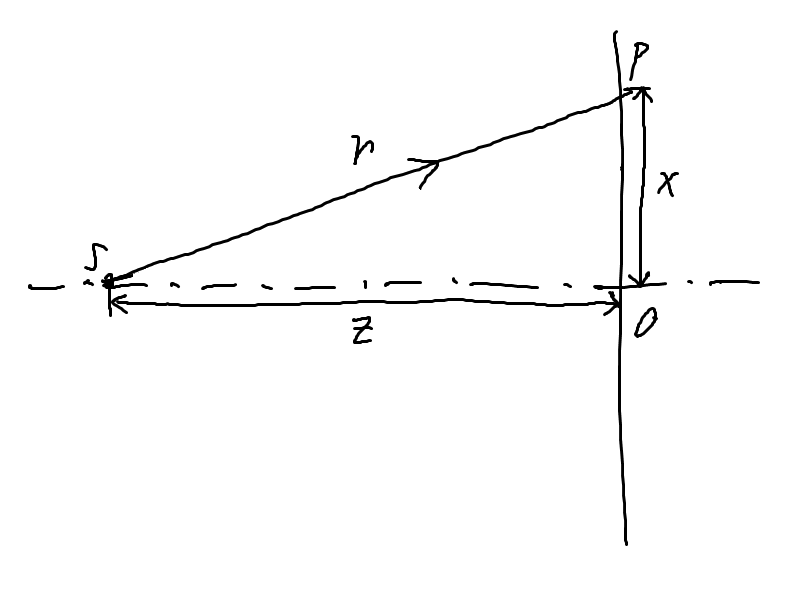
\includegraphics[width=0.33\linewidth]{fig/wave-amp.png}
\caption{传说主光轴要画成点划线但是手画很麻烦}
\label{fig-wave-amp}
\end{figure}

接下来要做一个近似:当$x \ll z$时,$r=z (1+\frac{x^2}{2 z^2})$,这个条件称为傍轴条件,因为光射到的位置离主光轴很近。这时振幅$\frac{A_0}{r}=\frac{A_0}{z (1+\frac{x^2}{2 z^2})}=\frac{A_0}{z}(1-\frac{x^2}{2 z^2})$,忽略高阶项,就是$\frac{A_0}{z}$。

而相位$\rme^{\rmi k r}=\rme^{\rmi k z} \rme^{\rmi k \frac{x^2}{2 z}}$。第一项$\rme^{\rmi k z}$与$x$无关,可以并到振幅里面去。然而$\lambda$很小,$k$很大,即使$x$有一点点变化,第二项$\rme^{\rmi k \frac{x^2}{2 z}}$也有很大的变化,不能再对它做近似。

(非要作近似也可以,当$\frac{x^2}{\lambda z} \ll 1$时,球面波就被近似成了平面波,整个光屏上的相位是一样的。这种情况称为远场条件)

如果光源不在主光轴上,到主光轴的距离为$x_0$(在同一个平面上),可以把$x$改成$x-x_0$。最后光屏上的波函数是
\begin{equation*}
\psi(x,x_0)=A \rme^{\rmi k \frac{(x-x_0)^2}{2 z}}
\end{equation*}

如果有几束光射到同一个地方,它们的波函数可以相加,光强则是波函数之和的模长的平方,跟量子力学当中波函数与概率的关系差不多。

(要求这几束光是相干的,也就是它们的振动方式一样,这又是一个复杂的问题。现在我们只要知道,同一个光源发出的光是相干的,被双缝分成两份之后也是)
\section{双缝干涉}
高中物理课本讲过双缝干涉,可以用小角近似的方法算条纹间距(虽然有些版本的课本连公式都没有讲)。这里用波函数的方法再算一遍。

设两条缝在$\pm x_0$处,光屏上的波函数$\psi=A (\rme^{\rmi k \frac{(x-x_0)^2}{2 z}}+\rme^{\rmi k \frac{(x+x_0)^2}{2 z}})$,光强则是
\begin{align*}
F&=\psi \psi^* \\
&=A^2 (\rme^{\rmi k \frac{(x-x_0)^2}{2 z}}+\rme^{\rmi k \frac{(x+x_0)^2}{2 z}})(\rme^{-\rmi k \frac{(x-x_0)^2}{2 z}}+\rme^{-\rmi k \frac{(x+x_0)^2}{2 z}}) \\
&=A^2 (2+\rme^{\rmi k B}+\rme^{-\rmi k B}) \\
&=A^2 (2+2 \cos k B) \\
&=4 A^2 \cos^2 \frac{k B}{2} \\
\text{其中}B&=\frac{(x+x_0)^2-(x-x_0)^2}{2 z} \\
&=\frac{2 x_0 x}{z} \\
F&=4 A^2 \cos^2 \frac{k x_0}{z} x \\
&=4 A^2 \cos^2 2 \pi \frac{x_0}{\lambda z} x
\end{align*}

所以光强$F$是余弦的平方,周期为$\frac{\lambda z}{2 x_0}$。而双缝的间距$d=2 x_0$,所以周期为$\frac{\lambda z}{d}$。不但能算出两个最亮处或者最暗处的间距,还能算出其他地方的光强。

要强调的是,这些结果只有在傍轴近似下成立,所以只有双缝正对着的一小块地方能看到清晰的条纹,我们平常看到一大排条纹的图片一般是放大过的。
\section{无穷远处的波函数}
距离为$z$的光屏上有波函数,无穷远处也有波函数。如图\ref{fig-wave-amp-inf}左侧,光源是一个一维的物体,有一根主光轴与它垂直,交点$S$的坐标为$0$。物体向无穷远处的各个方向射出平行光(图中只画了一个方向),与主光轴的夹角为$\theta$。这一章里$\theta \ll 1$。
\begin{figure}[htb]
\centering
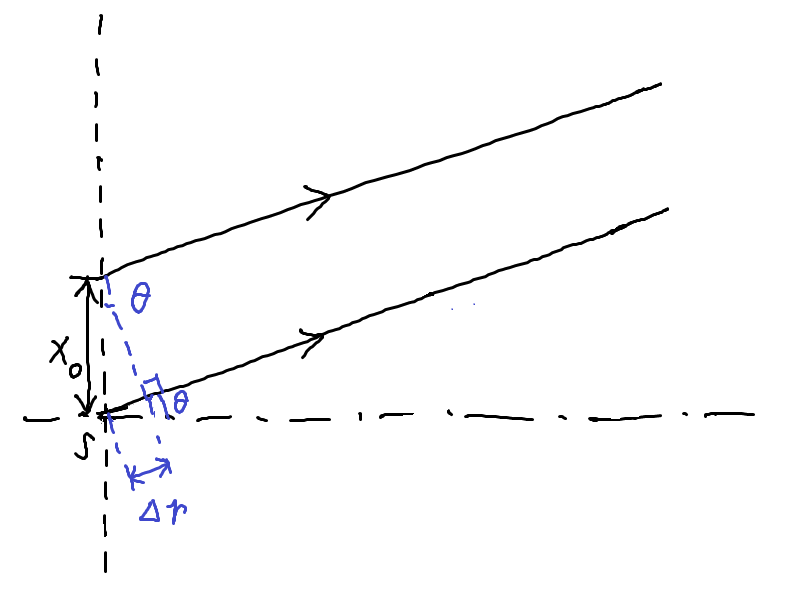
\includegraphics[width=0.33\linewidth]{fig/wave-amp-inf.png}
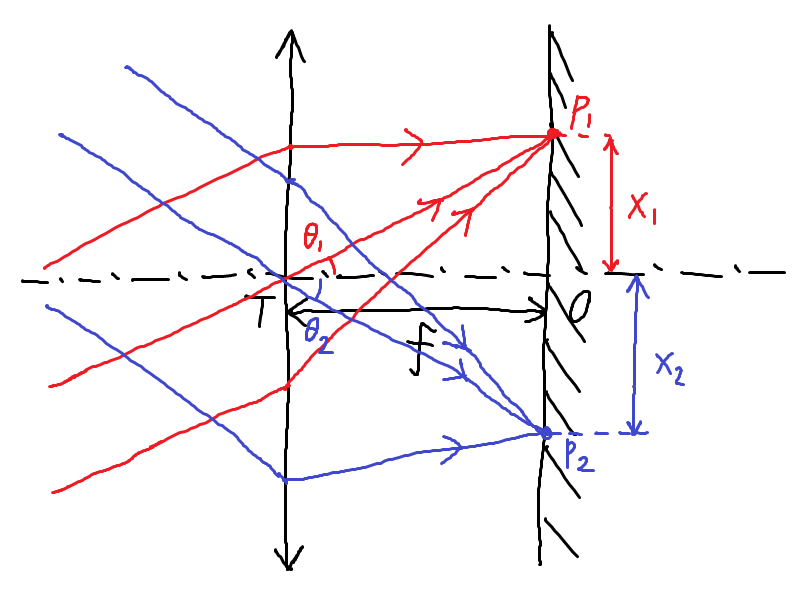
\includegraphics[width=0.33\linewidth]{fig/conv-lens.png}
\caption{射向无穷远,再用凸透镜聚焦}
\label{fig-wave-amp-inf}
\end{figure}

(注意这里的所有结论都在$\theta \ll 1$时才成立,图中为了清楚把$\theta$画得比较大)

物体上可以有很多个点发光,如果一个点与$S$的距离为$x_0$,它发出的光比$S$处的光少走光程$\delta r=x_0 \sin \theta=x_0 \theta$,相位差为$\rme^{-\rmi k x_0 \theta}$。

用凸透镜可以把一束射向无穷远的平行光聚焦到一个点上。如图\ref{fig-wave-amp-inf}右侧,角度为$\theta$的平行光聚焦到点$P$,位置$x=f \sin \theta=f \theta$,$f$是透镜的焦距。把射到$P$点的每条光线的波函数加起来,就是$P$点上的波函数,也代表无穷远处$\theta$方向的波函数。

(这里的平行光是无限宽的,透镜也是无限大的,所以上下移动平行光不会改变聚焦的位置,只有改变平行光的方向才能改变聚焦的位置。无限宽的平行光和傍轴近似是矛盾的,但是这里就这么算吧,反正是理想模型。另外,每条光线通过透镜的光程都是相同的,这个问题也不讲了)

高中做双缝干涉的实验时一般不会在屏前面用凸透镜成像。如果用凸透镜成像,观察无穷远处的光强,结果会怎么样呢?
\begin{align*}
\psi&=A(\rme^{-\rmi k x_0 \theta}+\rme^{\rmi k x_0 \theta}) \\
&=2 A \cos k x_0 \theta \\
F&=\psi \psi^* \\
&=4 A^2 \cos^2 k x_0 \theta \\
&=4 A^2 \cos^2 \frac{k x_0}{z} x \\
&=4 A^2 \cos^2 2 \pi \frac{x_0}{\lambda z} x
\end{align*}

在我们的近似下,结果和有限远处一样,但是计算会简便一些。接下来的问题严格来说都要用凸透镜来聚焦平行光,但是实验当中经常会直接用屏来成像,只要屏够远,误差不会很大。
\section{单缝衍射}
如图\ref{fig-silt-diff},一条狭缝宽度为$a$,里面的每个点都射出光线。我们一般把有限个光源的叠加叫干涉,而把无限个光源的叠加叫衍射。
\begin{figure}[htb]
\centering
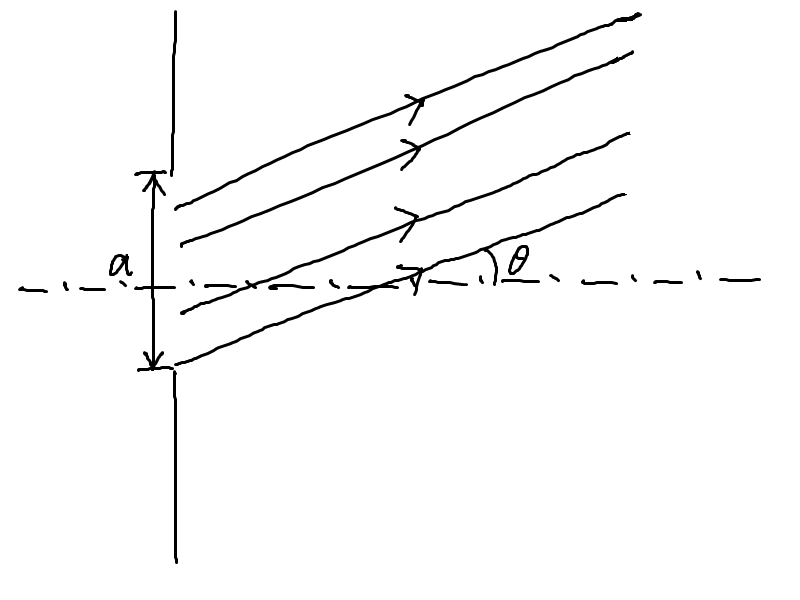
\includegraphics[width=0.33\linewidth]{fig/silt-diff.png}
\caption{这条缝其实是很细的}
\label{fig-silt-diff}
\end{figure}

计算波函数需要积分:
\begin{align*}
\psi&=\int_{-\frac{a}{2}}^{\frac{a}{2}} A \rme^{-\rmi k x_0 \theta} \opd x_0 \\
&=\frac{\rmi A}{k} (\rme^{-\rmi \frac{k a \theta}{2}}-\rme^{\rmi \frac{k a \theta}{2}}) \\
&=2 \frac{A}{k} \sin \frac{k a \theta}{2}
\end{align*}

设$\alpha=\frac{k a \theta}{2}=\frac{\pi a \theta}{\lambda}$,那么$\psi=A \frac{\sin \alpha}{\alpha}$。$\frac{\sin x}{x}$是一个在光学中经常用到的函数,有些地方叫作\emph{读数函数}或者$\sinc x$。

光强则是$F=\psi^2=A^2 (\frac{\sin \alpha}{\alpha})^2$,如图\ref{fig-silt-diff-plot},中间有一个明显的峰,称为零级峰,旁边还有一级峰,二级峰等等,但是在实验中不容易看到。从图像下面的面积可以看出,零级峰占了总能量的90\%。
\begin{figure}[htb]
\centering
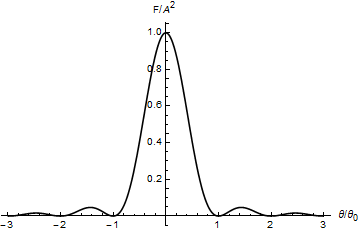
\includegraphics[width=0.33\linewidth]{fig/silt-diff-plot.png}
\caption{迷之凸起}
\label{fig-silt-diff-plot}
\end{figure}

$\alpha$是一个无量纲的数。$\theta=\frac{\lambda}{a}$时,$\alpha=\pi$,$F=0$,所以它是零级峰的半角宽度。注意它是一个角度,零级峰的宽度还要取决于聚焦用的透镜焦距。增大$\lambda$或者减小$a$,条纹就会变宽。

一般认为缝宽$a$是光波长$\lambda$的$\frac{1}{5}$到$5$倍时,衍射是比较明显的。可见光的波长是几百纳米,而实验用的缝宽一般是几微米。
\section{双缝干涉中的衍射}
刚才把双缝干涉的每条缝都当作一个点,实际上它们发出的光也会衍射,有什么影响呢?

一条缝发出的波函数就是$\psi_1=A \frac{\sin \alpha}{\alpha}$,另一条缝与它的距离是$d$,可以直接乘上一个相位差$\rme^{-\rmi k d \theta}$。两条缝的波函数之和是
\begin{align*}
\psi&=\psi_1 (1+\rme^{-\rmi k d \theta}) \\
&=2 \psi_1 \cos \frac{k d \theta}{2} \rme^{-\rmi \frac{k d \theta}{2}} \\
&=2 \rme^{-\rmi \frac{k d \theta}{2}} A \frac{\sin \alpha}{\alpha} \cos \frac{k d \theta}{2}
\end{align*}

$2 \rme^{-\rmi \frac{k d \theta}{2}} A$是常数,这里不用考虑。设$\beta=\frac{k d \theta}{2}$,那么$F=\psi^2=(\frac{\sin \alpha}{\alpha} \cos  \beta)^2$,也就是双缝干涉的光强乘上了一个单缝衍射的光强。

$\frac{d}{a}=10$时,$F$的图像如图\ref{fig-silt-diff-plot-2}。双缝干涉会产生比较密的峰$(\cos \beta)^2$,而单缝衍射的因子$(\frac{\sin \alpha}{\alpha})^2$让远处的峰高度降低。
\begin{figure}[htb]
\centering
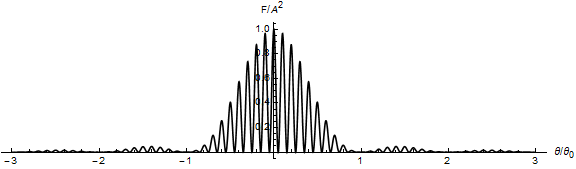
\includegraphics[width=0.33\linewidth]{fig/silt-diff-plot-2.png}
\caption{峰里有峰}
\label{fig-silt-diff-plot-2}
\end{figure}

为了清楚,画图时的$\frac{d}{a}$比较小。实验中$a$一般是几微米,而$d$是几毫米,$\frac{d}{a}=1000$,单缝衍射的零级峰里可以放下更多双缝干涉的峰。再加上小角近似的限制,实验中观察到的干涉条纹只有最中间那几条,而缝宽对它们几乎没有影响。
\section{形状因子与结构因子}
现在双缝干涉的波函数可以分成两部分:形状因子$\psi_f=\frac{\sin \alpha}{\alpha}$表示每根缝的形状,结构因子$\psi_s=\cos \beta$表示两根缝的位置关系,而$\psi=\psi_f \psi_s$。如果把两根缝换成圆孔或者其他东西,只要改变$\psi_f$;如果增加更多的缝,或者改变缝的相对位置和相对光强,只要改变$\psi_s$。

举个栗子:如果有三根缝分别在位置$0,x_1,x_2$,相对光强分别为$1,2,3$,可以直接写出$\psi=\frac{\sin \alpha}{\alpha}(1+2 \rme^{-\rmi k x_1 \theta}+3 \rme^{-\rmi k x_2 \theta})$,形状因子还是单缝,结构因子则是$\psi_s=1+2 \rme^{-\rmi k x_1 \theta}+3 \rme^{-\rmi k x_2 \theta}$。

我们知道X射线衍射可以分辨晶体的结构,而晶体是由许多相同的分子排列成的,衍射图案可以反映出分子形状和排列方式,把衍射图案分成形状因子与结构因子就是把两者分开。
\section{光栅}
把许多狭缝排在一起就变成了光栅(读作shān)。设光栅上总共有$N$条缝,每条缝的宽度为$a$,缝与缝之间不透光部分的宽度为$b$。如果把一条缝平移$d=a+b$,就与另一条缝重合,所以我们用$d$表示缝的距离(而不是$b$)。一般的光栅每毫米有几百条缝。

光栅的形状因子仍然是$\frac{\sin \alpha}{\alpha}$,而结构因子是等比数列:
\begin{align*}
\psi_s&=1+\rme^{-\rmi k d \theta}+\rme^{-2 \rmi k d \theta}+\dots+\rme^{-(N-1) \rmi k d \theta} \\
&=\frac{1-\rme^{-\rmi N k d \theta}}{1-\rme^{-\rmi k d \theta}} \\
&=\frac{\rme^{-\rmi N \frac{k d \theta}{2}} (\rme^{\rmi N \frac{k d \theta}{2}}-\rme^{-\rmi N \frac{k d \theta}{2}})}{\rme^{-\rmi \frac{k d \theta}{2}} (\rme^{\rmi \frac{k d \theta}{2}}-\rme^{-\rmi \frac{k d \theta}{2}})} \\
&=\rme^{-\rmi (N-1) \frac{k d \theta}{2}} \frac{\sin N \beta}{\sin \beta}
\end{align*}

其中$\beta$仍然是$\frac{k d \theta}{2}$。$N=2$时,就是上面的双缝干涉。

光强$F=\psi \psi^*=(\frac{\sin \alpha}{\alpha})^2 (\frac{\sin N \beta}{\sin \beta})^2$。$\frac{d}{a}=10,N=2,4,6,8$时,$F$如图\ref{fig-grate}。可以看出,$N$越大,条纹越尖锐。
\begin{figure}[htb]
\centering
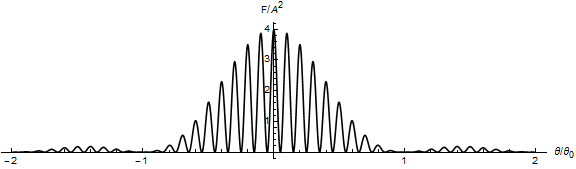
\includegraphics[width=0.33\linewidth]{fig/grate-2.png}
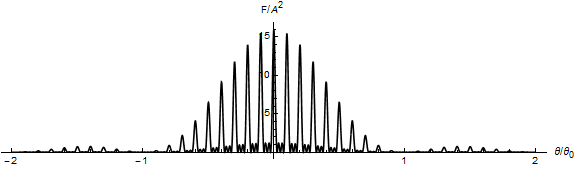
\includegraphics[width=0.33\linewidth]{fig/grate-4.png} \\
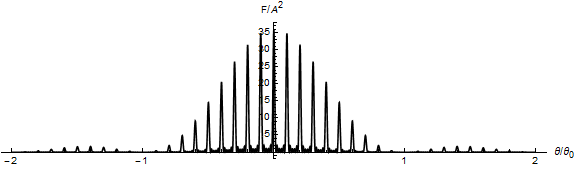
\includegraphics[width=0.33\linewidth]{fig/grate-6.png}
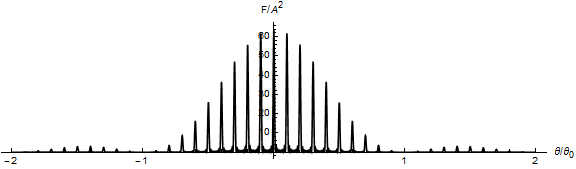
\includegraphics[width=0.33\linewidth]{fig/grate-8.png}
\caption{如果$N$和$\frac{d}{a}$很大的话图片根本看不清}
\label{fig-grate}
\end{figure}
\section{衍射与傅立叶变换}
(这一节也要看过后面的傅立叶变换才能看)

一个一维的物体可以看成亮度关于位置的函数$A(x_0)$。它可以有些地方发光,有些地方不发光,发光的地方亮度也可以不一样。无穷远处的波函数可以表示成积分:
\begin{equation*}
\psi(\theta)=\int_{-\infty}^{\infty} A(x_0) \rme^{-\rmi k x_0 \theta} \opd x_0
\end{equation*}

而傅立叶变换的公式是:
\begin{align*}
g(k)&=\mathscr{F}_{x \rightarrow k} f(x)=\frac{1}{\sqrt{2 \pi}} \int_{-\infty}^{\infty} f(x) \rme^{-\rmi k x} \opd x &
f(x)&=\mathscr{F}^{-1}_{x \rightarrow k} g(k)=\frac{1}{\sqrt{2 \pi}} \int_{-\infty}^{\infty} g(k) \rme^{\rmi k x} \opd k
\end{align*}

可以发现,$\psi(\theta)=\sqrt{2 \pi} \mathscr{F}_{x_0 \rightarrow k \theta} A(x_0)$。在傍轴、无穷远的条件下,衍射就是一个傅立叶变换。在电脑还不够先进的时候,确实有人做出了这样的光学装置来实现傅立叶变换。

如果忽略双缝的缝宽,它就是两个$\delta$函数,变换之后是余弦函数。单缝是一个方形窗,变换之后是$\frac{\sin x}{x}$类型的函数。

\chapter{量纲分析与原子物理}
\section{量纲}
量纲是一种和单位差不多的东西,每个物理量有它的单位,也有它的量纲。我们用方括号大写字母表示量纲(虽然打草稿的时候肯定不会这么写),常用的量纲有长度$[L]$,质量$[M]$,时间$[T]$,电流$[I]$和温度$[\Theta]$。($\Theta$的读音是theta,而拉丁文的“温度”是thermo)

比如长度$l$这个物理量的量纲是$[L]$。不管它的单位是米、厘米还是英寸,它的量纲都是$[L]$。

再比如公式$F=m a$,$m$的量纲是$[M]$,$a$的量纲是$[L] [T]^{-2}$,所以$F$的量纲是$[L] [M] [T]^{-2}$。一个等式两边的量纲必须相等,做完题目之后记得检查这一点。同一个矩阵的元素量纲必须相同,否则矩阵乘法就没有意义。

下面是一些常见物理量的量纲:

\begin{tabular}{lrlr}
能量$E$与力矩$M$ & $[L]^2 [M] [T]^{-2}$ & 角动量$L$ & $[L]^2 [M] [T]^{-1}$ \\
引力常量$G$ & $[L]^3 [M] [T]^{-2}$ & 静电力常量$k$ & $[L]^3 [M] [T]^{-4} [I]^{-2}$ \\
电压$U$ & $[L]^2 [M] [T]^{-3} [I]^{-1}$ & 电阻$R$ & $[L]^2 [M] [T]^{-3} [I]^{-2}$ \\
电场强度$E$ & $[L] [M] [T]^{-3} [I]^{-1}$ & 磁感应强度$B$ & $[M] [T]^{-2} [I]^{-1}$ \\
真空介电常量$\epsilon_0$ & $[L]^{-3} [M]^{-1} [T]^4 [I]^2$ & 真空磁导率$\mu_0$ & $[L] [M] [T]^{-2} [I]^{-2}$ \\
\end{tabular}

【练习】用你熟悉的公式把这些东西推导一遍。现在不用背下来,用得多了就背下来了。

如果你现在不能理解量纲是什么,理解成单位也没问题。
\section{量纲分析}
考虑这样一个问题:在太空中放一个水球,然后戳它一下,由于表面张力作用,它会发生振动,求振动频率。

首先猜一猜频率可能与哪些物理量有关,这一步需要传说中的“物理直觉”。我们先猜频率$f$与球的半径$r$、水的密度$\rho$、水的表面张力系数$\sigma$有关。

(介绍一下表面张力系数:液体与固体或者气体的分界面会产生一个势能$E=\sigma S$,叫作表面能。$S$是分界面的面积,液体会尽量减小$S$来使能量最低。)

$f$的量纲是$[T]^{-1}$,$r$的量纲是$[L]$,$\rho$的量纲是$[L]^{-3} [M]$,$\sigma$的量纲是$[M] [T]^{-2}$。

设$f=A r^a \rho^b \sigma^c$,$A$是一个无量纲的系数。等式两边的量纲必须相等,因此对$[L],[M],[T]$分别列出方程:
\begin{equation*}
\begin{cases}
a-3b=0 \\
b+c=0 \\
-2c=-1
\end{cases}
\end{equation*}

解得$a=-\frac{3}{2},b=-\frac{1}{2},c=\frac{1}{2}$,也就是说$f=A \sqrt{\frac{\sigma}{\rho r^3}}$。量纲分析并不能确定$A$,但是有些问题中$A$并不重要,只要知道$r,\rho,\sigma$变化时$f$大致的变化情况就行了。(想想之前讲的复杂度理论)事实上,用一些流体力学方法可以算出$A$的最小值为$2\sqrt{2}$。

我们要相信物理学中的每个系数都是有它出现的原因的,比如$2$通常是$x^2$求导留下的,$\pi$通常在画了一个圆或者球之后出现,至于$\sqrt{57 \pi}$这样奇怪的系数就没有道理出现在基本的公式里。

如果单位制合适,$A$的大小不会跟$1$相差太多。比如你用毫米量一根杆子的长度是$1000$多,只要改用米来量就和$1$差不多了。

现在回过头一看:$\rho r^3$和质量$m$的量纲是相同的。如果一开始猜$f$与$m,\sigma$有关,那么这道题就秒杀了。量纲分析能否成功,以及过程有多复杂会受一开始猜的参量影响,如果参量猜得太多,方程数量就不够;如果参量猜得太少,就凑不出需要的量纲。

再来看一个复(zhuang)杂(bi)的例子:把两块无限大的薄导体板放在真空中,根据量子电动力学,两块板之间会出现一些电磁场的涨落,所以它们会相互吸引,这个效应称为\emph{卡西米尔效应}。我们来求吸引力造成的压强。

卧槽这是什么鬼!但是我们要相信,给我们做的题目总是有办法做出来的。因为板是无限大的,所以它们的质量和面积都没有意义。(两块板之间的吸引力大小也没有意义,但是单位面积的吸引力、也就是压强是有意义的)而且板是薄的,也就是说它们的厚度没有意义。但是两块板的间距$d$可以当作一个参量。

为了凑出压强的量纲,还要用一些物理常量:这道题与量子有关,所以可能需要普朗克常量$h$;还与电磁场有关,所以可能需要光速$c$和真空介电常量$\epsilon_0$。

(做这样的题目需要一些物理常识。如果题目与相对论有关,可能需要光速$c$;如果题目与万有引力或者广义相对论有关,可能需要引力常量$G$;如果题目与分子运动有关,可能需要玻尔兹曼常量$k$。这里的吸引力并不是万有引力)

设压强$p=A d^\alpha h^\beta c^\gamma \epsilon_0^\delta$。($c$和$d$都被用掉了好悲伤)

对$[L],[M],[T],[I]$分别列出方程:($p$的量纲是$[L]^{-1} [M] [T]^{-2}$,$h$的量纲是$[L]^2 [M] [T]^{-1}$)
\begin{equation*}
\begin{cases}
\alpha+2\beta+\gamma-3\delta=-1 \\
\beta-\delta=1 \\
-\beta-\gamma+4\delta=-2 \\
\delta=0
\end{cases}
\end{equation*}

诶我写到这里才想起来$\delta=0$,所以其实我们并不需要$\epsilon_0$。解得$\alpha=-4,\beta=1,\gamma=1$,所以$p=A \frac{h c}{d^4}$。
\section{无量纲数}
只有量纲相同的东西才能比较大小,比如你可以说一根棍子比另一根棍子长,但是不能说一根棍子的长度比另一根棍子的重量大。

事实上,比较物理量大小的本质是比较无量纲数的大小,比如一根棍子的长度$l_1$比另一根棍子的长度$l_2$大,就是说无量纲数$\frac{l_1}{l_2}>1$。不管用米、厘米还是英寸来量它们的长度,都是第一根棍子比较长。无量纲数可以描述一个物理系统的性质,而与单位制无关。再比如阻尼振动是欠阻尼、临界阻尼还是过阻尼,就是由无量纲数$\frac{\omega_0}{\beta}$决定的。

$\sin x,\exp x$等函数的自变量必须是无量纲数,比如$\sin \omega t$,$\exp -\frac{\hbar \omega}{k T}$。角度也是无量纲的,比如角速度$\omega$的单位是$\unit{rad/s}$,量纲是$[T]^{-1}$。

在高考中我们经常遇到$t=\sqrt{\frac{2 h}{g}}$,$v=\sqrt{2 g h}$等等,在打草稿的时候可以设$t_0=\sqrt{\frac{h}{g}}$,$v_0=\sqrt{g h}$,那么$t=\sqrt{2} t_0$,$v=\sqrt{2} v_0$。计算的时候只要算前面的系数就行了,后面的字母可以根据量纲补上。比如$x=v t$,那么$x$的系数是$2$,后面是$h$。$a=\frac{v}{t}$,那么$a$的系数是$1$,后面是$g$。更复杂的例子等要用的时候再讲。
\section{精细结构常数;秒杀原子物理题}
现在来看看玻尔的氢原子模型。假设原子核与电子之间的力满足库仑定律$F=\frac{1}{4 \pi \epsilon_0} \frac{e^2}{r^2}$,电子的运动满足牛顿第二定律$F=m_e \frac{v^2}{r}$,以及量子化条件$m_e v r =n \hbar (n=1,2,3,\dots)$。

($\hbar=\frac{h}{2 \pi}=1.05 \times 10^{-34} \unit{J \cdot s}$,叫作约化普朗克常量,读作h bar。在原子物理中,频率$f$和角速度$\omega$相差一个系数$2 \pi$,所以有时候用$\hbar$比$h$更方便)

解得电子轨道半径$r=\frac{4 \pi \epsilon_0 \hbar^2 n^2}{e^2 m_e}$,速度$v=\frac{e^2}{4 \pi \epsilon_0 \hbar n}$,还可以计算出能量$E=\frac{1}{2} m_e v^2-\frac{1}{4 \pi \epsilon_0} \frac{e^2}{r}=-\frac{e^4 m_e}{2 (4 \pi \epsilon_0)^2 \hbar^2 n^2}$,代入数值可以算出我们熟悉的$E=-\frac{13.6}{n^2} \unit{eV}$。

(这些物理量的数值在卡西欧计算器上都有,但是卡西欧直接算$e^4 m_e$会因为数值太小而报错,需要拆成两部分来算)

【练习】用能量最低原理和量子化条件把这些东西推导一遍。

有没有简便一点的计算方法呢?我们定义一个无量纲数:精细结构常数$\alpha=\frac{e^2}{4 \pi \epsilon_0 \hbar c} \approx \frac{1}{137}$。这是用$e,\epsilon_0,\hbar,c$能凑出的最简单(指数是整数且最小)的无量纲数。注意我们并没有选电子质量$m_e$,因为它是电子的特性;而$e$不仅是电子电量,而是电荷的基本单位,它的地位比$m_e$更基本。

$\alpha$里面有一个系数$\frac{1}{4 \pi}$,因为我们经常需要在一个电荷周围画一个球面然后算它的面积,所以为了方便就把$\frac{1}{4 \pi}$放进去了。

现在我们发现$v=\frac{\alpha}{n} c$,$r=(\frac{\alpha}{n})^{-1} \frac{\hbar}{m_e c}$,$E=-\frac{1}{2} m_e v^2=-\frac{1}{2} (\frac{\alpha}{n})^2 m_e c^2$。这样一来这些结果的物理意义就比较清楚,而且比较容易背下来。

$m_e v r =n \hbar$里$n$和$\hbar$是相乘的,所以$\alpha$肯定会与$n$相除。$\frac{\hbar}{m_e c}$是$\hbar,m_e,c$能凑出的最简单的无量纲数,它叫作电子的约化康普顿波长,讲相对论的时候说不定还会碰到它。

【练习】如果原子核的电量为$+Z e$,核外只有一个电子,求电子的轨道半径和能量,想一想要对$\alpha$作怎样的修改。
\section{数量级估计}
在热学中我们知道单原子气体分子热运动的平均动能$E_k=\frac{1}{2} m v^2=\frac{3}{2} k T$,$v=\sqrt{\frac{3 k T}{m}}=\sqrt{\frac{3 R T}{\mu}}$。如果把系数当成$1$,我们可以认为$v_T=\sqrt{\frac{R T}{\mu}}$就是分子热运动大致的速度,多原子气体也差不了多少。温度越高,分子质量越小,热运动就越剧烈。空气的$\mu=29 \unit{g/mol}$,我们认为常温是$T=300 \unit{K}$,那么$v_T=3 \times 10^2 \unit{m/s}$。氢气则有$v_T=1 \times 10^3 \unit{m/s}$。(这种估算一般只需要一位有效数字,甚至只需要数量级)

在量子力学中我们又知道德布罗意波长$\lambda=\frac{h}{m v}=\frac{h N_A}{\mu v}$。如果$v=v_T$,我们把这个波长叫作分子的热波长$\lambda_T$,也就是热运动引起的位置不确定程度。空气在常温下$\lambda_T=5 \times 10^{-11} \unit{m}$。

而在经典的热学中,空气满足$p V=n R T$,设两个空气分子的距离为$d$,那么$V=n N_A d^3$,所以$d=(\frac{R T}{N_A p})^{\frac{1}{3}}=3 \times 10^{-9} \unit{m}$。$d \gg \lambda_T$,所以分子之间的量子效应是不显著的。如果温度降低,$\lambda_T$增大,$d$减小,$\lambda_T$接近甚至超过$d$,量子效应就会很显著,这就是传说中的凝聚态物理学研究的东西。

$k T$具有能量的量纲,估算分子的能量时,可以认为温度为$T$时能量就是$k T$。

比如我们要估算核聚变的温度,可以认为核聚变就是把两个质子从无穷远处移到碰到一起为止,这个过程中电势能升高,忽略其他相互作用。但是两个质子之间的距离如果为$0$,电势能就会变得无穷大,什么叫碰到一起呢?可以认为它们的距离是原子核的大小$d=10^{-15} \unit{m}$。现在可以列出$\frac{e^2}{4 \pi \epsilon_0 d}=k T$,所以$T=\frac{e^2}{4 \pi \epsilon_0 d k}=10^{10} \unit{K}$。($k T$是一个还是两个质子的动能就不管了,数量级没有区别)

为了做这样的题目,平常可以留意一些东西的大致数值,比如水的折射率是1.33(稀溶液不会差太多),$1 \unit{g}$ TNT爆炸的能量是$4 \times 10^3 \unit{J}$,地磁场的强度是$5 \times 10^{-5} \unit{T}$,铜的电阻率是$2 \times 10^{-8} \unit{\Omega \cdot m}$,樱花瓣飘落的速度是每秒$5$厘米等等,说不定哪天可以用上。(建议背一下地球、月球、太阳、火星的半径、轨道半径、质量、温度)
\section{国际单位制}
(这些内容可以作为常识了解一下)

国际单位制中有七个基本物理量:长度、质量、时间、电流、温度、发光强度、物质的量。它们的基本单位分别是米、千克、秒、安培、开尔文、坎德拉、摩尔。

很久以前测量电流比电量更方便,所以基本物理量是电流而不是电量。发光强度表示特定方向上眼睛感受到的光的强度,它与光携带的能量并不成正比,而要通过复杂的关系来换算,它的量纲也比较特殊。物质的量专门有一个量纲,但是不太常用。

接下来讲这些基本单位的定义:

铯-133原子发出的某种电磁波的周期的$9192631770$倍为$1$秒。(当然这些数字不用记得很仔细)

光在真空中、在$1/299792458$秒内走过的长度为$1$米。

国际千克原器的质量为$1$千克。(国际千克原器是保存在巴黎的一个金属块,是不是很扯蛋)

真空中有两根无限长、无限细的平行直导线,相距$1$米,往里面通等大的电流,当它们受到每米$1$牛顿的安培力时,通的电流就是$1$安培。

开尔文现在的定义需要一些热力学知识,这里先不讲了。温度有一个特殊之处:其他单位只需要定义相对值,而不需要定义绝对值,比如$1$米的长度需要我们定义,而$0$米并不需要我们定义。但是物理学当中存在一个最低温度——绝对零度,我们需要定义$0 \unit{K}$等于这个温度。以前的一段时间里是这样定义的:一个标准大气压下水的凝固点为273.15K,沸点为373.15K,这样既可以确定$0 \unit{K}$这一温度,又可以确定$1 \unit{K}$这一温度差。

0.012千克碳-12的原子数为1摩尔。

坎德拉的定义比较复杂,这里也不讲了。

近年来许多物理学家希望对上面这些定义作一些修改。特别是千克的定义,很大程度上是人为规定的。而安培的定义在实际操作中十分困难。

米的定义就比较好:先定义秒,再定义光速$c=299792458 \unit{m/s}$,就有了米的定义。物理学家希望用这种方式定义其他单位,比如定义普朗克常量$h=6.63 \times 10^{-34} \unit{m^2 \cdot kg \cdot s^{-1}}$,就有了千克的定义。当然三位有效数字是远远不够的,需要用精确的实验手段把$h$测到十几位有效数字,这样的定义才能被大家同意。类似地可以用元电荷$e$定义安培,用玻尔兹曼常量$k$定义开尔文。新的国际单位制有望在2018年被一帮开会的人通过。

顺便说一下,$c$是定义出来的精确值,$\mu_0=4 \pi \times 10^{-7} \unit{m \cdot kg \cdot s^{-2} \cdot A^{-2}}$也是,所以$\epsilon_0$是可以算出来的精确值。

\chapter{实验误差}
\section{误差与全微分}
我们做实验的时候一般是直接测量一些物理量,用它们算出另一些物理量。比如测得的物理量是$x,y$,算出的物理量$f$可以表示为$f(x,y)$。如果$x$的测量值与真实值相差$\Delta x$,而$y$是准确的,那么$f$与真实值相差$\Delta f=\frac{\partial f}{\partial x} \Delta x$。(这里仍然不管差分算符$\Delta$、微分算符$\opd$和偏微分算符$\partial$的区别)

如果$y$的测量值与真实值相差$\Delta y$,而$x$是准确的,那么$\Delta f=\frac{\partial f}{\partial y} \Delta y$。同时考虑$\Delta x$和$\Delta y$,那么$\Delta f$就是上面两种情况之和:$\Delta f=\frac{\partial f}{\partial x} \Delta x+\frac{\partial f}{\partial y} \Delta y$。

这其实就是对$f$求全微分:$\opd f=\frac{\partial f}{\partial x} \opd x+\frac{\partial f}{\partial y} \opd y$。

上面说的是知道$x$的测量值与真实值的差,计算$f$与真实值的差。但是$x$与真实值的差实际上是不知道的,$\Delta x$一般指的是最大误差。(它是一个大于$0$的量,专业一点叫作\emph{极限不确定度})

误差可以分为系统误差和偶然误差,系统误差永远向一边偏,偶然误差可以向两边偏。这里我们主要讨论偶然误差。

考虑最坏情况,$f$的误差$\Delta f=|\frac{\partial f}{\partial x}| \Delta x+|\frac{\partial f}{\partial y}| \Delta y$。其中$\frac{\partial f}{\partial x}$和$\frac{\partial f}{\partial y}$取绝对值,也就是说这两个量即使在公式里相互抵消,计算误差时也不能抵消。

举个栗子,如图\ref{fig-length-diff},我们用刻度尺测量一个长度$l$,两头的读数分别是$x_1$和$x_2$,那么$l=x_2-x_1$,但是$\Delta l=\Delta x_2+\Delta x_1$。
\begin{figure}[htb]
\centering
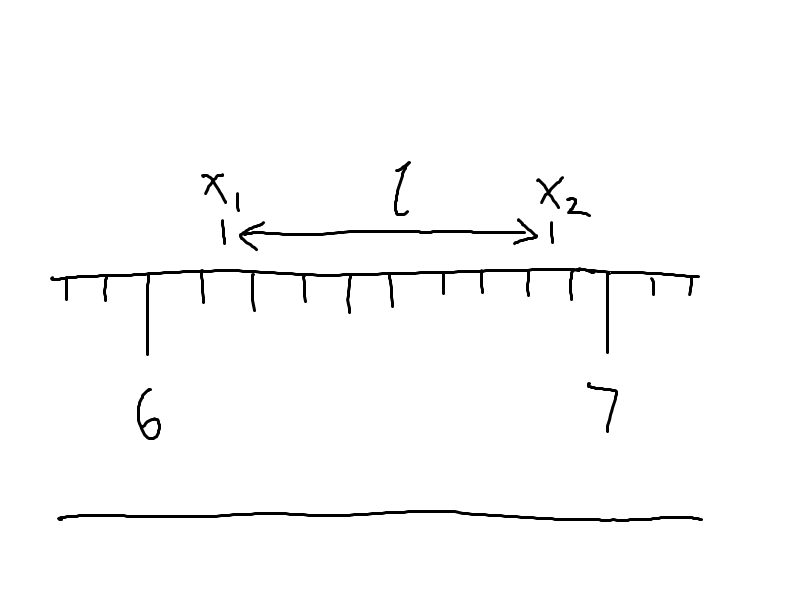
\includegraphics[width=0.33\linewidth]{fig/length-diff.png}
\caption{一把肥硕的尺子}
\label{fig-length-diff}
\end{figure}

再比如伏安法测电阻,$R=\frac{U}{I}$,$\Delta R=\frac{1}{I} \Delta U+\frac{U}{I^2} \Delta I$。

注意:用这种方法计算$f(x,y)$的误差,要求$x$与$y$无关。我们的物理课上发生过这么一件事:用打点计时器测加速度,有人用前半段纸带算一个加速度$a_1$,后半段纸带算一个加速度$a_2$,然后把$a_1$和$a_2$平均,结果发现误差比想象的大。事实上计算$a_1$和$a_2$用的一些点是相同的,$a_1$和$a_2$就是相关的,不能直接计算平均后的误差。

两个物理量是否相关有时候并不显然,需要通过实验来检验:测量多组$x$和$y$,看看它们之间有没有什么统计规律。(很多生物实验干的就是这样的事情)
\section{绝对误差与相对误差}
上面说的误差都是绝对误差,有时还会用到相对误差,比如$x$的相对误差为$|\frac{\Delta x}{x}|$。(严格来说分母应该是真实值,我们一般用测量值代替)

我们说的误差有时指绝对误差,有时指相对误差,要看具体情况。几个量加减的时候计算绝对误差比较方便,几个量乘除的时候计算相对误差比较方便。比如把上面伏安法测电阻的式子除以$R$得到$\frac{\Delta R}{R}=\frac{\Delta U}{U}+\frac{\Delta I}{I}$。

如果$x$是直接测量的量,那么在$\Delta x$固定的情况下,$x$越大,相对误差越小,所以我们一般要求被测量大于量程的$\frac{1}{3}$。

但是如果$x$是算出来的量,减小相对误差的方法就没有这么显然了。比如上面用刻度尺测长度,如果想减少$x_1$和$x_2$的相对误差,可以把东西放在离零刻度线很远的地方量,这样$x_1$和$x_2$都很大。但是这样做并没有什么用,因为$l$和$\Delta l$都不变,$l$的相对误差也不变。
\section{传感器的灵敏度}
现在来看一道题:如图\ref{fig-temp-detector},$R_T$是一个热敏电阻,温度为$T$时阻值为$R_T(T)$,$\frac{\partial R_T}{\partial T}>0$,也就是说温度越高阻值越大。$R_0$是定值电阻。$V$是理想电压表,内阻无穷大。$E$是理想电源,内阻忽略(有内阻也可以合到$R_0$里)。
\begin{figure}[htb]
\centering
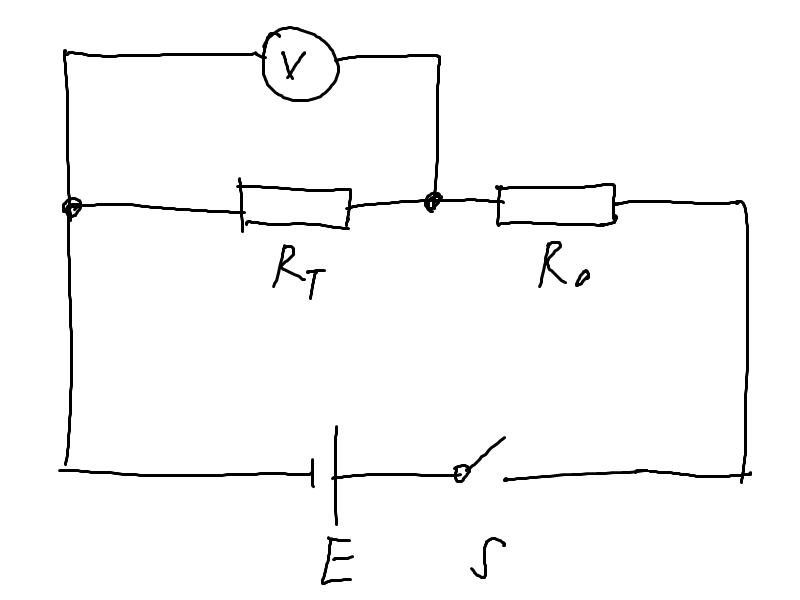
\includegraphics[width=0.33\linewidth]{fig/temp-detector.png}
\caption{一个肥硕的电路}
\label{fig-temp-detector}
\end{figure}

这个电路可以作为温度传感器,$V$的示数为$U_T(T)=\frac{E R_T}{R_T+R_0}$,温度越高,$U_T$越大。

温度改变$\Delta T$时,$\Delta U_T=\frac{E R_0}{(R_T+R_0)^2} \frac{\partial R_T}{\partial T} \Delta T$。我们把$\frac{\Delta U_T}{\Delta T}=\frac{E R_0}{(R_T+R_0)^2} \frac{\partial R_T}{\partial T}$称为传感器的灵敏度,$\Delta T$相同时,灵敏度越大,$\Delta U_T$就越大。

$\frac{\partial R_T}{\partial T}$越大,灵敏度就越大,这符合直觉。还可以发现常温下的电阻$R_T$越大,灵敏度越小。如果可以选择不同的$R_0$,那么$R_0=R_T$时灵敏度最大,因为
\begin{equation*}
\frac{R_0}{(R_T+R_0)^2}=\frac{1}{R_0+\frac{R_T}{R_0}+2 R_T}
\end{equation*}
\section{有效数字}
上面说了通过被测量的最大误差计算结果的最大误差的方法。有效数字是一种更加方便但不精确的方法,相当于把绝对误差当成最后一位数字。比如$x=1.23 \times 10^3$其实表示$1.225 \times 10^3 \le x <1.235 \times 10^3$,绝对误差为$0.01 \times 10^3=10$。有效数字从最左边的不为$0$的数字到最右边的数字为止,这些数字的个数称为有效位数。

几个量加减的时候有效数字取绝对误差大的,几个量乘除的时候有效数字取相对误差大的(也就是有效位数少的)。比如$1.23 \times 10^3+8.9 \times 10^1=1.32 \times 10^3$,而$1.23 \times 10^3 \times 8.9 \times 10^1=1.1 \times 10^5$。

一般认为幂函数、指数函数、对数函数和三角函数的有效位数就是自变量的有效位数。如果需要更精确,还是老老实实算导数吧。

如果用同一个仪器测量多组数据,它们的有效位数不同(比如测电流从$1.2 \unit{A}$测到$12.3 \unit{A}$),有时候会统一按照有效位数最多的值计算(传说是为了让结果更好看),更精确的实验会单独计算每组数据的误差。

画图时坐标轴的有效位数有人认为要与测得的数据相同,有人认为应该根据方格纸的最小刻度和估读确定,更精确的实验会在每个数据点附近标出它的误差范围。
\section{误差的来源}
$x$是测量得到的值,那么怎么确定最大误差$\Delta x$呢?偶然误差可以分为两部分:一是统计误差,也就是多次测量时每次测得的值不同造成的;二是仪器误差,也就是每次测量时仪器的最小刻度等等造成的。(专业一点叫作\emph{A类不确定度}和\emph{B类不确定度})

仪器误差比较容易理解,一般取的是仪器的最小刻度,要估读就取估读出的最小刻度。但是也有一些约定俗成的取法,比如钢尺是$0.1 \unit{mm}$,游标卡尺是$0.02 \unit{mm}$,螺旋测微器是$0.004 \unit{mm}$,秒表是$0.5 \unit{s}$(人的反应时间)。专业的仪器生产厂商会在仪器上标出仪器误差。

讲统计误差需要一些统计学的知识。比如你用刻度尺测一只虫子的长度,测量$3$次分别是$1.05 \unit{cm}$,$1.04 \unit{cm}$,$1.06 \unit{cm}$,你觉得不够,再测量$3$次分别是$1.02 \unit{cm}$,$1.08 \unit{cm}$,$1.05 \unit{cm}$。前$3$次和总共$6$次的平均值都是$1.05 \unit{cm}$,而且前$3$次的结果相互之间比较接近,统计误差应该比较小。

这里我不打算讲统计误差的计算公式,可以粗略地认为是这些数据的标准差。(也就是方差开根号,但是严格的定义有所不同)

但是!我们认为测$6$次比测$3$次更好。虽然统计误差变大了,但是真实值更有可能落在误差范围内。如果只测$3$次,你得到的测量值可能如图\ref{fig-error-range},$3$次的测量值都比真实值大。而且相互接近,完全有可能出现这样的偶然情况。(在没有系统误差的前提下)如果增加测量次数,可能会测出偏小的值,这样真实值就更有可能落在误差范围内。
\begin{figure}[htb]
\centering
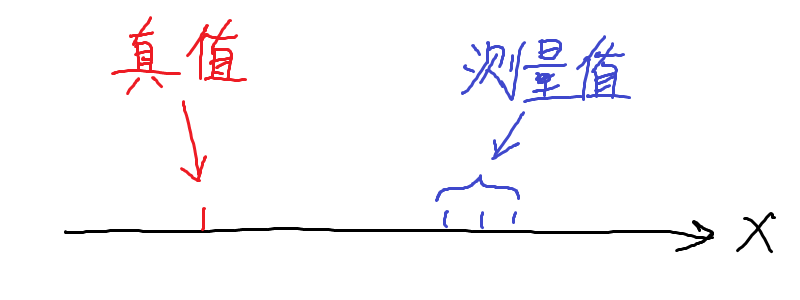
\includegraphics[width=0.33\linewidth]{fig/error-range.png}
\caption{一个RP不足的同学测出的结果}
\label{fig-error-range}
\end{figure}

多次测量取平均值并不能减小仪器误差。比如$\overline{x}=\frac{1}{n}(x_1+x_2+\dots+x_n)$,而每次测量的仪器误差$\Delta x_1,\Delta x_2,\dots,\Delta x_n$都是$\Delta x$,那么$\Delta \overline{x}=\frac{1}{n} n \Delta x=\Delta x$。多次测量取平均值也不一定会减小统计误差,它的真正意义是让平均值和统计误差变得更合理,接下来仔细讲一下这件事情。

(许多高考实验题的误差范围都是出题人一拍脑袋想出来的,说明他们的物理素养不高)
\section{正态分布;置信度}
如果对一个物理量进行多次测量,测量值会满足一定的分布。最常见的是正态分布,又叫高斯分布:(什么你要萝莉分布?我这里没有)
\begin{equation*}
P(x)=\frac{1}{\sqrt{2 \pi} \sigma} \rme^{-\frac{(x-x_0)^2}{2 \sigma^2}}
\end{equation*}

这个式子看起来很厉害,但是不要怕,不要怕,不要怕。它的图像大致如图\ref{fig-gaussian}:
\begin{figure}[htb]
\centering
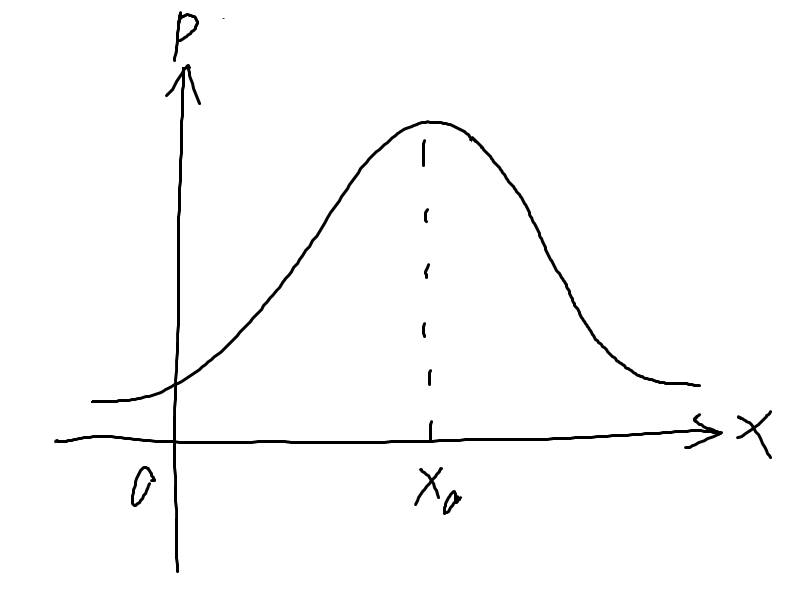
\includegraphics[width=0.33\linewidth]{fig/gaussian.png}
\caption{画得好像不是很对称}
\label{fig-gaussian}
\end{figure}

如果一个物理量的真实值为$x_0$,对它进行测量,测量值为$x$的概率就是$P(x)$。进行的测量次数越多,平均值就越接近$x_0$,标准差越接近$\sigma$,详细的证明以后再讲。(需要很复杂的积分,估计是有生之年)

$x_0$和$\sigma$这两个参量可以确定一个正态分布,$x_0$确定峰的左右位置,$\sigma$确定峰的宽度。因为概率的归一化,只要峰的宽度确定了,峰的高度就确定为$\frac{1}{\sqrt{2 \pi} \sigma}$。

$\sigma$是由被测量、仪器、测量方法等等决定的。比如一只虫子在$1 \unit{cm}$范围内抖动,你测量它的位置,$\Delta x$就大约有$1 \unit{cm}$,如果测出来$\Delta x$只有$0.01 \unit{cm}$反而不符合事实,但是我们仍然可以测出虫子位置的平均值。再比如一根圆柱体的表面凹凸不平,你在不同方向测量它的直径就会得到不同的值。所以说统计误差不是越小越好,多次测量取平均值可以让平均值和统计误差变得更合理。

事实上不同的仪器有不同的误差分布,正态分布只是一个近似。比如测量长度怎么也不可能小于$0$,但是正态分布在小于$0$的地方还是有的,只是概率很小而已。对一些标准量进行测量可以证明,正态分布在大多数情况下是很好的近似。比如扔$n$次硬币有$k$次正面朝上的概率为$P(k)$(没错就是二项式分布),当$n$很大时,$P(k)$接近正态分布,$k=\frac{n}{2}$的地方最大,向两边减少。

如果已知$x_0$和$\sigma$,可以求出$x$为某个值$x_1$的概率。但是做实验做的其实是相反的事情:已知测量值$x_1,x_2,\dots,x_n$,假设$x$满足正态分布,求$x_0$和$\sigma$分别为某个值$x_{0 1}$和$\sigma_1$的概率。通过解含有随机变量的方程可以把$x_0$和$\sigma$的分布函数算出来,但是这个计算很复杂。

知道了$x_0$和$\sigma$的分布,就可以计算置信度CI,它可以描述测量结果的准确程度。比如置信度为95\%表示区间$(\overline{x}-\Delta x,\overline{x}+\Delta x)$有95\%的可能性覆盖到了真实值$x_0$。

置信度与测量次数$n$和最大误差$\Delta x$有关,$n$越大,或者$\Delta x$越大,那么置信度越大。具体的计算也很复杂,实际工作中一般可以查表。

实验永远不能100\%保证真实值是多少,只能给出这样的一个概率,除非$\Delta x$无穷大,覆盖整条数轴。现代粒子物理的置信度一般是90\%或者95\%,火箭之类的精密工程甚至可以达到99.9999\%。
\section{仪器的分辨率}
仪器的分辨率大致就是最小刻度,也有些地方的定义是最小刻度的倒数。最小刻度不可能无限减小,总有一些物理规律限制它。(所以分辨率应该是越小越好还是越大越好呢)

光学实验中限制分辨率的一个重要原因是衍射。比如显微镜需要用光照亮物体(或者电子束衍射之类的),如果用可见光,波长约为$500 \unit{nm}$,比波长更小的物体衍射现象就会很明显,看不清楚。如果减小波长,光的衍射现象会减弱,但是光的动量就变大了,撞到物体上对它的影响会增强,测量结果会受到量子力学中不确定性原理$\Delta x \Delta p \le \frac{\hbar}{2}$的限制。

有些实验仪器需要用透镜把光汇聚到一个点上,但是因为衍射,这个点不可能无限小。道理跟小孔成像是一样的,虽然透镜比小孔大得多,但是衍射现象仍然存在。如果光的波长是$\lambda$,透镜的大小是$D$,焦距是$f$,那么衍射范围的大小$d=\frac{\lambda f}{D}$。

这里透镜的大小(专业一点叫\emph{线度})可以是圆形的直径、半径,或者正方形的边长等等,只要量纲是长度就行,先不管前面的系数。可以看出,$\lambda$越大,$D$越小,衍射就越明显。

在精密的力学实验中,限制分辨率的一个重要原因是热运动。比如用一把尺子测一根杆子的长度,要把整个实验装置放到低温环境中,来减小尺子和杆子的热运动。但是!你还记得前面讲的热波长吗?温度降低,尺子和杆子的热波长就会增大,测量结果仍然受到不确定性原理的限制。

前面说的都是空间分辨率,计时的仪器也有时间分辨率。比如高考范围内的打点计时器每隔$0.02 \unit{s}$打一个点,如果每两个点的距离相等,我们就认为物体在匀速运动。其实如果物体的速度在快速变化,而变化的时间小于$0.02 \unit{s}$,用打点计时器是看不出来的。(如果你熟悉傅立叶变换,可以认为打点计时器过滤了速度的高频分量)

多次测量取平均值可以理解为牺牲时间分辨率来换取空间分辨率。

\chapter{解析几何}
\section{平面上直线的方程;无穷远处的东西}
(接下来好像是高考能用得到的黑科技,但是需要先看前面的线性代数,以及理论力学关于自由度的内容)

在二维平面上,一个点有两个自由度,也就是说确定它的坐标需要两个参数。无论用直角坐标、极坐标还是其他奇怪的坐标,要确定一个点在平面上的位置都需要两个参数,而且这两个参数可以(一一对应地)表示平面上的所有点。(极坐标规定$r \ge 0$,$\theta \in [0,2 \pi)$,且在$r=0$时$\theta=0$,否则就不是一一对应。其他奇怪的坐标需要更奇怪的定义域)

平面上的一条直线在直角坐标系中可以表示为$A x+B y+C=0$,$A,B$不全为$0$。这是一个约束条件,剩下一个自由度,而确定一个点在直线上的位置确实需要一个参数。比如确定了$x$,用这个方程可以解出$y$,那么点在平面上的位置就确定了。

为什么说这个方程表示一条直线呢?这就不是数学的问题了,我们可以随便定义“直线”这个概念。方程$A x+B y+C=0$放到直角坐标系里看起来是直的,符合我们的直觉。以后我们还会遇到把$(x-x_0)^2+(y-y_0)^2=r^2$这样的方程称为“直线”的情况。

可以把$A x+B y+C=0$改写为$\xi x+\eta y=1$,其中$\xi=-\frac{A}{C}$,$\eta=-\frac{B}{C}$,而且$\xi$和$\eta$不全为$0$。每组$(\xi,\eta)$对应一条不过原点的直线,也就是说平面上所有不过原点的直线可以用两个参数表示。上面的$A,B,C$三个参数中,只有两个是独立的。

($\xi$读作xi,克赛,$\eta$读作eta,伊塔,它们分别与英文字母x、y对应)

但是“不全为$0$”和“不过原点”放在这里很不爽!先考虑这样的情况:$\xi=\eta=a>0$,它表示一条斜着的直线。$a$越小,这条直线离原点越远。如果$a=0$,可以认为它表示一条无穷远处的直线。无穷远处的直线只有一条,不管它是从哪个方向移到无穷远的,都是同一条。

如果$\xi=\infty$,$\eta=\infty$,那么它表示一条过原点的直线。但是过原点的直线有无穷多条,好在无穷大也是有大小之分的,这条直线的斜率$k=-\frac{\xi}{\eta}$,跟普通直线的斜率定义一样。(虽然我还没讲过无穷大的严格定义是什么,两个无穷大的比值应该在讲极限的时候讲。$k$可能是$0$或者$\infty$)

平面上的一个点可以表示为(x,y),跟上面对应,$x=y=0$时,它就是原点,只有一个;$x=\infty$,$y=\infty$时,它表示一个无穷远处的点,或者说无穷远直线上的点,这样的点有无穷多个。

这样就有了奇怪的对称性:过每个点的直线都有无穷多条,每条直线上的点都有无穷多个,过两个点的直线有且只有一条,两条直线的交点有且只有一个。(包括原点、无穷远点、过原点的直线、无穷远直线)

这些无穷远处的东西是射影几何研究的内容,我们以后再讲,一般的解析几何不会考虑。高考很喜欢在这种地方挖坑。

顺便说一句,一个复数相当于两个实数,所以用一个复参数可以表示复平面上的所有点。
\section{空间中平面和直线的方程}
在三维空间中,一个点有三个自由度,可以类似地发现方程$A x+B y+C z+D=0$表示一个平面,它是一个约束条件,剩下两个自由度。三维空间中所有不过原点的平面可以用三个参数表示。

它的法向量$\mathbf{n}$平行于$(A,B,C)$。如果有一个矢量$\mathbf{a}$满足$\mathbf{n} \cdot \mathbf{a}=A a_x+B a_y+C a_z=0$,那么$\mathbf{a}$与平面平行。

如果一个不过原点的平面在$x,y,z$轴上的截距分别是$x_0,y_0,z_0$,它的方程就是$\frac{x}{x_0}+\frac{y}{y_0}+\frac{z}{z_0}=1$,但是过原点的平面就不能这么算了。(化竞似乎学过一种叫晶格指数的东西)

平面上点到直线的距离是$\frac{|A x_0+B y_0+C|}{\sqrt{A^2+B^2}}$,平行直线的距离是$\frac{|C_1-C_2|}{\sqrt{A^2+B^2}}$。类似地,空间中点到平面的距离是$\frac{|A x_0+B y_0+C z_0+D|}{\sqrt{A^2+B^2+C^2}}$,平行平面的距离是$\frac{|D_1-D_2|}{\sqrt{A^2+B^2+C^2}}$。这些公式很容易推广到高维空间。

三维空间中的直线需要两个约束条件,比如
\begin{equation*}
\begin{cases}
A_1 x+B_1 y+C_1 z+D_1=0 \\
A_2 x+B_2 y+C_2 z+D_2=0
\end{cases}
\end{equation*}

也就是两个平面相交得到一条直线。但是如果这两个平面平行,就不能表示一条直线了。(不考虑无穷远处的东西)

也可以用矢量表示:$\mathbf{a}+\lambda \mathbf{b}$,用分量表示就是
\begin{equation*}
\begin{cases}
x=a_x+\lambda b_x \\
y=a_y+\lambda b_y \\
z=a_z+\lambda b_z
\end{cases}
\end{equation*}

这样用了六个参数$a_x,a_y,a_z,b_x,b_y,b_z$来确定一条直线,而$\lambda$用来确定直线上的点。但是把$\mathbf{b}$乘上一个倍数,或者把$\mathbf{a}$换成$\mathbf{a}+\mathbf{b}$,直线不会改变,这说明有两个参数不是独立的。

在三维空间中表示一条直线只需要四个独立的参数,可以这样想:两点确定一条直线,这两个点共有六个自由度。但是把第一个点沿着直线移动,直线不会改变,第二个点也是一样,这样就少了两个自由度,剩下四个自由度。

空间中点到直线的距离好像没有容易背的公式,可以用投影来算。
\section{三点共线和相关的东西}
在平面上,三个点的坐标为$P_1(x_1,y_1),P_2(x_2,y_2),P_3(x_3,y_3)$,如果它们共线,可以表示为$\frac{y_1-y_2}{x_1-x_2}=\frac{y_1-y_3}{x_1-x_3}$。但是这样对下标$1,2,3$不对称,还会遇到分母为$0$的问题。一种更炫酷的表示方法是
\begin{equation*}
\begin{vmatrix}
x_1 & y_1 & 1 \\
x_2 & y_2 & 1 \\
x_3 & y_3 & 1
\end{vmatrix}=0
\end{equation*}

如果你熟悉行列式的运算技巧,可以理解为第三行等于$\lambda$倍的第一行加$1-\lambda$倍的第二行,也就是说$P_3$在直线$P_1 P_2$上。

现在我们从第一种表示推导第二种表示。设$\frac{y_1-y_2}{x_1-x_2}=\frac{y_1-y_3}{x_1-x_3}=k$,那么$k x_1-y_1=k x_2-y_2$。设$k x_1-y_1=m$,那么$x_1 \cdot \frac{k}{m}+y_1 \cdot -\frac{1}{m}+1 \cdot -1=0$。同理,$x_2 \cdot \frac{k}{m}+y_2 \cdot -\frac{1}{m}+1 \cdot -1=0$,$x_3 \cdot \frac{k}{m}+y_3 \cdot -\frac{1}{m}+1 \cdot -1=0$。

也就是说,存在一组实数$(a_1,a_2,a_3)=(\frac{k}{m},-\frac{1}{m},-1)$,它们满足线性齐次方程组
\begin{equation*}
\begin{cases}
x_1 a_1+y_1 a_2+a_3=0 \\
x_2 a_1+y_2 a_2+a_3=0 \\
x_3 a_1+y_3 a_2+a_3=0
\end{cases}
\end{equation*}

注意在这个方程组中,$x$和$y$是已知的系数,$a$是未知量。在线性代数那章讲过,要让这个方程组有解,系数行列式必须为$0$,于是就有了三点共线的第二种表示。

举个栗子:已知直线$l$经过$A(1,2),B(3,4)$,它与直线$y=5x+6$交于$C$,求$C$的坐标。(我编出来的系数就是这么普通)

我们不用算出$l$的方程,直接用行列式来做。设$C(x,5x+6)$,$\begin{vmatrix}
1 & 2 & 1 \\
3 & 4 & 1 \\
x & 5x+6 & 1
\end{vmatrix}=0$,把行列式算出来得到$8x+10=0$,$x=-\frac{5}{4}$,$C(-\frac{5}{4},-\frac{1}{4})$。

平面上的三个点共有六个自由度,三点共线是一个约束条件,剩下五个自由度。我已经在很多地方强调过,自由度的数量可以用来判断一道题能不能做出来,一般情况下$n$个方程能且只能解出$n$个未知数。高中物理题有时候会出现多出来的条件,有时候会自相矛盾,更麻烦的是有时候条件不够,而且真正的高考和竞赛里确实出现过这样的情况,我也不知道该怎么办。

如果把刚才的方程组看成关于$k$和$m$的方程组,那么有两个未知数,但是有三个方程,一般是无解的,除非出现特殊情况,这里的特殊情况就是三点共线。

如果有三条直线$l_1:\xi_1 x+\eta_1 y=1,l_2:\xi_2 x+\eta_2 y=1,l_3:\xi_3 x+\eta_3 y=1$,这三条线共点可以类似地表示为
\begin{equation*}
\begin{vmatrix}
\xi_1 & \eta_1 & 1 \\
\xi_2 & \eta_2 & 1 \\
\xi_3 & \eta_3 & 1
\end{vmatrix}=0
\end{equation*}

在三维空间中,四点共面可以类似地写成
\begin{equation*}
\begin{vmatrix}
x_1 & y_1 & z_1 & 1 \\
x_2 & y_2 & z_2 & 1 \\
x_3 & y_3 & z_3 & 1 \\
x_4 & y_4 & z_4 & 1
\end{vmatrix}=0
\end{equation*}

但是如果不熟悉四阶行列式的计算,可能还是先用三个点求出平面的方程,再把第四个点代进去比较方便。你猜四个平面共点怎么表示?

三维空间中的三点共线和三面共线都相当于两个约束条件,好像没有比较对称的表示方法,如果有人知道欢迎来告诉我。
\section{叉积}
二维矢量的叉积是一个标量,$\mathbf{a} \times \mathbf{b}=a_x b_y-a_y b_x$。它满足反交换律$\mathbf{a} \times \mathbf{b}=-\mathbf{b} \times \mathbf{a}$和分配律$\mathbf{a} \times (\mathbf{b}+\mathbf{c})=\mathbf{a} \times \mathbf{b}+\mathbf{a} \times \mathbf{c}$。

三维矢量的叉积是一个矢量,$\mathbf{a} \times \mathbf{b}=(a_y b_z-a_z b_y,a_z b_x-a_x b_z,a_x b_y-a_y b_x)$。它满足反交换律和分配律,一般不满足结合律。用多了之后这个公式就背下来了。

设$\mathbf{c}=\mathbf{a} \times \mathbf{b}$,你可以验证一下$\mathbf{c} \perp \mathbf{a}$且$\mathbf{c} \perp \mathbf{b}$。在右手系中,$\mathbf{c}$的方向可以用右手螺旋来判断:把右手四指指向$\mathbf{a}$的方向,然后转向$\mathbf{b}$的方向,大拇指的方向就是$\mathbf{c}$的方向。

很多物理公式要用叉积才能严格表示出矢量的方向,比如洛伦兹力$\mathbf{F}=q \mathbf{v} \times \mathbf{B}$,安培力$\mathbf{F}=I \mathbf{L} \times \mathbf{B}$(电流$I$是标量,而$\mathbf{L}$的方向是电流方向),力矩$\mathbf{M}=\mathbf{r} \times \mathbf{F}$等等。但是如果你习惯用右手定则左手定则之类的判断它们的方向,那就不用管右手螺旋了,以免搞混。

如果平行四边形的两条邻边分别是矢量$\mathbf{a},\mathbf{b}$,那么它的面积是$|\mathbf{a} \times \mathbf{b}|$(二维情况下是取绝对值,三维情况下是取模长),三角形的面积要除以$2$。

如果平行六面体从一个顶点出发的三条边分别是矢量$\mathbf{a},\mathbf{b},\mathbf{c}$,那么它的体积是$|\mathbf{a} \times \mathbf{b} \cdot \mathbf{c}|=\left| \begin{vmatrix}
a_x & a_y & a_z \\
b_x & b_y & b_z \\
c_x & c_y & c_z
\end{vmatrix} \right|$,三棱柱的体积要除以$2$,三棱锥的体积要除以$6$。

$\mathbf{a} \times \mathbf{b} \cdot \mathbf{c}$称为矢量三重积,它是一个标量,可正可负。你可以验证一下矢量三重积和行列式的结果是一样的,并且$\mathbf{a} \times \mathbf{b} \cdot \mathbf{c}=\mathbf{b} \times \mathbf{c} \cdot \mathbf{a}=-\mathbf{b} \times \mathbf{a} \cdot \mathbf{c}$。

高考立体几何经常让你算二面角,我个人用的都是建系暴算。知道一个面的两条边对应的矢量,就能用叉积算出它的法向量,而不用解方程组。如果觉得直接算出来的法向量太难看,可以乘一个(正的)倍数变得好看一点。而且这样算出来的法向量的方向可以用右手螺旋确定,就不用凭感觉判断是锐角还是钝角了。算出法向量之后记得在图中对照一下,特别是平行于坐标轴或者垂直于坐标轴的情况。如果你不熟悉这种做法,可以随便找几道立体几何题试一下。

一条直线把平面分成两部分,设直线上有一点$O$,平面上有一点$P$,可以用叉积表示$P$在直线的哪一侧:取平行于直线的向量$\mathbf{n}$,然后计算$\Delta=\mathbf{OP} \times \mathbf{n}$,如果$\Delta>0$,那么$P$在直线的一侧;如果$\Delta<0$,那么$P$在另一侧;如果$\Delta=0$,那么$P$在直线上。

而左侧和右侧是人为定义的,如果定义$\Delta>0$的部分是左侧,那么$\Delta<0$就是右侧。

一个平面把三维空间分成两部分,可以在平面上取两个方向不同的向量$\mathbf{n}_1,\mathbf{n}_2$,计算三重积$\Delta=\mathbf{OP} \times \mathbf{n}_1 \cdot \mathbf{n}_2$,然后进行类似的分类。在3D的游戏中,我们经常看到一个面的两侧显示不同的颜色,电脑就是这样判断一个面的两侧的。
\section{坐标变换的代数性质}
平移、旋转不会改变线段的长度,也不会改变两条直线的夹角。如果把坐标轴缩放一下,线段的长度和两条直线的夹角会改变,但是原来平行的线段仍然平行。

平移、旋转和缩放统称为线性变换,或者叫仿射变换。在线性代数那章讲过,坐标变换对矢量的效果可以用矩阵表示,但是平移对矢量是没有用的,所以只有旋转和缩放。现在我们考虑点而不是矢量,平移会改变点相对于坐标原点的位置。平面上的线性变换可以写成
\begin{equation*}
\begin{cases}
x'=a_{1 1} x+a_{1 2} y+c_1 \\
y'=a_{2 1} x+a_{2 2} y+c_2
\end{cases}
\end{equation*}

$c_1$和$c_2$表示平移的效果。

线性变换不会改变曲线的方程的次数,直线变换之后还是直线,二次曲线变换之后还是二次曲线。事实上,椭圆(包括圆)变换之后还是椭圆,抛物线变换之后还是抛物线,双曲线变换之后还是双曲线。因此线性变换把所有二次曲线分成了椭圆、抛物线、双曲线三类。(除了一些特殊情况,或者说\emph{退化}的情况,包括空集、一个点、一条直线、两条平行直线、两条相交直线)

如果二次曲线的方程是$A x^2+B x y+C y^2+D x+E y+F=0$,设$\Delta=\begin{vmatrix}
2 A & D & B \\
D & 2 C & E \\
B & E & 2 F
\end{vmatrix}$,$\delta=\begin{vmatrix}
2 A & B \\
B & 2 C
\end{vmatrix}$,可以这样判断:当$\Delta \neq 0$时,如果$\delta>0$,则是椭圆或者空集(具体是哪种可以配方试试看);如果$\delta=0$,则是抛物线;如果$\delta<0$,则是双曲线;当$\Delta=0$时,则是退化的情况。椭圆、抛物线、双曲线分别对应$\delta>0$、$\delta=0$、$\delta<0$三种情况,所以二次曲线只有这三类。

线性变换不会改变两条曲线的交点数量,特别是相切的曲线变换之后还是相切。与椭圆有关的问题可以缩放坐标轴,把它变成一个圆,特别是与平行和相切有关的问题。

有人认为,几何学研究的是变换下的不变性,不同的几何学研究不同的变换。比如欧氏几何研究长度、角度这些平移、旋转(或者叫正交变换)下的不变性,射影几何研究平行、交比这些射影变换下的不变性,拓扑几何研究一个面上有几个洞这些拓扑变换下的不变性。而每种变换都是可以用代数方法描述的,这样就在代数与几何之间建立起了联系。反过来也可以用几何方法来研究代数问题,比如一些不满足交换律的代数可以用空间中的旋转(或者爸爸和妈妈)表示,对$c$取模的代数可以用周长为$c$的圆圈表示。这就是传说中的\emph{爱尔兰根纲领},是现代数学研究十分重要的方向。
\section{五个点确定一条二次曲线}
刚才讲了平面上二次曲线一般的方程:$A x^2+B x y+C y^2+D x+E y+F=0$。如果$A,B,\dots,F$同时乘一个倍数,表示的还是原来的二次曲线,所以这六个参数中只有五个是独立的。因此我们可以猜:五个点确定一条过这五个点的二次曲线,道理跟两个点确定一条直线差不多。

我们在平面上取五个点$P_1,P_2,\dots,P_5$,要求任意三个点不共线。过$P_1,P_2$作直线$l_1$,设它的方程为$l_{1 1} x+l_{1 2} y+l_{1 3}=0$。我们把代数式$l_{1 1} x+l_{1 2} y+l_{1 3}$也称为$l_1$,也就是说直线$l_1$的方程为$l_1=0$。(接下来不区分直线$l_1$,代数式$l_1$和方程$l_1=0$,可以根据上下文判断)然后过$P_3,P_4$作$l_2$,过$P_1,P_3$作$l_3$,过$P_2,P_4$作$l_4$。

现在看这个式子:$S=l_1 l_2+\lambda l_3 l_4$,$\lambda$是一个待定系数。这是关于$x,y$的二次式(除了退化的情况),而且把$P_1,P_2,P_3,P_4$代进去都得到$0$,也就是说这是一条过$P_1,P_2,P_3,P_4$的二次曲线。既然任意三个点不共线,$P_5$代进去一般不能得到$S=0$,这时令$S=0$可以解出$\lambda$,也就确定了这条二次曲线。所以说,如果五个点中任意三个点不共线,那么有且只有一条二次曲线过这五个点。

用类似的方法可以证明,如果九个点中任意三个点不共直线(或者说一次曲线),并且任意六个点不共二次曲线,那么有且只有一条三次曲线过这九个点。你可以想想更高次和零次的情况。

在高斯的时代,九个点能否确定一条三次曲线引起过很大的争论,况且实际问题中的九个点一般会有六个点共二次曲线。这个问题最简单的想法是把九个点代进三次曲线的一般方程,然后用九个方程解出九个待定系数。然而这九个方程不一定是独立的,这一点用肉眼当然很难看出来,因此这个问题推动了线性代数的发展,这又是一个代数和几何相结合的例子。

(以后应该专门有一章射影几何,奇怪的空间曲面也要以后再讲)

\chapter{数列}
\section{差分与求和}
如果有一个数列$\{a_n\}$,可以定义它的差分$\Delta a_n=a_n-a_{n-1}$,求和$\Sigma a_n=a_1+a_2+\dots+a_n$。(它们是一对逆运算,$\Delta \Sigma a_n=a_n$。有些地方会定义$\Delta a_n=a_{n+1}-a_{n}$,这样不太方便。)

比如$\Delta n^2=2 n-1$,$\Sigma n^2=\frac{1}{6}n(n+1)(2 n+1)$。像$n^4+2 n^3+3 n$这样的多项式可以一项一项差分或者求和,也就是说差分与求和都是线性算符。

差分算符$\Delta$与求和算符$\Sigma$跟求导算符$\ddx$与积分算符$\int \opd x$很像。这个积分算符表示的是不定积分,所以这个求和算符其实是“不定”求和。比如“定”求和$\sum_{n=38}^{62} n^2$用这个求和算符就要表示成$\Sigma n^2|_{n=62}-\Sigma n^2|_{n=37}$。数列差分与求和的时候,下标加减$1$的情况比微积分还要麻烦。

上面的求和是从$1$开始的,其实不一定要从$1$开始,相当于“不定”求和出来的常数换一下,对计算“定”求和没有影响。

如果要与微积分更像一点,可以把差分与求和写成$\frac{\Delta}{\Delta n}$与$\Sigma \Delta n$。但是一般情况下$\Delta n=1$,所以可以省略,否则要进行换元。比如$1+3+5+\dots$可以表示成$\Sigma n \Delta n$,其中$\Delta n=2$。令$n=2 m-1$,这样$m=\frac{n+1}{2}$,$\Delta m=\frac{1}{2} \Delta n=1$,而且$m=1$时$n=1$,这样“不定”求和的起点是一致的。换元之后就得到$\Sigma n \Delta n=\Sigma (2 m-1) \Delta m=2 \cdot \frac{1}{2} m(m+1) -m=m^2=\frac{(n+1)^2}{4}$。
\section{用递推求$\Sigma n^p$}
我们都知道$\Sigma n=\frac{1}{2}n(n+1)$,现在来推导$\Sigma n^2$。我们不直接考虑$\Sigma n^2$,而是先考虑$\Sigma n^3$:
\begin{align*}
\Sigma n^3+(n+1)^3&=\sum_{k=1}^{n+1} k^3 \\
&=\sum_{k=0}^n (k+1)^3 \\
&=\sum_{k=0}^n (k^3+3 k^2+3 k+1) \\
&=\Sigma n^3+3 \Sigma n^2+\frac{3}{2}n(n+1)+(n+1)
\internote{(两边的$\Sigma n^3$可以消掉,$\sum_{k=0}^n 1=n+1$)}
3 \Sigma n^2&=(n+1)^3-\frac{3}{2}n(n+1)-n-1 \\
\Sigma n^2&=\frac{n^3}{3}+\frac{n^2}{6}+\frac{n}{2} \\
&=\frac{1}{6}n(n+1)(2 n+1)
\end{align*}

用类似的方法,对任何正整数$p$,如果知道$\Sigma n,\Sigma n^2,\dots,\Sigma n^{p-1}$,就能求出$\Sigma n^p$。这是一种递推的方法,而且第二步打开$(k+1)^{p+1}$需要计算组合数,当$p$增大的时候需要很大的计算量。

【练习】证明$\Sigma n^3=\frac{1}{4}n^2 (n+1)^2$。

并没有简单(复杂度与$p$无关)的公式可以计算$\Sigma n^p$。如果$p$是实数甚至复数,问题就更复杂了。传说中的\emph{黎曼zeta函数}就是$\zeta(z)=\sum_{k=0}^{\infty} k^z$,在现代数学中十分重要。一个简单的结论是:$z$是实数且$z<-1$时,$\zeta(z)$收敛;$z \ge -1$时,$\zeta(z)$发散。
\section{降幂;离散微积分}
再来讲另一种计算$\Sigma n^p$的方法。先定义一个“降幂”运算:$\dspw{n}{p}=n \cdot (n-1) \cdot (n-2) \cdot \dots \cdot (n-p+1)$,其中$n$是实数,$p$是正整数。比如$\dspw{n}{4}=n(n-1)(n-2)(n-3)$。(也可以定义“升幂”,但是不常用)

然后我们发现了喜闻乐见的事情:$\Delta \dspw{n}{p}=p \dspw{(n-1)}{p-1}$,$\Sigma \dspw{n}{p}=\frac{1}{p+1} \dspw{(n+1)}{p+1}$。这两个公式和微积分里的差不多,但是要注意$n$的加减。

举个栗子,$\Delta \dspw{n}{3}=n(n-1)(n-2)-(n-1)(n-2)(n-3)=3(n-1)(n-2)=3 \dspw{(n-1)}{2}$。直接计算降幂的求和可以用一加一减的技巧,比如
\begin{align*}
\Sigma \dspw{n}{2}&=2 \cdot 1+3 \cdot 2 +\dots+ n(n-1) \\
&=\frac{1}{3}(3 \cdot 2 \cdot 1-2 \cdot 1 \cdot 0+4 \cdot 3 \cdot 2-3 \cdot 2 \cdot 1+\dots+(n+1)n(n-1)-n(n-1)(n-2)) \\
&=\frac{1}{3}(n+1)n(n-1) \\
&=\frac{1}{3} \dspw{(n+1)}{3}
\end{align*}

因为求和的下限是$2$,这个结果在$n \ge 2$时成立,$n=1$时要另外讨论。

组合数中经常出现$n \cdot (n-1) \cdot (n-2) \dots$这样的式子,如果你熟悉组合数的公式,可以推导出这两个公式。

降幂的差分与求和容易计算,但是把普通的幂转换成降幂是不容易的,可以用类似于整式除法的方法,比如$n^2=\dspw{n}{2}+\dspw{n}{1}$,$n^3=\dspw{n}{3}+3 \dspw{n}{2}+\dspw{n}{1}$,$n^4=\dspw{n}{4}+6 \dspw{n}{3}+7 \dspw{n}{2}+\dspw{n}{1}$。

有兴趣的同学可以把$\Sigma n^3,\Sigma n^4$推导一遍,还可以检验一下这种方法的复杂度和递推是一样的。

到现在为止$p$是正整数,如果$p$是$0$或者负整数怎么办呢?因为$\frac{\dspw{n}{p}}{\dspw{n}{p-1}}=n-p+1$,令$p=1$,得到$\frac{\dspw{n}{1}}{\dspw{n}{0}}=n$,所以$\dspw{n}{0}=1$。类似地可以定义$\dspw{n}{-1}=\frac{1}{n+1},\dspw{n}{-2}=\frac{1}{(n+1)(n+2)},\dots$

上面的差分与求和公式仍然成立,现在直接计算降幂的求和可以通过裂项,比如
\begin{align*}
\Sigma \dspw{n}{-3}&=\frac{1}{1 \cdot 2 \cdot 3}+\frac{1}{2 \cdot 3 \cdot 4}+\dots+\frac{1}{(n+1)(n+2)(n+3)} \\
&=\frac{1}{2}(\frac{1}{1 \cdot 2}-\frac{1}{2 \cdot 3}+\frac{1}{2 \cdot 3}-\frac{1}{3 \cdot 4}+\cdots+\frac{1}{(n+1)(n+2)}-\frac{1}{(n+2)(n+3)}) \\
&=\frac{1}{2}(\frac{1}{2}-\frac{1}{(n+2)(n+3)})
\end{align*}

这里求和的下限是$0$。因为是“不定”求和,可以去掉括号中的$\frac{1}{2}$,得到$\Sigma \dspw{n}{-3}=\frac{1}{-2} \cdot \frac{1}{(n+2)(n+3)}=\frac{1}{-2}\dspw{(n+1)}{-2}$。在计算“定”求和时仍然要注意边界,比如$\frac{1}{1 \cdot 2 \cdot 3}+\frac{1}{2 \cdot 3 \cdot 4}+\dots+\frac{1}{(n-2)(n-1)n}=\Sigma \dspw{k}{-3}|_{k=n-3}-\Sigma \dspw{k}{-3}|_{k=-1}=\frac{1}{-2}(\dspw{0}{-2}-\dspw{(n-2)}{-2})=\frac{1}{-2}(\frac{1}{1 \cdot 2}-\frac{1}{(n-1)n})$。

但是!$p=0$时,$\Delta \dspw{n}{p}=\Delta 1=0$。$p=-1$时,$\Sigma \dspw{n}{p}=\frac{1}{1}+\frac{1}{2}+\frac{1}{3}+\dots$,没有简单的表示方法,我们把它叫做调和级数$H_n$。它们是特殊情况。

上面讲的是幂函数的差分与求和,而对于指数函数,$\Delta q^n=(q-1) q^{n-1}$,$\Sigma q^n=\frac{1}{q-1} q^{n+1}$。

当$n$很大时,$\dspw{n}{p}$的增长速度与$n^p$差不多,也就是说它们的相对误差趋于$0$。(当然绝对误差会越来越大)而$H_n$的增长速度与$\ln n$差不多,对应$\int \frac{1}{x} \opd x=\ln x$。

如果令$n \rightarrow \infty$,$\Delta k \rightarrow 0$,而$n \Delta k$为恒定值$a$,那么求和$\sum_{k=0}^n f(k) \Delta k$将会趋于积分$\int_{x=0}^a f(x) \opd x$,这就是高考当中微元法的理论基础。(黎曼积分之类的严格定义以后再讲)
\section{阿贝尔变换;分部求和}
数列的乘积的差分也有与微积分中对应的公式,也就是阿贝尔变换:
\begin{align*}
\Delta(a_n b_n)&=a_n b_n-a_{n-1} b_{n-1} \\
&=a_n b_n+a_n b_{n-1}-a_n b_{n-1}-a_{n-1} b_{n-1} \\
&=a_n(b_n-b_{n-1})+b_{n-1}(a_n-a_{n-1}) \\
&=a_n \Delta b_n+b_{n-1} \Delta a_n
\end{align*}

也可以写成$a_{n-1} \Delta b_n+b_n \Delta a_n$。这里也用了一加一减的技巧。与分部积分对应的则是
\begin{equation*}
\Sigma a_n \Delta b_n=a_n b_n-\Sigma b_{n-1} \Delta a_n
\end{equation*}

举个栗子:
\begin{align*}
\Sigma n q^n \Delta n&=\frac{1}{q-1} \Sigma n \Delta q^{n+1} \\
&=\frac{1}{q-1}(n q^{n+1}-\Sigma q^n \Delta n)
\internote{(注意后面的求和不是$\Sigma q^{n+1}$)}
&=\frac{1}{q-1}(n q^{n+1}-\frac{1}{q-1} q^{n+1}) \\
&=\frac{q}{(q-1)^2}((q-1)n-1)q^n
\end{align*}

高考范围内应该会用作差法算这个求和,这样分部求和的计算量其实差不了多少,方便之处在于跟微积分中计算$\int x \rme^x \opd x$的套路一样。而且先算“不定”求和,最后再考虑上下限,可能比每一步都考虑上下限方便一点。

再举个复杂一点的例子:
\begin{align*}
\Sigma n^2 3^n \Delta n&=\frac{1}{2} \Sigma n^2 \Delta 3^{n+1} \\
&=\frac{1}{2}(n^2 3^{n+1}-\Sigma 3^n \Delta n^2) \\
&=\frac{1}{2}(n^2 3^{n+1}-\Sigma 3^n (2 n-1) \Delta n) \\
&=\frac{1}{2} n^2 3^{n+1}-n \Sigma 3^n \Delta n+\frac{1}{2} \Sigma 3^n \Delta n \\
&=\frac{1}{2} n^2 3^{n+1}-\frac{3}{4}(2 n-1) 3^n+\frac{1}{4} 3^{n+1} \\
&=\frac{3}{2}(n^2-n+1) 3^n
\end{align*}

【练习】求$\Sigma n^2 (\frac{1}{2})^n$,然后证明$\sum_{n=1}^{\infty}n^2 (\frac{1}{2})^n=6$。

遗憾的是,微积分中比值的导数和复合函数的导数,在数列中没有好看的公式与之对应。
\section{多重求和与交换顺序}
多个求和号放在一起,默认从右往左计算。如果两次求和的上下限与被求和的变量无关,那么它们的顺序是可以交换的,比如
\begin{equation*}
\sum_{i=i_\text{min}}^{i_\text{max}} \sum_{j=j_\text{min}}^{j_\text{max}} a_{i j}=\sum_{j=j_\text{min}}^{j_\text{max}} \sum_{i=i_\text{min}}^{i_\text{max}} a_{i j}
\end{equation*}

其中$i_\text{min}$和$i_\text{max}$都是常数,与$j$无关;$j_\text{min}$和$j_\text{max}$也与$i$无关。这其实就是加法交换律。

上下限与被求和变量有关的情况就比较麻烦。比如
\begin{equation*}
\sum_{i=1}^4 \sum_{j=1}^i a_{i j}=\sum_{j=1}^4 \sum_{i=j}^4 a_{i j}
\end{equation*}

从图\ref{fig-triangle-sum}中可以看出,等号左边表示一行一行加起来,右边则表示一列一列加起来。
\begin{figure}[htb]
\centering
\includegraphics[scale=0.5]{fig/triangle-sum.png}
\caption{把三角形里面的东西求和}
\label{fig-triangle-sum}
\end{figure}

现在来对前面的调和级数再进行一次求和:
\begin{align*}
\Sigma H_{n-1}&=\sum_{i=1}^{n-1} \sum_{j=1}^i \frac{1}{j}=\sum_{j=1}^{n-1} \sum_{i=j}^{n-1} \frac{1}{j}=\sum_{j=1}^{n-1} \frac{n-j}{j} \\
&=\sum_{j=1}^{n-1} (\frac{n}{j}-1)=\sum_{j=1}^{n} (\frac{n}{j}-1)=n H_n-n
\end{align*}

($j=n$时$\frac{n}{j}-1=0$,但是把上限从$n-1$改为$n$会让结果好看一些)

所以$\Sigma H_{n-1}=n H_n-n$,它对应$\int \ln x \opd x=x \ln x-x$。$n=5$时,可以用图\ref{fig-triangle-harmonic}来表示。
\begin{figure}[htb]
\centering
\includegraphics[scale=0.5]{fig/triangle-harmonic.png}
\caption{把调和级数排成三角形}
\label{fig-triangle-harmonic}
\end{figure}

(用分部求和也可以算出这个结果,我只是想给多重求和举个栗子)
\section{差分方程}
差分方程其实就是我们平常说的递推式,它与微分方程有许多相似的地方。(建议先看前面微分方程的内容)

比如解二阶线性常系数齐次差分方程(现在你应该可以猜出这一长串名字是什么意思了)
\begin{equation*}
a_{n+2}+p a_{n+1}+q a_n=0
\end{equation*}

有些地方会让我们算“特征方程”$\lambda^2+p \lambda+q=0$,为什么要这样做呢?其实我们先猜$a_n=\lambda^n$,代入方程得到$\lambda^{n+2}+p \lambda^{n+1}+q \lambda^n=0$,除以$\lambda^n$就得到这个特征方程。

解出两个根$\lambda_1$和$\lambda_2$,通解就是$a_n=A \lambda_1^n+B \lambda_2^n$,可以通过边界条件确定$A$和$B$。

如果$\lambda_1$和$\lambda_2$是复数,数列就会出现周期性。如果$\lambda_1=\lambda_2$,就要重新猜解:$a_n=(A n+B)\lambda^n$。跟前面阻尼振动的讨论一样。

(差分方程要讲的只有这么多,各种奇怪的非线性差分方程就不讲了,很多书上都有)
\section{数列在不动点附近的收敛}
高考经常会出这样的题:已知$a_{n+1}=f(a_n)$,求证$\Sigma a_n<S$,$S$可能是常数或者$n$的函数。

其中的函数$f(x)$一般有不动点$x_0$,也就是说$f(x_0)=x_0$。如果你偷偷按过计算器,会发现$a_n$收敛到$x_0$,否则这道题就没法做了。不动点可能不止一个,一般$a_n$会收敛到最近的那个。为了方便,可以移动坐标原点让$x_0=0$,也就是说$f(0)=0$。

如果$|a_n| \ll 1$,可以把$f(a_n)$作泰勒展开:$a_{n+1}=f(a_n)=k_1 a_n+k_2 a_n^2+\dots$,取最低阶近似得到$a_{n+1}=k_1 a_n$,$k_1=f'(0)$。如果$k_1<1$,$a_n$就近似是一个收敛的等比数列,然后再求和。

但是初始条件可能不满足$|a_1| \ll 1$,这时可以先算出前几项,再把剩下的近似成等比数列。只要这道题的答案是存在的,我们总可以放掉有限项,剩下的近似成等比数列。如果放掉的项数太多,超出了手算的能力,那就要考虑其他思路,比如裂项或者整体代换。

($|a_n| \ll 1$到底要多小,很难作出准确的描述。即使$a_n$很小,泰勒级数后面的无穷多项加起来也可能有比较大的影响,这里就不仔细讲了)

\chapter{傅立叶分析}
\begin{flushright} \it 跟我读:傅立叶就是爱好大半夜在数字电视上看笨蛋测验召唤兽 \\ 第四卷,但这样做注定会为顺利订购必胜客外卖制造致命障碍。 \end{flushright}
\section{用三角函数拼出奇怪的东西}
一个三角函数(这里指正弦函数或者余弦函数)的图像我们都很熟悉,两个相同频率的三角函数加起来还是相同频率的三角函数。但是把不同频率的三角函数加起来,图像就会变复杂。比如$f(x)=\sin x+2 \sin 2 x+3 \sin 3 x+4 \cos 4 x+5 \cos 5 x$,它的图像如图\ref{fig-trigo-sum}。
\begin{figure}[htb]
\centering
\includegraphics[width=0.33\linewidth]{fig/trigo-sum.png}
\caption{一坨三角函数}
\label{fig-trigo-sum}
\end{figure}

把无穷多个三角函数加起来会变成一个方波:
\begin{equation*}
f(x)=\frac{4}{\pi} \sum_{n=0}^{\infty} \frac{1}{2 n+1} \sin (2 n+1) x=\frac{4}{\pi} \sin x+\frac{4}{3 \pi} \sin 3 x+\frac{4}{5 \pi} \sin 5 x+\dots
\end{equation*}

虽然这个式子又有无穷级数又有$\pi$,但是不要怕,待会就要讲它是怎么算出来的。图\ref{fig-trigo-square-wave}分别是前$3$、$6$、10项的图像。可以证明,如果把无穷多项加起来,图像就会无限接近方波。
\begin{figure}[htb]
\centering
\includegraphics[width=0.27\linewidth]{fig/trigo-square-wave.png}
\includegraphics[width=0.27\linewidth]{fig/trigo-square-wave-2.png}
\includegraphics[width=0.27\linewidth]{fig/trigo-square-wave-3.png}
\caption{越来越有方波的感觉了}
\label{fig-trigo-square-wave}
\end{figure}

这个方波的振幅为$1$,最小正周期为$2 \pi$。改变振幅只要乘一个常数就行了。如果要把最小正周期改成$T$,可以把$x$改成$\frac{2 \pi}{T} x$。它是一个奇函数,所以只用了正弦,如果改成余弦就能拼出偶函数。

实际情况下不可能真的算出无穷多项,但是越后面的项振幅$\frac{4}{(2 n+1) \pi}$越小,而实际情况总会允许一定的误差,算到误差范围之内就不用继续算了。

用不同的系数,还可以拼出三角形:
\begin{equation*}
f(x)=\frac{\pi}{2}-\frac{4}{\pi} \sum_{n=0}^{\infty} \frac{1}{(2 n+1)^2} \cos (2 n+1) x=\frac{\pi}{2}-\frac{4}{\pi} \cos x-\frac{4}{9 \pi} \cos 3 x-\frac{4}{25 \pi} \cos 5 x-\dots
\end{equation*}

前$5$项如图\ref{fig-trigo-triangle-wave}。
\begin{figure}[htb]
\centering
\includegraphics[width=0.33\linewidth]{fig/trigo-triangle-wave.png}
\caption{$\Lambda\Lambda\Lambda\Lambda\Lambda\Lambda$}
\label{fig-trigo-triangle-wave}
\end{figure}

这里有一项常数$\frac{\pi}{2}$,因为$f(x)$以$\frac{\pi}{2}$为中心,上下变化。如果没有常数,就只能以$0$为中心。

事实上,任何“好看”的周期函数都可以用一些(可能是无穷多个)三角函数加上一个常数“拼出来”。这个“好看”的意思要以后再讲,现在我们只要知道,连续函数或者在有限个点断掉的函数都可以(比如方波其实是在两条横线之间断掉),而$\frac{1}{x}$这样爆掉的函数就不行。至于“拼出来”是什么意思也要以后再讲。这样的级数就叫做傅立叶级数。

把任何函数表示成三角函数的和有一个好处。前面微分方程那里讲过,线性常系数非齐次微分方程(比如$x''+2 \beta x'+\omega_0^2 x=f(t)$)的右边表示系统受到的外力。外力为三角函数的情况我们已经会解了,而外力是其他函数的情况就没有这么容易解。

但是我们知道,如果$x''+2 \beta x'+\omega_0^2 x=f_1(t)$和$x''+2 \beta x'+\omega_0^2 x=f_2(t)$都可以解出来,那么$x''+2 \beta x'+\omega_0^2 x=f_1(t)+f_2(t)$的解可以直接通过线性叠加得到。因此可以把外力表示成三角函数的和,分别算出每个三角函数对应的解,然后线性叠加。

如果要研究电子元件中不同频率的交流电或者电磁波,也会用到傅立叶级数。打电话的时候会有嘶嘶的噪音,这些噪音的频率比说话声音的频率高,要除去噪音也可以用傅立叶级数。甚至地心说当中用多个圆轨道(本轮、均轮)来近似表示天体的椭圆轨道,也有这样的思想。
\section{算出傅立叶级数}
简单起见,只考虑周期为$2 \pi$的函数,其他周期函数可以在$x$前面乘系数来把周期变成$2 \pi$。已知一个函数$f(x)$的解析式,现在要把它表示为
\begin{equation*}
f(x)=\sum_{n=1}^{\infty} a_n \sin n x+\sum_{n=1}^{\infty} b_n \cos n x+c
\end{equation*}

要算出$f(x)$的傅立叶级数,关键是确定$a_n,b_n,c$这些系数。先来看这个积分:
\begin{equation*}
\int_{-\pi}^{\pi} \sin m x \sin n x \opd x
\end{equation*}

其中$m,n$都是整数。用复变函数那里讲过的方法可以算出,如果$m=n$,那么积分为$\pi$,否则为$0$。此外,
\begin{align*}
\int_{-\pi}^{\pi} \cos m x \cos n x \opd x&=\begin{cases} \pi, &m=n \\ 0, &m \neq n \end{cases} \\
\int_{-\pi}^{\pi} \sin m x \cos n x \opd x&=0 \\
\int_{-\pi}^{\pi} 1 \cdot \sin n x \opd x&=\int_{-\pi}^{\pi} 1 \cdot \cos n x \opd x=0
\end{align*}

所以我们可以干一件神奇的事情:计算$\int_{-\pi}^{\pi} \sin m x f(x) \opd x$,结果就是$\pi a_m$。$b_m$则可以乘$\cos m x$来确定。另外,$\int_{-\pi}^{\pi} f(x) \opd x=2 \pi c$。所以傅立叶级数是

\begin{equation*}
f(x)=\sum_{n=1}^{\infty} \left( \frac{1}{\pi} \int_{-\pi}^{\pi} \sin n x f(x) \opd x \right) \sin n x+\sum_{n=1}^{\infty} \left( \frac{1}{\pi} \int_{-\pi}^{\pi} \cos n x f(x) \opd x \right) \cos n x+\frac{1}{2 \pi} \int_{-\pi}^{\pi} f(x) \opd x
\end{equation*}

(这个公式又有积分又有求和可以拿来装逼)

至于怎么算出这些积分,不是我们现在关心的事情。即使知道$f(x)$的解析式,这些积分也不一定能用初等函数表示。实际情况下我们可能连$f(x)$的解析式都不知道,只能用实验来拟合,而这些积分也只要算出近似值。近似计算积分的方法我们以后再讲。

现在可以算出前面方波的傅立叶级数:
\begin{align*}
f(x)&=\begin{cases} -1, &-\pi<x<0 \\ 1, &0<x<\pi \end{cases} \\
a_n&=\frac{1}{\pi} \int_{-\pi}^{\pi} \sin n x f(x) \opd x \\
&=\frac{2}{\pi} \int_{0}^{\pi} \sin n x \opd x \\
&=\begin{cases} 0, &n \bmod 2=0 \\ \frac{4}{n \pi}, &n \bmod 2=1 \end{cases}
\end{align*}

根据奇偶性可以直接看出$b_n=\frac{1}{\pi} \int_{-\pi}^{\pi} \cos n x f(x) \opd x=0$,$c=\frac{1}{2 \pi} \int_{-\pi}^{\pi} f(x) \opd x=0$,这样就算出了前面的式子。

如果$f(x)$不是周期函数,这种方法会把它强行变成周期函数。比如$f(x)=x$,会变成
\begin{equation*}
f(x)=\begin{cases} f(x+2 \pi), &x \le -\pi \\ x, &-\pi<x \le \pi \\ f(x-2 \pi), &x>-\pi \end{cases}=2 \sum_{n=1}^{\infty} \frac{(-1)^{n+1}}{n} \sin n x=2(\sin x-\frac{1}{2} \sin 2 x+\frac{1}{3} \sin 3 x-\dots)
\end{equation*}

前$5$项如图\ref{fig-trigo-x}。(因此上面方波的解析式我没写$(-\pi,\pi)$以外的东西)
\begin{figure}[htb]
\centering
\includegraphics[width=0.33\linewidth]{fig/trigo-x.png}
\caption{就是把$(-\pi,\pi)$以内的东西往两边复制}
\label{fig-trigo-x}
\end{figure}
\section{函数的内积与正交}
你有没有觉得这件事情很神奇:$\int_{-\pi}^{\pi} \sin m x f(x) \opd x$可以把$f(x)$中除了$\sin m x$的项全部变成$0$,只剩下$\sin m x$对应的系数。现在我们来更深刻地理解这件事情。

如果两个函数$f(x),g(x)$的定义域都是$[a,b]$,可以定义它们的内积$\langle f(x),g(x) \rangle=\int_a^b f(x) g(x) \opd x$。内积是一种把两个函数变成一个实数的操作。

不仅是函数,其他东西也可以定义内积,比如两个实数的内积就是乘积,两个矢量$\mathbf{a},\mathbf{b}$的内积就是$\mathbf{a} \cdot \mathbf{b}$。

对于二维矢量,$\langle \mathbf{a},\mathbf{b} \rangle=a_x b_x+a_y b_y$。推广到$n$维矢量,$\langle \mathbf{a},\mathbf{b} \rangle=\sum_{i=1}^n a_i b_i$(用前面讲过的爱因斯坦求和约定,就是$\langle \mathbf{a},\mathbf{b} \rangle=a_i b_i$)。可以看出,函数内积就是把矢量内积的求和改成积分。

如果两个矢量的内积为$0$,说明这两个矢量垂直。如果两个函数的内积为$0$,我们说这两个函数“正交”,就是垂直的意思。$\sin m x$与$1$和$\cos n x$都正交,与$\sin n x(m \neq n)$也正交。

我们可以用三个相互正交的矢量$\mathbf{x},\mathbf{y},\mathbf{z}$(它们的模长不一定是$1$)作为坐标轴,建立三维直角坐标系,然后算出任何一个三维矢量$\mathbf{a}$在各个坐标轴上的分量,也就是把$\mathbf{a}$表示为$a_1 \mathbf{x}+a_2 \mathbf{y}+a_3 \mathbf{z}$。

现在可以这样理解傅立叶级数:用$\sin x,\sin 2 x,\sin 3 x,\dots,\cos x,\cos 2 x,\cos 3 x,\dots,1$这无穷多个相互正交的函数作为坐标轴,建立一个无穷多维的直角坐标系,然后算出任何一个函数$f(x)$在各个坐标轴上的分量,就是$a_n,b_n,c$这些系数。

也就是说,所有定义域为$[a,b]$的“好看”的函数构成一个线性空间,这个空间里的每个点对应一个函数。一个矢量在不同的坐标系里有不同的分量,但是矢量还是原来的矢量。同样,$a_n,b_n,c$这无穷多个系数表示的就是原来的函数。还可以把这个函数表示为泰勒级数$\sum_{n=0}^{\infty} a_n x^n$,这些系数$a_n$表示的仍然是原来的函数,只是换了一个“坐标系”而已。

怎么算出这些分量呢?矢量$\mathbf{a}$在$\mathbf{x}$上投影的长度是$\frac{\langle \mathbf{a},\mathbf{x} \rangle}{\sqrt{\langle \mathbf{x},\mathbf{x} \rangle}}$,与$|\mathbf{x}|$无关。但是把$\mathbf{x}$作为一根坐标轴的时候,$\mathbf{a}$在$\mathbf{x}$上的分量是$\frac{\langle \mathbf{a},\mathbf{x} \rangle}{\langle \mathbf{x},\mathbf{x} \rangle}$,$|\mathbf{x}|$越大,分量越小。这里$|\mathbf{x}|$不一定是$1$,它表示坐标轴上的单位长度。这样应该很容易理解$a_n=\frac{\langle f(x),\sin n x \rangle}{\langle \sin n x,\sin n x \rangle}$。

(说句题外话:记数法就是用线性空间来表示实数。比如十进制记数法中的个位、十位、百位……以及十分位、百分位……可以看成无数条坐标轴,每条坐标轴上的分量可以是$0,1,2,\dots,9$这些数字。十进制和二进制可以表示同一个数,只是换了一个“坐标系”。)
\section{复指数形式的傅立叶级数;傅立叶变换}
傅立叶级数中三角函数的频率都是整数(这里不区分频率和角频率,就是$\sin \omega x$中的$\omega$)。如果改成实数会怎么样呢?容易想到,前面的求和要改成积分,这就是傅立叶变换。(有些地方会把傅立叶级数也叫傅立叶变换,因为它实在太有名了)

先把傅立叶级数中的三角函数用复指数来表示,也就是$f(x)=\sum_{n=-\infty}^{\infty} a_n \rme^{\rmi n x}$,这样正弦、余弦和常数项就不用分开讨论了。现在$f(x)$和$a_n$可以是复数,但是自变量$x$还是实数,$x$是复数的情况以后再讲。

内积的定义也要作一些补充:$\langle f(x),g(x) \rangle=\int_{-\pi}^{\pi} f(x) g^*(x) \opd x$,${}^*$表示共轭复数。这样内积就不满足交换律了,$\langle f(x),g(x) \rangle=\langle g(x),f(x) \rangle^*$。如果$f(x)$和$g(x)$都是实数,内积还是和原来一样。

这样才能保证$\langle \rme^{\rmi m x},\rme^{\rmi n x} \rangle=\begin{cases} 2 \pi, &m=n \\ 0, &m \neq n \end{cases}$,$a_n=\frac{ \langle f(x),\rme^{\rmi n x} \rangle}{\langle \rme^{\rmi n x},\rme^{\rmi n x} \rangle}$。

(顺便说一下,即使$f(x)$是负数或者复数,$\langle f(x),f(x) \rangle$总是非负实数,跟绝对值或者模长的性质一样,我们可以定义函数$f(x)$的模长是$\sqrt{\langle f(x),f(x) \rangle}$)

如果$f(x)$的最小正周期是$T$,傅立叶级数要改成(求和后面的$\Delta n$原来是省略的)
\begin{align*}
f(x)&=\sum_{n=-\infty}^{\infty} a_n \rme^{\rmi n \frac{2 \pi}{T} x} \Delta n \\
a_n&=\frac{\langle f(x),\rme^{\rmi n \frac{2 \pi}{T} x} \rangle}{\langle \rme^{\rmi n \frac{2 \pi}{T} x},\rme^{\rmi n \frac{2 \pi}{T} x} \rangle} \\
&=\frac{\int_{-\frac{T}{2}}^{\frac{T}{2}} f(x) \rme^{-\rmi n \frac{2 \pi}{T} x} \opd x}{\int_{-\frac{T}{2}}^{\frac{T}{2}} \rme^{\rmi n \frac{2 \pi}{T} x} \rme^{-\rmi n \frac{2 \pi}{T} x} \opd x} \\
&=\frac{1}{T} \int_{-\frac{T}{2}}^{\frac{T}{2}} f(x) \rme^{-\rmi n \frac{2 \pi}{T} x} \opd x
\end{align*}

令$k=n \frac{2 \pi}{T}$,$\Delta n=\frac{T}{2 \pi} \Delta k$。这样$\Delta n$中有$T$,$a_n$中有$\frac{1}{T}$,两者可以消掉。令$g(k)=T a_n$,傅立叶级数变成$f(x)=\sum_{k=-\infty}^{\infty} g(k) \rme^{\rmi k x} \Delta k$。

现在终于可以把求和改成积分:$f(x)=\int_{-\infty}^{\infty} g(k) \rme^{\rmi k x} \opd k$,$g(k)=\frac{1}{2 \pi} \int_{-\infty}^{\infty} f(x) \rme^{-\rmi k x} \opd x$。

傅立叶变换中的$f(x)$是非周期函数,也就是$T \rightarrow \infty$,而固定$\Delta n=1$,所以$\Delta k \rightarrow 0$。$g(k)$称为$f(x)$的频谱。它是$k$的函数,与$x$无关。一些播放音乐的软件显示出的频谱(比如跳来跳去的柱子)就是它。

(一般$k$是波数,$x$是位置。这里就当$k$是频率,$x$是时间好了)

举个栗子:$f(x)=\rme^{-\frac{1}{2} x^2} \sin 10 x$,经过一些困难的计算可以得到$g(k)=-\frac{\rmi}{2} \rme^{-\frac{1}{2} k^2-50}(\rme^{10 k}-\rme^{-10 k})$,如图\ref{fig-gauss-sin10x}。
\begin{figure}[htb]
\centering
\includegraphics[width=0.33\linewidth]{fig/gauss-sin10x.png}
\includegraphics[width=0.33\linewidth]{fig/gauss-sin10x-g.png}
\caption{一下子举不出更简单的栗子,计算过程就不在这里讲了}
\label{fig-gauss-sin10x}
\end{figure}

我们来理解一下这个图像。首先,$\langle f(x),\rme^{\rmi k x} \rangle=\int_{-\infty}^{\infty} f(x) \rme^{-\rmi k x} \opd x$,积分的上下限是无穷大,只有$x \rightarrow \pm \infty$时$f(x) \rightarrow 0$,并且速度比$x^{-1}$更快,这个积分才存在,这样的函数才能进行傅立叶变换。所以$\sin 10 x$这样的周期函数反而不能进行傅立叶变换。

但是在现实生活中不可能有永远持续的振动,所有的振动都有开始和结束的时间。给$\sin 10 x$乘上一个“窗函数”$\rme^{-\frac{1}{2} x^2}$,它就能在无穷远处趋于$0$,而$0$附近的函数值不受太大影响。

许多正弦波叠加可以形成这样的图像,这些正弦波的频率主要在$10$附近。频率离$10$越远,对应的正弦波振幅越小。因为$f(x)$是奇函数,所以$g(k)$也是奇函数,而且是纯虚数,画图时已经乘了$\rmi$。

常见的窗函数还有$\begin{cases} 1, &-\frac{1}{2}<x<\frac{1}{2} \\ 0, &x<-\frac{1}{2} \text{或} x>\frac{1}{2} \end{cases}$(方形窗)和$\frac{1}{1+x^2}$(柯西窗)等等。

再举个栗子:$f(x)=\begin{cases} \cos 10 x, &-\frac{1}{2}<x<\frac{1}{2} \\ 0, &x<-\frac{1}{2} \text{或} x>\frac{1}{2} \end{cases}$,$g(k)=\sqrt{\frac{2}{\pi}} \frac{k \cos 5 \sin \frac{1}{2} k-10 \sin 5 \cos \frac{1}{2} k}{k^2-100}$,如图\ref{fig-block-sin10x}。
\begin{figure}[htb]
\centering
\includegraphics[width=0.33\linewidth]{fig/block-sin10x.png}
\includegraphics[width=0.33\linewidth]{fig/block-sin10x-g.png}
\caption{这次是偶函数}
\label{fig-block-sin10x}
\end{figure}

傅立叶变换可以用算符$\mathscr{F}$来表示:(这个花体的$\mathscr{F}$看起来很厉害,用下标来说明被变换和变换后的变量)
\begin{align*}
g(k)&=\mathscr{F}_{x \rightarrow k} f(x)=\frac{1}{2 \pi} \int_{-\infty}^{\infty} f(x) \rme^{-\rmi k x} \opd x &
f(x)&=\mathscr{F}^{-1}_{x \rightarrow k} g(k)=\int_{-\infty}^{\infty} g(k) \rme^{\rmi k x} \opd k
\end{align*}

为了对称性,有时候会调整系数$2 \pi$:(下面的公式一般用在量子力学之类的地方,上面的公式一般用在控制系统之类的地方,用的时候会注明)
\begin{align*}
g(k)&=\mathscr{F}_{x \rightarrow k} f(x)=\frac{1}{\sqrt{2 \pi}} \int_{-\infty}^{\infty} f(x) \rme^{-\rmi k x} \opd x &
f(x)&=\mathscr{F}^{-1}_{x \rightarrow k} g(k)=\frac{1}{\sqrt{2 \pi}} \int_{-\infty}^{\infty} g(k) \rme^{\rmi k x} \opd k
\end{align*}

量子力学和波动光学的最后几章是傅立叶变换的应用,你可以翻回去看看。

\chapter{更厉害的微分方程}
\section{用级数解微分方程}
前面说过,“好看”的函数可以展开成(泰勒)级数:$f(x)=\sum_{i=0}^{\infty} a_i x^i=a_0+a_1 x+a_2 x^2+\dots$,如果把级数代入微分方程,可以确定系数$a_i$,从而确定这个函数。

比如解方程$y''+y=0$(你应该能背出它的通解),把级数代进去得到
\begin{align*}
\sum_{i=2}^{\infty} (i-1)i a_i x^{i-2}+\sum_{i=0}^{\infty} a_i x^i&=0 \\
\sum_{i=0}^{\infty} (i+1)(i+2) a_{i+2} x^i+\sum_{i=0}^{\infty} a_i x^i&=0 \\
\sum_{i=0}^{\infty} ((i+1)(i+2) a_{i+2}+a_i) x^i=0
\end{align*}

这个式子对任何$x$都成立,所以每个$x^i$前面的系数都必须是$0$,也就是
\begin{equation*}
a_2=-\frac{1}{1 \cdot 2} a_0, a_4=-\frac{1}{3 \cdot 4} a_2, a_6=-\frac{1}{5 \cdot 6} a_4, \dots
\end{equation*}
\begin{equation*}
a_3=-\frac{1}{2 \cdot 3} a_1, a_5=-\frac{1}{4 \cdot 5} a_3, a_7=-\frac{1}{6 \cdot 7} a_5, \dots
\end{equation*}

写成通项就是
\begin{equation*}
a_n=\begin{cases}
\frac{1}{n!} a_0, &n \bmod 4=0 \\
\frac{1}{n!} a_1, &n \bmod 4=1 \\
-\frac{1}{n!} a_0, &n \bmod 4=2 \\
-\frac{1}{n!} a_1, &n \bmod 4=3
\end{cases}
\end{equation*}

到目前为止还没有确定$a_0$和$a_1$,它们需要用边界条件确定。前面说过,二阶微分方程的通解肯定有两个待定的参数。

把含$a_0$和$a_1$的项分开,可以发现它们就是$a_0 \cos x$和$a_1 \sin x$,因为前面说过
\begin{align*}
\sin x&=\sum_{n=0}^{\infty}\frac{1}{(2n+1)!}x^{2n+1}=x-\frac{1}{6}x^3+\frac{1}{120}x^5+\dots \\
\cos x&=\sum_{n=0}^{\infty}\frac{1}{(2n)!}x^{2n}=1-\frac{1}{2}x^2+\frac{1}{24}x^4+\dots
\end{align*}

但是,一般情况下即使算出了级数,找到原来的函数也不是一件容易的事情,需要摸索,需要练习。比如级数$\sum_{n=0}^{\infty} (-1)^n \frac{1}{2n+1} x^{2n+1}=x-\frac{1}{3} x^3+\frac{1}{5} x^5-\dots$,它就是$\frac{\pi}{2}-\arctan \frac{1}{x}$,你能想到吗?

【练习】解方程$y'+y=\rme^{-x}$。

如果已知一个函数,但是不容易把它展开成级数,可以反过来构造一个微分方程来算出级数。比如$y=\rme^{-\frac{1}{2} x^2}$,它满足$y'+x y=0$。把级数代进去得到
\begin{align*}
\sum_{i=1}^{\infty} i a_i x^{i-1}+\sum_{i=0}^{\infty} a_i x^{i+1}&=0 \\
\sum_{i=0}^{\infty} (i+1) a_{i+1} x^i+\sum_{i=1}^{\infty} a_{i-1} x^i&=0 \\
a_1+\sum_{i=1}^{\infty} ((i+1) a_{i+1}+a_{i-1}) x^i&=0
\end{align*}
\begin{equation*}
a_i=\begin{cases}
0, &i=1 \\
-\frac{1}{i} a_{i-2}, &i \ge 2
\end{cases}
\end{equation*}

写成通项就是$a_n=(-\frac{1}{2})^{\frac{n}{2}} \frac{1}{(\frac{n}{2})!} a_0 (n \text{为偶数})$,$n$为奇数时$a_n=0$,$a_0$仍然需要用边界条件确定。这样算比直接求导简单一些。

【练习】把$\rme^{\sin x}$表示成级数。
\section{狄拉克函数$\delta(x)$}
现在介绍一个奇怪的函数:$\delta(x)=\begin{cases} \infty, &x=0 \\ 0, &x \neq 0 \end{cases}$

这样并没有说清楚这个$\infty$是什么意思,我们知道无穷大也有大小之分,一般要通过极限来定义,虽然这里的定义方法不同。加上一条规定之后,$\delta(x)$的定义才算完整:对任何“好看”的函数$f(x)$,$\int_{-\infty}^{\infty} f(x) \delta(x) \opd x=f(0)$。

(看起来我要用“好看”这个词糊弄大家很久,我现在还不想讲紧支集之类太抽象的概念)

最平凡的情况是$f(x)=1$,也就是$\int_{-\infty}^{\infty} \delta(x) \opd x=1$。$\delta(x)$的图像大致如图\ref{fig-delta-x},但是图中的峰应该是无限细、无限高的,而且下面的面积为$1$,还要注意它是偶函数。
\begin{figure}[htb]
\centering
\includegraphics[scale=0.5]{fig/delta-x.png}
\caption{看起来尖尖的}
\label{fig-delta-x}
\end{figure}

物理学中的质点、点电荷之类体积无限小的东西可以用$\delta(x)$描述。比如一维空间中有一个质量为$10$,位置为$x=5$的质点,它的质量线密度$\lambda$(单位长度上的质量)可以表示为$\lambda(x)=10 \delta(x-5)$。你可以自己想一想三维空间中$\delta$函数的定义。

用极限来定义$\delta(x)$也是可以的。比如先定义$\delta_a(x)=\begin{cases} \frac{1}{2 a}, &-a \le x \le a \\ 0, &x<-a \text{或} x>a \end{cases}$,$a$是一个参数。$a \rightarrow 0$时,$\delta_a(x) \rightarrow \delta(x)$。除了这样的“方块”函数,也可以用其他类型的函数来定义,比如$\frac{\sin a x}{\pi x}$。可以证明,这些方法定义的是同一个$\delta(x)$。

(其实$\delta(x)$不是普通的函数,而是一种\emph{广义函数}。它在$x=0$时没有确定的值,跟高中课本对函数的定义不一样。至于什么叫“同一个”函数也有严格的定义)

$\delta(x)$可以求导和积分,一般令$\theta(x)=\int_{-\infty}^x \delta(t) \opd t$,称为单位阶跃函数或者赫维赛德$\theta$函数(传说是因为theta和step谐音)。$\delta'(x)$和$\theta(x)$如图\ref{fig-delta-d-x},你可以自己想一想更高阶的导数和积分的样子。物理学中的电偶极子可以用$\delta'(x)$描述。
\begin{figure}[htb]
\centering
\includegraphics[scale=0.5]{fig/delta-d-x.png}
\includegraphics[scale=0.5]{fig/theta-x.png}
\caption{$\delta'(x)$和$\theta(x)$}
\label{fig-delta-d-x}
\end{figure}

现在断掉的分段函数也可以求导了,只要断点两边的距离是有限的,而不是爆掉。比如
\begin{equation*}
f(x)=\begin{cases}
x, &x<2 \\
x^3, &x>2
\end{cases} \Rightarrow f'(x)=\begin{cases}
1, &x<2 \\
6 \delta(x-2), &x=2 \\
3x^2, &x>2
\end{cases}
\end{equation*}

也就是说,$x$经过2的时候,$f(x)$经过了大小为$6$的突变。继续求导还可以得到
\begin{equation*}
f''(x)=\begin{cases}
0, &x<2 \\
6 \delta'(x-2)+11 \delta(x-2), &x=2 \\
6x, &x>2
\end{cases}
\end{equation*}

所以现在我们认为,断掉的函数在断点处也可以无限次求导或者积分。如果断点没有爆掉,求导或者积分之后也不会爆掉。

矢量分析那里讲过的克罗内克张量$\delta_{i j}=\begin{cases} 1, &i=j \\ 0, &i \neq j \end{cases}$与这里的$\delta(x)$有相似之处。
\section{用格林函数解微分方程}
现在还是来解关于$y(x)$的方程$y''+y=f(x)$。如果把$y$看成弹簧振子的位置,$x$看成时间,它可以表示无阻尼的弹簧振子($k=m=1$),$f(x)$表示外力。

如果$f(x)=\delta(x)$,表示$x=0$时戳它一下,给弹簧振子一个冲量。如果之前它是静止的,之后速度突变为$1$。(至于之前是不是静止要看通解,这里先不考虑)

可以猜出方程的特解为$y=\theta(x) \sin(x)$,也就是说$x=0$之前弹簧振子不动,之后作振幅为$1$的简谐振动,这符合我们的直觉。

如果要验证这个解是对的,可以先算出$y''=\delta'(x) \sin(x)+2 \delta(x) \cos(x)-\theta(x) \sin(x)$,然后代入方程,只需证明$\delta'(x) \sin(x)+2 \delta(x) \cos(x)=\delta(x)$。

按照$\delta(x)$的定义,这时必须把方程两边与任意的$g(x)$相乘($f(x)$被用掉了),然后对$x$积分:
\begin{align*}
\int_{-\infty}^{\infty} \delta'(x) \sin(x) g(x) \opd x+2 \int_{-\infty}^{\infty} \delta(x) \cos(x) g(x) \opd x&=\int_{-\infty}^{\infty} \delta(x) g(x) \opd x
\end{align*}

按照定义,右边为$g(0)$。如果把$\cos(x) g(x)$看成一个函数,那么左边第二项就是$2 g(0)$,只需证明左边第一项为$-g(0)$。用分部积分把$\delta'(x)$变成$\delta(x)$:
\begin{align*}
\int_{-\infty}^{\infty} \delta'(x) \sin(x) g(x) \opd x&=\delta(x) \sin(x) g(x)|_{-\infty}^{\infty}-\int_{-\infty}^{\infty} \delta(x) \ddx(\sin(x) g(x)) \opd x \\
&=-\int_{-\infty}^{\infty} \delta(x) \cos(x) g(x) \opd x-\int_{-\infty}^{\infty} \delta(x) \sin(x) g'(x) \opd x
\end{align*}

这里的第一项是$-g(0)$,第二项是$0$,所以上面的式子成立。

如果$f(x)=\delta(x)+2 \delta(x-1)$,可以猜出特解$y=\theta(x) \sin(x)+2 \theta(x-1) \sin(x-1)$。也就是说,$x=0$时戳一下,$x=1$时更重地戳一下,两者的效果可以线性叠加。为了方便,令$G(x)=\theta(x) \sin(x)$,$y=G(x)+2 G(x-1)$。

现在神奇的事情来了:任何$f(x)$可以看作无穷多个不同高度的$\delta$函数的叠加,也就是$f(x)=\int_{-\infty}^{\infty} f(t) \delta(x-t) \opd t$,如图\ref{fig-many-delta}。比如$t=1$时,要放一个$\delta(x-1)$,高度为$f(1)$。这样一来,可以直接写出特解$y(x)=\int_{-\infty}^{\infty} f(t) G(x-t) \opd t$。
\begin{figure}[htb]
\centering
\includegraphics[scale=0.5]{fig/many-delta.png}
\caption{戳得多了就变光滑了}
\label{fig-many-delta}
\end{figure}

举个栗子:外力从$x=0$开始线性变化,$f(x)=\theta(x) x=\begin{cases} 0, &x<0 \\ x, &x>0 \end{cases}$。

(如果没有$\theta(x)$,$x \rightarrow -\infty$时$y$的情况就无法确定,也就是没有好的边界条件)
\begin{align*}
y(x)&=\int_{-\infty}^{\infty} \theta(t) t \cdot \theta(x-t) \sin(x-t) \opd t \\
&=\int_{0}^{x} t \sin(x-t) \opd t \\
&=x-\sin x
\end{align*}

也就是说,弹簧振子的运动是匀速直线运动和简谐振动的叠加。当然这是特解,不要忘了加上对应的齐次方程的通解。

$G(x)$是方程$y''+y=f(x)$在$f(x)=\delta(x)$时的特解,称为格林函数,也有些地方称为积分核、瞬态响应之类的。它的好处在于,只要在$f(x)=\delta(x)$时想办法解出微分方程,其他奇怪的$f(x)$不用另外想办法,可以直接转化为积分。至于这个积分能不能积出来,仍然不是我们现在关心的事情。

要强调的是,格林函数利用了解的线性叠加,因此只对线性非齐次微分方程适用(不一定是常系数)。

不同的方程有不同的格林函数,比如阻尼振动$y''+2 \beta y'+y=f(x)$,
\begin{equation*}
G(x)=\theta(x) \frac{e^{-(\beta+\sqrt{\beta^2-1}) x}-e^{-(\beta-\sqrt{\beta ^2-1}) x}}{2 \sqrt{\beta^2-1}}
\end{equation*}

既然你看过前面的内容,这个解也很容易猜出来,就是阻尼振动的通解代入初始位置为$0$、速度为$1$的条件,再乘上$\theta(x)$。用这个$G(x)$算积分一看就很麻烦,这里只能给大家大概地讲一讲解微分方程的方法,当然手算积分的功底也很重要,需要刷足够多的题才能练出来。

【练习】解方程$y'+y=\theta(x) x^2$。想一想刚才的步骤:猜出格林函数,验证,算出积分,最后别忘了加上通解。
\section{傅立叶变换的性质}
这一章用的傅立叶变换公式是
\begin{equation*}
g(k)=\mathscr{F}_{x \rightarrow k} f(x)=\frac{1}{\sqrt{2 \pi}} \int_{-\infty}^{\infty} f(x) \rme^{-\rmi k x} \opd x, f(x)=\mathscr{F}^{-1}_{x \rightarrow k} g(k)=\frac{1}{\sqrt{2 \pi}} \int_{-\infty}^{\infty} g(k) \rme^{\rmi k x} \opd k
\end{equation*}

傅立叶变换是线性的,跟积分的性质差不多,$\mathscr{F}(a_1 f_1+a_2 f_2)=a_1 \mathscr{F} f_1+a_2 \mathscr{F} f_2$。

通过换元还可以证明$\mathscr{F}_{x \rightarrow k} f(x+a)=\rme^{\rmi k a} \mathscr{F}_{x \rightarrow k} f(x)$,$\mathscr{F}_{x \rightarrow k} f(a x)=\frac{1}{a} \mathscr{F}_{x \rightarrow \frac{k}{a}} f(x)$,$a$是常量。

先对$f(x)$求导再进行傅立叶变换会怎么样呢?
\begin{align*}
\mathscr{F}_{x \rightarrow k} \ddx f(x)&=\frac{1}{\sqrt{2 \pi}} \int_{-\infty}^{\infty} \frac{\opd f(x)}{\opd x} \rme^{-\rmi k x} \opd x \\
&=\frac{1}{\sqrt{2 \pi}} \int_{-\infty}^{\infty} \rme^{-\rmi k x} \opd f(x) \\
&=-\frac{1}{\sqrt{2 \pi}} \int_{-\infty}^{\infty} f(x) \opd \rme^{-\rmi k x}
\internote{(这里用了分部积分,应该还有一项$\left. f(x) \rme^{-\rmi k x} \right|_{-\infty}^{\infty}$。如果$f(\pm \infty)=0$,那么这一项就是0,但是以后在这里会遇到一些问题)}
&=\rmi k \frac{1}{\sqrt{2 \pi}} \int_{-\infty}^{\infty} f(x) \rme^{-\rmi k x} \opd x \\
&=\rmi k \mathscr{F}_{x \rightarrow k} f(x)
\end{align*}

所以傅立叶变换可以把求导变成乘$\rmi k$,在解微分方程的时候比较方便。以前我们猜$x(t)=x_0 \rme^{\rmi \omega t}$也是这个原因。

类似地有$\mathscr{F}_{x \rightarrow k} \int f(x) \opd x=\frac{1}{\rmi k} \mathscr{F}_{x \rightarrow k} f(x)+C \delta(k)$,$C \delta(k)$是对积分常量做傅立叶变换的结果,这个待会再讲。

$\delta(x-a)$的傅立叶变换是什么呢?$\mathscr{F}_{x \rightarrow k} \delta(x-a)=\frac{1}{\sqrt{2 \pi}} \int_{-\infty}^{\infty} \delta(x-a) \rme^{-\rmi k x} \opd x=\frac{1}{\sqrt{2 \pi}} \rme^{-\rmi a k}$。再进行逆变换:$\frac{1}{\sqrt{2 \pi}} \int_{-\infty}^{\infty} \frac{1}{\sqrt{2 \pi}} \rme^{-\rmi a k} \rme^{\rmi k x} \opd k=\delta(x)$。

也就是说,$\int_{-\infty}^{\infty} \rme^{\rmi k (x-a)} \opd k=2 \pi \delta(x-a)$。如果直接计算这个积分,会得到$\frac{1}{\rmi (x-a)} \rme^{\rmi k (x-a)}$,$k \rightarrow \pm \infty$时它是没有定义的。但是借助$\delta(x)$,我们就是把它算出来了。

现在来看看常函数$f(x)=1$的傅立叶变换:$\mathscr{F}_{x \rightarrow k} 1=\frac{1}{\sqrt{2 \pi}} \int_{-\infty}^{\infty} \rme^{-\rmi k x} \opd x=\sqrt{2 \pi} \delta(k)$。

想一想傅立叶变换的物理意义,它把函数变成频谱。如果把$f(x)$看成无穷多个复振动$A_k \rme^{\rmi k x}$的叠加,变换出来的$g(k)$表示频率为$k$的振动的强度。常函数$f(x)=1$里面没有这样的振动,所以只有$k=0$时$g(k) \neq 0$,否则$g(k)=0$。至于系数$\sqrt{2 \pi}$没有这么显然,但是用上面的方法可以算出来。

一个三角函数相当于两个复振动:$\sin a x=\frac{1}{2 \rmi}(\rme^{\rmi a x}-\rme^{-\rmi a x})$,$\cos a x=\frac{1}{2}(\rme^{\rmi a x}+\rme^{-\rmi a x})$。现在可以直接看出$\mathscr{F}_{x \rightarrow k} \sin a x=-\rmi \sqrt{\frac{\pi}{2}} (\delta(k-a)-\delta(k+a))$,$\mathscr{F}_{x \rightarrow k} \cos a x=\sqrt{\frac{\pi}{2}} (\delta(k-a)+\delta(k+a))$。
\section{用傅立叶变换解微分方程}
现在又要解方程$y''+y=\sin a x$。对两边同时进行傅立叶变换:$(-k^2+1) Y=-\rmi \sqrt{\frac{\pi}{2}} (\delta(k-a)-\delta(k+a))$,其中$Y(k)=\mathscr{F}_{x \rightarrow k} y(x)$。

可以直接算出$Y=\rmi \sqrt{\frac{\pi}{2}} \frac{\delta(k-a)-\delta(k+a)}{1-k^2}$,然后用傅立叶逆变换就能算出$y$。含有$\delta(x)$的积分都比较好算,比如$\int_{-\infty}^{\infty} \frac{\delta(k-a)}{1-k^2} \rme^{\rmi k x} \opd k=\frac{\rme^{\rmi a x}}{1-a^2}$。逆变换的结果是
\begin{align*}
y&=\frac{1}{\sqrt{2 \pi}} \int_{-\infty}^{\infty} -\rmi \sqrt{\frac{\pi}{2}} \frac{\delta(k-a)-\delta(k+a)}{1-k^2} \rme^{\rmi k x} \opd k \\
&=-\frac{\rmi}{2} \int_{-\infty}^{\infty} \frac{\delta(k-a)-\delta(k+a)}{1-k^2} \rme^{\rmi k x} \opd k \\
&=-\frac{\rmi}{2} \frac{\rme^{\rmi a x}-\rme^{\rmi a x}}{1-a^2} \\
&=\frac{\sin a x}{1-a^2}
\end{align*}

跟以前受迫振动的结果一样,振动频率就是外力的频率$a$,而系统的本征频率是$1$。$a$离$1$越近,振幅就越大,$a=1$时就会爆掉。

仍然别忘了这是特解,还要加上通解。如果只有齐次方程$y''+y=0$,傅立叶变换之后就是$(-k^2+1) Y=0$。$k \neq 0$时$Y=0$,$k=0$时$Y$可以是任意值,所以通解是$y=A \sin x+B \cos x$。

【练习】解方程$y''+y=\sin 2 x+\cos 3 x+\sin 4 x$,想一想频谱的叠加是什么样的。

$\phantom{\text{【练习】}}$解方程$y''+y'+y=\sin a x$。

如果外力的频谱已知或者容易求出,那就适合用傅立叶变换来解方程。还有一种类似的变换叫拉普拉斯变换,这里就不讲了。

\chapter{数值分析}
\rightline{\it 按计算器是一门学问。}
\section{线性插值;三次插值}
我们做实验得到一些数据点,然后脑补出其他地方的数据,这个过程称为插值。脑补出两个点之间的数据叫作内插,脑补出这些区域以外的数据则叫作外插或者外推,我们先讲内插。最简单的想法是把两个相邻的点用折线段连起来,称为线性插值,如图\ref{fig-disc-data}。
\begin{figure}[htb]
\centering
\includegraphics[scale=0.5]{fig/disc-data.png}
\includegraphics[scale=0.5]{fig/disc-data-line.png}
\caption{硬邦邦的插值}
\label{fig-disc-data}
\end{figure}

但是这样一来每个数据点都是“尖的”,如果要让图像更光滑,可以规定每个数据点两边曲线的斜率必须相同,并且等于它左右两个数据点连线的斜率(最左边和最右边的数据点可以另外规定)。这样一来,数据点上就存在函数的一阶导数。

也就是说,在每两个点之间画一条曲线段,它的两个端点和两端的导数已经确定,共有四个约束条件,如图\ref{fig-cubic-interpo}。三次函数$f(x)=a x^3+b x^2+c x+d$有四个待定系数,所以我们认为这条曲线是三次函数,然后用四个约束条件解出四个待定系数,这就是三次插值。
\begin{figure}[htb]
\centering
\includegraphics[scale=0.5]{fig/cubic-interpo.png}
\caption{两端的位置和方向确定的曲线段}
\label{fig-cubic-interpo}
\end{figure}

现在来算一下这些系数。简单起见,设曲线段的两端为$(-1,y_1),(1,y_2)$,导数分别为$y'_1,y'_2$。如果两端不在$-1$和$1$,可以平移和缩放$x$轴来实现。解方程组
\begin{equation*}
\begin{cases}
y_1=-a+b-c+d \\
y_2=a+b+c+d \\
y'_1=3 a-2 b+c \\
y'_2=3 a+2 b+c
\end{cases} \Rightarrow \begin{cases}
a=\frac{1}{4}(y_1-y_2+y'_1+y'_2) \\
b=\frac{1}{4}(-y'_1+y'_2) \\
c=\frac{1}{4}(-3 y_1+3 y_2-y'_1-y'_2) \\
d=\frac{1}{4}(2y_1+2y_2+y'_1+y'_2)
\end{cases}
\end{equation*}

上面的数据点用三次插值的结果如图\ref{fig-disc-data-cubic}。PS之类的软件放大图片的时候用的一般是三次插值,虽然最近几年出现了更厉害的方法。如果给定曲线两端的二阶导数甚至更高阶导数,也可以用更高次的多项式实现插值。
\begin{figure}[htb]
\centering
\includegraphics[scale=0.5]{fig/disc-data-cubic.png}
\caption{比较光滑的插值}
\label{fig-disc-data-cubic}
\end{figure}
\section{拉格朗日插值}
三次插值利用相邻的四个数据点来确定曲线段两端的位置和方向,能不能同时考虑所有数据点呢?如果有$n$个数据点,用一个$n-1$次多项式就能经过这些点,称为拉格朗日多项式。

最简单的想法是把$n$个点的坐标代入$n-1$次多项式,解出$n$个待定系数。其实可以直接猜出答案:设数据点为$(x_i,y_i)(i=1,2,\dots,n)$,那么拉格朗日多项式$L(x)=\sum_{i=1}^n y_i l_i(x)$,其中$l_i(x)=\prod \frac{x-x_j}{x_i-x_j}(j=1,2,\dots,n, i \ne j)$。

为什么要这样猜呢?令$x=x_k(1 \le k \le n)$,如果$i=k$,那么$l_i$中相乘的每项都是$1$,否则$l_i$中有一项的分子是$x_k-x_k=0$。也就是说,$l_i(x_k)=\begin{cases} 1, &i=k \\ 0, &i \ne k \end{cases}$,$L(x_k)=y_k$。而且$L(x)$确实是$n-1$次多项式。既然猜出来了,它就是唯一满足条件的多项式。

同样的数据点用拉格朗日插值的结果如图\ref{fig-disc-data-lag}。拉格朗日插值不仅适用于内插,也经常用于外推,图中画出了数据点以外的一段。可以看出,数据点附近的图像会向上和向下超出数据点,比三次插值更加明显。
\begin{figure}[htb]
\centering
\includegraphics[scale=0.5]{fig/disc-data-lag.png}
\caption{飞起来的插值}
\label{fig-disc-data-lag}
\end{figure}

实际情况下很难说哪种插值更好,有时候需要通过更多实验数据来判断,有时候则有归一化等限制条件。

$n-1$次多项式$L(x)=a_0+a_1 x+a_2 x^2+\dots+a_{n-1} x^{n-1}$可以用$n$个系数$a_i$确定,也可以用$n$个点确定。不管用前面的秦九韶算法还是这里的拉格朗日插值,计算$L(x)$的复杂度都是$O(n^2)$。

如果你熟悉矩阵的求逆,还可以这样理解:把方程组
\begin{align*}
y_1&=L(x_1)=a_0+x_1 a_1+x_1^2 a_2+\dots+x_1^{n-1} a_{n-1} \\
y_2&=L(x_2)=a_0+x_2 a_1+x_2^2 a_2+\dots+x_2^{n-1} a_{n-1} \\
&\dots \\
y_n&=L(x_n)=a_0+x_n a_1+x_n^2 a_2+\dots+x_n^{n-1} a_{n-1}
\end{align*}

看成矩阵方程$\mathbf{y}=\mathbf{V} \mathbf{a}$,其中
\begin{equation*}
\mathbf{V}=\begin{bmatrix}
1 & x_1 & x_1^2 & \dots & x_1^{n-1} \\
1 & x_2 & x_2^2 & \dots & x_2^{n-1} \\
\vdots & \vdots & \vdots & \ddots & & \vdots \\
1 & x_n & x_n^2 & \dots & x_n^{n-1}
\end{bmatrix}
\end{equation*}

称为\emph{范德蒙矩阵},拉格朗日插值就是对$\mathbf{V}$求逆。

(小学生找规律的题目可以用拉格朗日插值来解决。比如$12,14,16,32,(\pheq),36$,可以算出$a_n=-\frac{21}{20} n^4+\frac{77}{6} n^3-\frac{203}{4} n^2+\frac{481}{6} n-\frac{146}{5}$,空格应该填$a_5=\frac{254}{5}$。小朋友们,你们说对不对呀?)
\section{求函数的零点;牛顿法;快速开平方和除法}
现在的科研中很多计算都要用电脑来完成。电脑并不擅长对方程进行移项、因式分解之类的运算,算出一个含有字母的式子,也就是解析解(虽然有软件专门做这些事情);而擅长通过大量加法和乘法之类的简单运算,算出一个很多位小数的近似值,也就是数值解。传说中的\emph{哥德尔定理}告诉我们,数学当中总有一些方程是求不出解析解的。即使能求出,也需要大量的计算,这时候数值解更加实用。

解方程$f_1(x)=f_2(x)$很容易转化为求函数$f(x)=f_1(x)-f_2(x)$的零点$x_0$,所以我们只讲后者。函数的极值也可以转化为它的导数的零点。

如果误差范围是$\Delta x$,而我们知道零点在区间$(x_1,x_2)$内,最简单的想法就是试根:把区间每隔$\Delta x$分成一段,算出每个分割点的函数值,如果相邻两个点的函数值符号不同,零点就在中间。这种方法的复杂度为$O(\frac{l}{\Delta x}),l=x_2-x_1$。

如果知道$f(x)$在区间上单调,还可以用二分法,复杂度为$O(\log \frac{l}{\Delta x})$($\log$的底数是$2$,$10$还是$\rme$之类的无所谓,相当于$O$里面乘一个常数),明显比直接试根要快。

如果利用导数$f'(x)$,还有更快的方法。我们猜:$|f'(x)|$越小,$x$就越靠近$x_0$,如图\ref{fig-newton-iter}。
\begin{figure}[htb]
\centering
\includegraphics[scale=0.5]{fig/newton-iter.png}
\caption{许多情况下这样猜是有道理的}
\label{fig-newton-iter}
\end{figure}

先在函数图象上随便选一个初始位置$(x_1,f(x_1))$。过$(x_n,f(x_n))$的切线为$y=f'(x_n)(x-x_n)+f(x_n)$,令$x_{n+1}=x_n-\frac{f(x_n)}{f'(x_n)}$,也就是切线与$x$轴的交点。不断重复(或者说迭代),直到满足误差范围。这就是求函数零点的牛顿法。(你可以想一想$f(x)$正负和$f'(x)$正负这四种情况下,$x_n$的变化情况)

这个方法有多快呢?不妨设$x_0=0$,把$f(x)$展开成级数$a_1 x+a_2 x^2+\dots$,每次迭代之后,$a_1 x$这一项就消掉了,剩下二次及以上的项。(当然$a_2$也会有变化,你可以自己算一下)也就是说,每迭代一次,误差大约平方一次,有效位数增加一倍。

如果初始误差是$l(l \ll 1)$,迭代$n$次后误差就是$l^{2^n}$,最终$l^{2^n}<\Delta x$,所以复杂度是$O(\log \log \frac{l}{\Delta x})$,有些地方说它是\emph{二阶收敛}的。

现在来看牛顿法的一些应用。比如计算$\sqrt{A}$,可以构造函数$f(x)=x^2-A$($f(x)$中当然不能出现$\sqrt{A}$),用牛顿法得到$x_{n+1}=\frac{1}{2}(x_n+\frac{A}{x_n})$,这就是多年前初中要学的手算平方根的方法。

再比如计算$\frac{1}{A}$,可以构造函数$f(x)=\frac{1}{x}-A$,用牛顿法得到$x_{n+1}=x_n(2-A x_n)$,这样就用减法和乘法代替了除法。如果精度要求不高,这样比列竖式要快一些。

但是,牛顿法难以判断$f(x)$根本没有零点的情况。即使有零点,牛顿法也不一定收敛,如图\ref{fig-newton-iter-boom}。这跟初始位置的选取有关,需要其他方法来判断合适的初始位置,这里就不仔细讲了。
\begin{figure}[htb]
\centering
\includegraphics[scale=0.5]{fig/newton-iter-boom.png}
\caption{牛顿气得从棺材里爬了出来}
\label{fig-newton-iter-boom}
\end{figure}
\section{求导}
要计算$f'(x)$的近似值,可以把$f(x)$展开:$f(x+h)=f(x)+f'(x) h+\frac{1}{2} f''(x) h^2+\dots(h \ll 1)$。最简单的想法是$f'(x)=\frac{f(x+h)-f(x)}{h}$,实际情况下$h$不可能无限小,右边的结果为$f'(x)+\frac{1}{2} f''(x) h+\dots$,误差为$O(h)$。$h$减小,展开式的误差会减小,但除以$h$造成的误差会增大。

如果同时利用$f(x-h)=f(x)-f'(x) h+\frac{1}{2} f''(x) h^2+\dots$,可以得到更准确的结果:$f'(x)=\frac{f(x+h)-f(x-h)}{2 h}$,这样结果中的$\frac{1}{2} f''(x) h$就消掉了,误差为$O(h^2)$。卡西欧计算器用的就是这种方法,取$h=0.001$。

还能算出$f''(x)=\frac{f(x+h)-2 f(x)+f(x-h)}{h^2}$,误差为$O(h)$。

取更多的点,结果还能更准确。比如在$x$附近取四个点,可以解方程组
\begin{equation*}
\begin{cases}
f(x-2 h)=f(x)-2 f'(x) h+2 f''(x) h^2-\frac{4}{3} f^{(3)}(x) h^3+\frac{2}{3} f^{(4)}(x) h^4-\dots \\
f(x-h)=f(x)-f'(x) h+\frac{1}{2} f''(x) h^2-\frac{1}{6} f^{(3)}(x) h^3+\frac{1}{24} f^{(4)}(x) h^4-\dots \\
f(x+h)=f(x)+f'(x) h+\frac{1}{2} f''(x) h^2+\frac{1}{6} f^{(3)}(x) h^3+\frac{1}{24} f^{(4)}(x) h^4+\dots \\
f(x+2 h)=f(x)+2 f'(x) h+2 f''(x) h^2+\frac{4}{3} f^{(3)}(x) h^3+\frac{2}{3} f^{(4)}(x) h^4+\dots
\end{cases}
\end{equation*}

这是四元一次方程组,解得$f'(x)=\frac{1}{12 h}(-f(x+2 h)+8 f(x+h)-8 f(x-h)+f(x-2 h))$,误差为$O(h^5)$。还能顺便算出$f''(x),f^{(3)}(x),f^{(4)}(x)$,这里就不写出来了。
\section{积分}
首先,数值方法只能算定积分。这次最简单的想法是
\begin{equation*}
\int_a^b f(x) \opd x=\sum_{n=\frac{a}{h}}^{\frac{b}{h}} f(n h) h
\end{equation*}

它的几何意义就是把曲线下的面积近似成很多矩形的面积,也可以借助差分与求和来理解。令$F(x)=\int f(x) \opd x$,可以把它展开:$F(x+h)-F(x)=f(x) h+\frac{1}{2} f'(x) h^2+\dots$。然后还要换元:$x=n h$。保留$O(h)$的项,两边求和就得到了上面的式子,误差为$\Sigma O(n^2)$。

如果保留$O(h^2)$的项,可以得到更准确的结果:
\begin{equation*}
\int_a^b f(x) \opd x=\sum_{n=\frac{a}{h}}^{\frac{b}{h}} f(n h) h+\frac{1}{2} f'(n h) h^2
\end{equation*}

这里需要计算$f'(x)$的准确值,但是也可以用刚才的近似值$f'(x)=\frac{f(x+h)-f(x)}{h}$代替,得到
\begin{equation*}
\int_a^b f(x) \opd x=\sum_{n=\frac{a}{h}}^{\frac{b}{h}} \frac{1}{2} (f((n+1) h)+f(n h)) h
\end{equation*}

它的几何意义则是用直角梯形代替矩形,也就是把曲线近似成折线段,误差为$\Sigma O(n^3)$。如果把曲线近似成抛物线段,结果还能更准确,但是推导起来比较麻烦,这里也不仔细讲了。
\begin{figure}[htb]
\centering
\includegraphics[scale=0.5]{fig/adjust-h.png}
\caption{把曲线下的面积近似成矩形}
\label{fig-adjust-h}
\end{figure}

到目前为止$h$在整个计算过程中是固定的。如图\ref{fig-adjust-h},简单起见,把曲线下的面积向下近似成矩形,蓝色部分是产生的误差。可以看出,$|f'(x)|$越大,误差就越大,这时我们可以减小对应的矩形的宽度,比如
\begin{equation*}
\int_a^b f(x) \opd x=\sum_{\{x_i\}} f(x_i) \frac{h}{1+f'(x_i)}
\end{equation*}

$f'(x_i)$前面留一个$1$是为了防止$f'(x_i)$很小的时候爆掉。这里求和的范围比较难写,反正就是把区间$(a,b)$分成一个个长为$\frac{h}{1+f'(x_i)}$的部分,每个部分里随便取一个$x_i$(诶这是循环定义吗)。真的用电脑算的时候还有许多细节问题。

许多微分方程可以转化为积分,然后用这些方法求出数值解。如果$f(x)$是复变函数,以后我们会更深入地学习它的导数与积分的联系。
\section{蒙特卡罗方法}
这个方法的名字好像很厉害,其实就是利用随机数来解决问题。

比如我们要算圆的面积,量纲分析可以得到$S=A r^2$,然后要确定系数$A$。我们知道判断一个点在圆内的方法是$x^2+y^2<r^2$,但是假装不知道怎么从它推导出圆的面积公式。现在画一个边长为$2$的正方形,我们知道它的面积为$4$,内接圆的半径$r=1$。用电脑在正方形里随机选取$10000$个点(或者说生成$10000$个随机数对$(x,y),-1<x<1,-1<y<1$),如图\ref{fig-monte-carlo-circle}。然后数一数,共有$7879$个点在圆内,所以$S=\frac{4 \times 7879}{10000}=3.1516$,我们可以猜$A=\pi$。
\begin{figure}[htb]
\centering
\includegraphics[scale=0.5]{fig/monte-carlo-circle.png}
\caption{对密集恐惧症患者造成伤害}
\label{fig-monte-carlo-circle}
\end{figure}

10000个点对电脑来说不算多,可以在几毫秒内完成。如果增加点的数量,结果会更准确。

当然这是个很简单的例子,用面积元积分也可以算出准确值。如果要算$n$维球体的体积,判断依据和刚才差不多:$\sum_{i=1}^n x_i^2<r^2$。随着$n$的增加,用体积元积分会十分复杂,而蒙特卡罗方法的步骤是差不多的。

(但是!随着维度增加,球体和立方体的体积比值会迅速减小,如果用蒙特卡罗方法,到后面很少有点会落在球体内。事实上还有高斯积分之类奇怪的方法可以推导$n$维球体的体积公式)

还有一个问题:我们随机取了很多点,如果在$x-y$坐标系中画小方格来取点不是更方便吗?(而且计算机生成小方格比随机数快多了)这其实是一个采样的过程。算圆的面积确实可以画小方格来采样,但是许多问题是画不出这样的“小方格”的。

比如这样一个问题:在一维情况下,把$N$只兔子放在一个长为$L$的笼子里,如图\ref{fig-rabbit-box}。每只兔子看作长为$a$的线段,兔子不能相互重叠,也不能与两边的墙重叠。现在求坐标为$x$的点被兔子占据的概率。
\begin{figure}[htb]
\centering
\includegraphics[scale=0.5]{fig/rabbit-box.png}
\caption{向蔡老师致敬}
\label{fig-rabbit-box}
\end{figure}

你觉得还能画出小方格吗?一种想法是以每只兔子的坐标$x_i$为坐标轴,建立$N$维坐标系(也就是兔子的\emph{位形空间}),在里面画小方格。但是随着$N$的增加和小方格边长的减小(精度的提高),小方格的数量会迅速(指数级)增加,超出电脑的计算能力。这时候需要更加巧妙的采样方法,这里就不仔细讲了。

(其实这个问题在统计力学中非常重要,与\emph{熵力}有关,也是我个人感兴趣的问题,以后应该会专门讲)

在用电脑计算的过程中,我们需要确保产生的是随机数。如果产生的数容易分布在某一块区域里,结果就不准了。事实上,不管是用程序产生随机数,还是验证一个程序产生的确实是随机数,都是不容易的问题。但是我们可以相信,现在的编程语言提供的随机数功能够用了。

要验证产生的是随机数,一个容易想到的标准是:产生区间$(a,b)$内的随机数,一次产生$N$个,然后在$(a,b)$中任意取一个长度为$l$的区间,要求其中的随机数个数$n$与$N$和$l$都成正比。这样的“随机数”称为\emph{低差异序列}。
\vfill
\begin{figure}[htb]
\centering
\includegraphics[width=\textwidth]{fig/final-flower.png}
\caption{完结撒花}
\label{fig-final-flower}
\end{figure}
\vfill

\appendix
\chapter{Mathematica简明使用指南}
\begin{enumerate}
\item 下载:\url{https://pan.baidu.com/s/1eRD5gwa}\ ijp3
\item 安装
\item 为保护作者版权,以上链接中没有注册码
\item 打开
\item 按F1看帮助
\item Mathematica就是比MATLAB好,不服你来打我
\end{enumerate}

\chapter{推荐书目}
\nocite{lz2004gdsx}
\nocite{riley2006mathematical}
\nocite{wcs1999sxwlff}
\nocite{zlq2006sxfx}
\nocite{wl2014sfxzdfl}
\nocite{gelbaum2003counterexamples}
\nocite{nahin2014inside}
\nocite{mahajan2010street}
\nocite{qws2010gdds}
\nocite{von2013modern}
\nocite{krauth2006statistical}
\nocite{ld2007lx}
\nocite{shc2006jdlx}
\nocite{gsh2008ddlx}
\nocite{ld2012cl}
\nocite{cbq2001dcxztyj}
\nocite{wzc2008rlxtjwl}
\nocite{shc2011tjlx}
\nocite{griffiths2004introduction}
\nocite{sakurai2011modern}
\nocite{zkh1991dxhbdlwlx}
\nocite{zwiebach2004first}
\nocite{horowitz1980art}
\nocite{lyq2001jglxjc}
\renewcommand{\bibname}{}
\patchcmd{\thebibliography}{\chapter*}{}{}{}
\bibliographystyle{unsrt}
\bibliography{bib}

上面这些书可以让大家感受一下大学里的数学和物理是什么样的,虽然竞赛、自招和高考不太可能直接考这些东西,但是看一看这些东西可以帮助我们梳理高中知识的体系,并且了解高中知识的局限性。大学的教材有很多版本,但总是大同小异的。

\end{document}
